%%%%%%%%%%%%%%%%%%%%%%%%%%%%%%%%%%%%%%%%%
% Imperial Placement Report Template
% LaTeX Template
% Version 1.0 (28/06/16)
%%%%%%%%%%%%%%%%%%%%%%%%%%%%%%%%%%%%%%%%%
%----------------------------------------------------------------------------------------
%	PACKAGES AND OTHER DOCUMENT CONFIGURATIONS
%----------------------------------------------------------------------------------------

\documentclass[a4paper,11pt,titlepage]{report}
\usepackage[left=3cm,right=3cm,top=3.5cm,bottom=3cm]{geometry}
\usepackage[english]{babel}
\usepackage[utf8]{inputenc}
\usepackage{amsmath}
\usepackage{bm}
\usepackage{amsfonts}
\usepackage{graphicx}
\usepackage[colorinlistoftodos]{todonotes}
\usepackage[toc,page]{appendix}
\usepackage{fancyhdr}
\usepackage{listings}
\usepackage{color}
\usepackage[maxbibnames=99]{biblatex}
\usepackage{csquotes}
\usepackage{caption}
\usepackage{subcaption}
\usepackage{tikz}
\usepackage{smartdiagram}
\usepackage{multicol}
\usepackage{multirow}

\usetikzlibrary{ arrows, positioning, quotes, shapes, shadows, trees}

\usepackage{listings}

\usepackage[most]{tcolorbox}
\usepackage{inconsolata}

\usepackage{tgpagella}

\newtcblisting[auto counter]{sexylisting}[2][]{sharp corners,
    fonttitle=\bfseries, colframe=black, listing only,
    listing options={basicstyle=\fontsize{11}{13}\selectfont\ttfamily,language=csh,columns=spaceflexible},
    title=Listing \thetcbcounter: #2, #1}

\bibliography{library}


\definecolor{codegreen}{rgb}{0,0.6,0}
\definecolor{codegray}{rgb}{0.5,0.5,0.5}
\definecolor{codepurple}{rgb}{0.58,0,0.82}
\definecolor{backcolour}{rgb}{0.95,0.95,0.95}

\makeatletter
\def\BState{\State\hskip-\ALG@thistlm}
\makeatother

\pagestyle{fancy}
\fancyhf{}
\fancyhead[L]{\textit{\nouppercase{\rightmark}}}
\fancyhead[R]{\thepage}

\setlength{\parindent}{0em}
\renewcommand{\baselinestretch}{1.5}

\begin{document}
\tikzstyle{selected}=[draw=red,fill=red!30]
\tikzstyle{optional}=[dashed,fill=gray!50]
\tikzstyle{abstract}=[rectangle, draw=black, rounded corners, fill=blue!40, drop shadow,
        text centered, anchor=north, text=white, text width=3cm]
\tikzstyle{comment}=[rectangle, draw=black, rounded corners, fill=green, drop shadow,
        text centered, anchor=north, text=white, text width=3cm]
\tikzstyle{myarrow}=[->, >=open triangle 90, thick]
\tikzstyle{decision} = [diamond, draw, fill=blue!20,
    text width=4.5em, text badly centered, node distance=3cm, inner sep=0pt]
\tikzstyle{block} = [rectangle, draw, fill=blue!20,
    text width=5em, text centered, rounded corners, minimum height=4em]
\tikzstyle{line} = [draw, -latex']
\tikzstyle{cloud} = [draw, ellipse,fill=red!20, node distance=3cm,
    minimum height=2em]

\tikzstyle{box}=[rectangle, draw, thick, fill=white, text width=2cm, minimum height=3cm, align=center,  drop shadow]

\newcount\colveccount
\newcommand*\colvec[1]{
        \global\colveccount#1
        \begin{pmatrix}
        \colvecnext
}
\def\colvecnext#1{
        #1
        \global\advance\colveccount-1
        \ifnum\colveccount>0
                \\
                \expandafter\colvecnext
        \else
                \end{pmatrix}
        \fi
}

\begin{titlepage}

\newcommand{\HRule}{\rule{\linewidth}{0.5mm}} % Defines a new command for the horizontal lines, change thickness here
\setlength{\topmargin}{0in}
\center % Center everything on the page


%----------------------------------------------------------------------------------------
%	HEADING SECTIONS
%----------------------------------------------------------------------------------------

\textsc{\LARGE Imperial College London}\\[1.5cm] % Name of your university/college
\textsc{\Large Department of Computing}\\[0.5cm] % Major heading such as course name

%----------------------------------------------------------------------------------------
%	TITLE SECTION
%----------------------------------------------------------------------------------------

\HRule \\[0.4cm]
% { \huge \bfseries Drone Delivery Simulation\\with SpatialOS}\\[0.4cm] % Title
% { \huge \bfseries Make Drones Not Do A Crash:\\A SpatialOS Story}\\[0.4cm] % Title
{ \huge \bfseries Make Drones Not Do A Crash:\\A SpatialOS Story}\\[0.4cm] % Title of your
\HRule \\[0.4cm]

%----------------------------------------------------------------------------------------
%	AUTHOR SECTION
%----------------------------------------------------------------------------------------

\begin{minipage}[t]{0.4\textwidth}
\begin{flushleft} \large
\emph{Author:}\\
Paul \textsc{Balaji} \\
\end{flushleft}
\end{minipage}
\begin{minipage}[t]{0.5\textwidth}
\begin{flushright} \large
\emph{Supervisor:} \\
Prof.~William \textsc{Knottenbelt}
\end{flushright}
\begin{flushright} \large
\emph{Second Marker:} \\
Prof.~Kin \textsc{Leung}
\end{flushright}
\end{minipage}\\[1cm]

%----------------------------------------------------------------------------------------
%	DATE SECTION
%----------------------------------------------------------------------------------------

{\large \today}\\[0.5cm] % Date, change the \today to a set date if you want to be precise


\vfill % Fill the rest of the page with whitespace

\end{titlepage}

\renewcommand{\abstractname}{\large Abstract}
\begin{abstract}
test post pls ignore
\end{abstract}

\renewcommand{\abstractname}{\large Acknowledgements}
\begin{abstract}
ack
\end{abstract}

\newpage

\tableofcontents

\newpage
\listoffigures

\newpage
\listoftables

\newpage
\part{Foundational Knowledge}
\chapter{Introduction}
Drone technology is becoming increasingly popular. Their agility and ability to be used remotely makes them ideal for a number of use cases in several industries such as film, law enforcement, emergency services, agriculture and commercial delivery\cite{Koontz}.

\begin{figure}[!hbpt]
  \center
  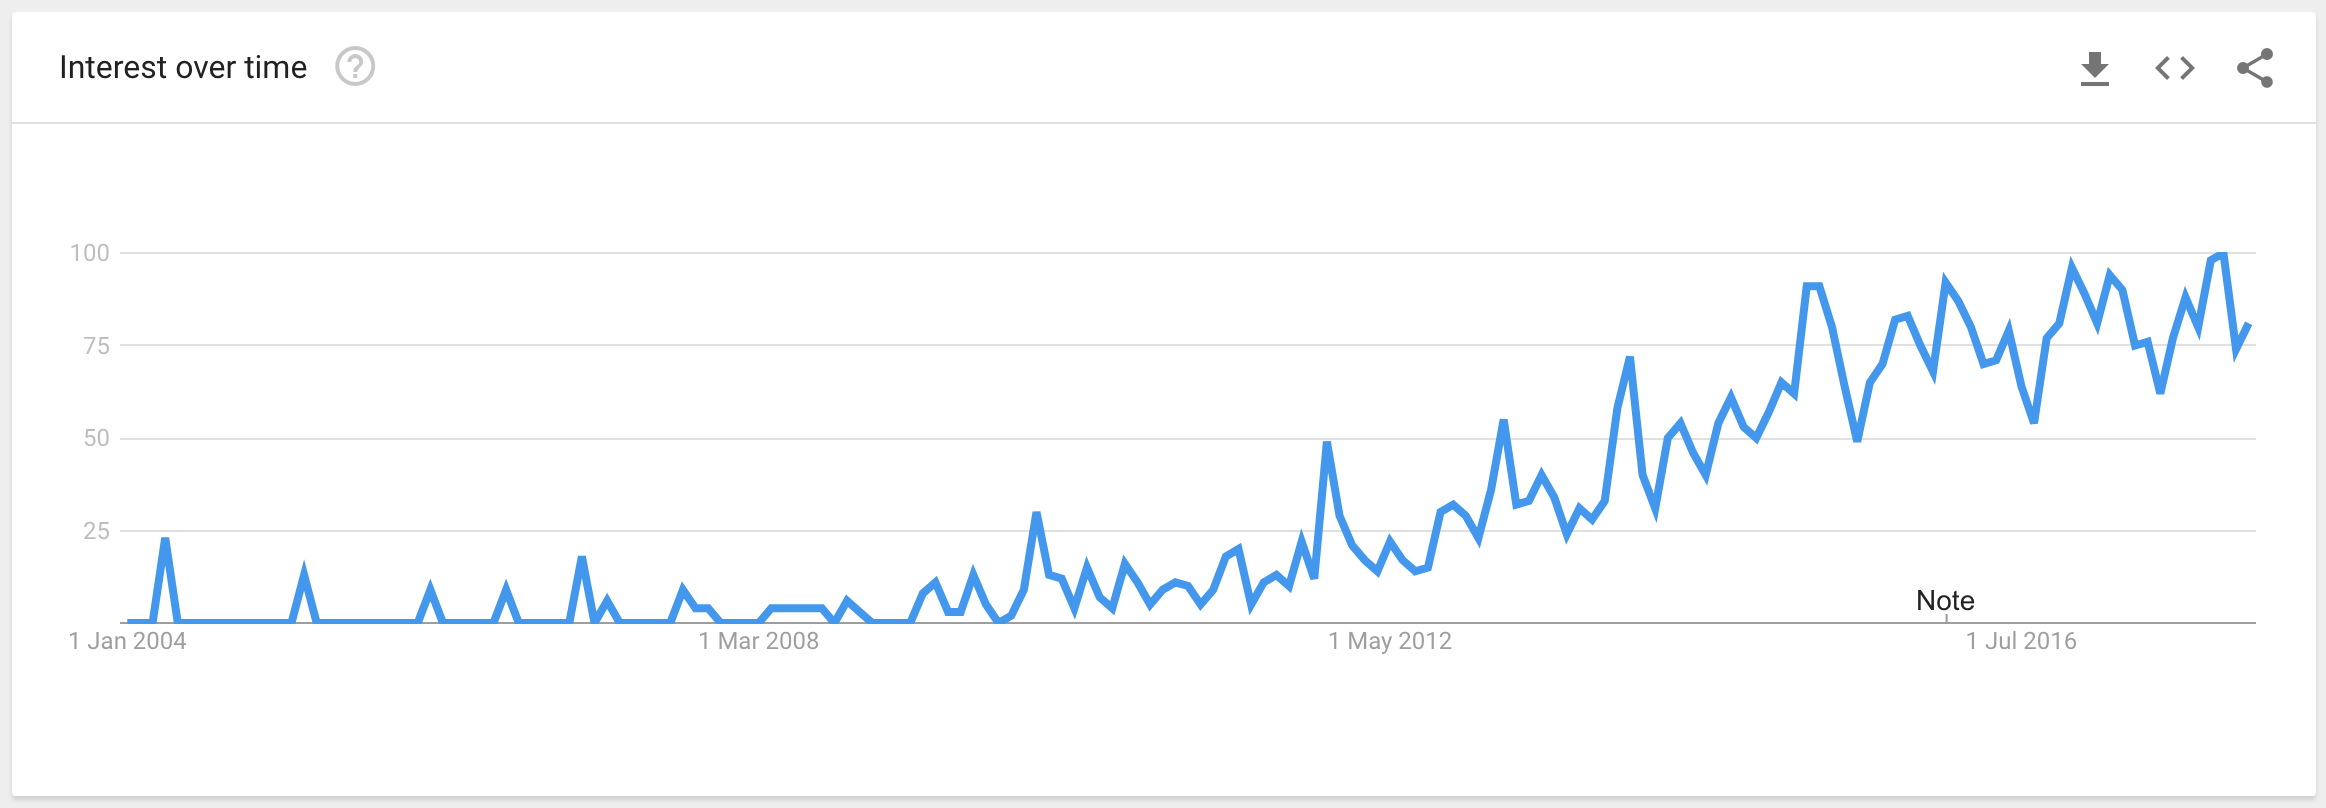
\includegraphics[width=\linewidth]{img/drone_interest_over_time_google.png}
  \caption{Google Trends for ``Drone Technology''. \cite{Google2018}}
  \label{fig:starship_citizen}
\end{figure}

Due to numerous advances in technology, drones are quickly advancing to the point where human input is no longer a necessity. This has led to many companies showing interest in integrating drones with their work in the coming years. \\

Although it may be an engineer's dream for a fully automated world, drones in particular are a harrowing reminder that there are real risks associated with them. There are already several incidents of drones crashing into planes and flying into areas they shouldn't, most notably near Heathrow airport\cite{BBCNews2017}.

\clearpage
All of this provides motivation to introduce some form of autonomous air traffic control system to navigate these drones to their respective destinations in a safe manner.\\

However, prior work has been done on the routing and navigation aspect of such a system\cite{Balaji2017}. In order for drones to truly take over more aspects of our lives, we must look at how they can provide a tangible benefit to specific use-cases. There is no doubt that simply removing the human element can save costs drastically, and there is none more exciting an application than with physical delivery networks.\\

The main factors that could prompt higher adoption of drones for delivery networks are cost, delivery speeds, and convenience. As figure \ref{fig:drone_del_cost} shows, drones can be both faster and cheaper than existing deliver options that consumers have access to.
\begin{figure}[!hbpt]
  \center
  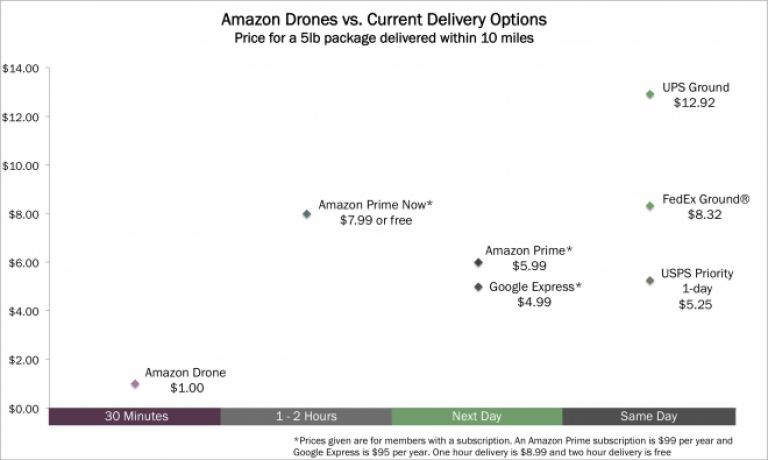
\includegraphics[width=\linewidth]{img/ark-invest-drones-analysis-768x460.png}
  \caption{How Amazon Air fits into the wider delivery market. \cite{Wang}}
  \label{fig:drone_del_cost}
\end{figure}

It appears then that Amazon stands to increase their margins considerably if they can successfully pull off their Prime Air initiative\cite{Welch2015}, but to do this they need to be able to handle the additional problems of scheduling and load balancing massive quantities of drones, on top of the existing routing problems. \\

In a more general sense, goods delivery networks have a lot to gain by optimising for profit, and to do this better we consider a variable delivery pricing mechanism that factors in the quality of service provided to the user. A high-priority product may warrant a higher delivery fee for quicker delivery but a similarly high penalty for being late.\\

At the same time, a low-priority product may not have any such penalty, instead opting for a low delivery fee. Being able to factor this new fee model when scheduling tasks and allocating drones may be the next step in the ongoing automation of last-mile delivery\cite{Joerss2016}.\\

Regardless of how such a model is implemented, it needs to be tested thoroughly before being deployed into production with actual drones. Considering a typical delivery drone could cost around \$100 to \$500\cite{Menon2013}, and that there is likely be a lot of failure before a working implementation, there could be several hundreds of thousand dollars worth of losses. \\

Therefore, our best port of call is to simulate scenarios that are as close to the real world as possible. One tech firm investigating how to produce richer, meaningful and more realistic simulations is \textit{Improbable}\cite{ImprobableWorldsLtd.2018a} - a London-based tech startup actively developing a distributed simulation platform called \textit{SpatialOS}\cite{ImprobableWorldsLtd.2018b}. \\

We aim to leverage the power of SpatialOS to produce novel simulations of a drone delivery network. The simulation will build upon existing routing solutions\cite{Balaji2017} and would aim to schedule deliveries based on a Quality of Service value curve. Furthermore, we wish to show how the profitability of a drone delivery network with this form of scheduling might compare to delivery networks that utilise a different scheduling mechanism.

%**********************************************%
\newpage
\chapter{Background}
We first provide an insight into new developments in the physical delivery network sector, and then specifically considerations to account for when integrating drone technology in our day to day lives. Additionally we summarise prior work completed by Imperial students on an autonomous air traffic control system for drones. \\

We then continue to discuss methods of prioritising a delivery network for financial gain. Finally, we give details about Improbable's SpatialOS and the reasoning for using this platform for the drone simulation.

\section{Future of Delivery Networks}
From the ancient days of Assyrian trade in 19 BCE \cite{stearns2001the}, to the modern day online market - the ability to trade goods and services has had a profound impact on the way we live our lives. Thanks to globalisation and the explosion of the internet, we are now able to use a service such as Amazon Prime and get goods delivered within days, if not hours, of purchasing through a simple click. Through it all, physical delivery networks enable this online retail behemoth. \\

As technology evolves, so too will these delivery networks - and many companies are currently looking into how to leverage upcoming tech\cite{Lee2016} in order to generate hype for their business and, more importantly, increase their profit margins. Some promising developments are delivery robots, autonomous cars and, of course, drones.

\subsection{Delivery Robots}
Delivery robots are unmanned devices that are designed to be operated on pavements and cycle lanes at low speeds of about 4 miles per hour\cite{Lee2016}. Although the unmanned device market is in its infancy, there are already prototypes hitting the market such as Starship's robot\cite{Laris2016}, which can hold upto 20-25 pounds, and Dispatch's ``Carry''\cite{Kokalitcheva2016}, that holds up to 100 pounds.

\begin{figure}[!hbpt]
  \center
  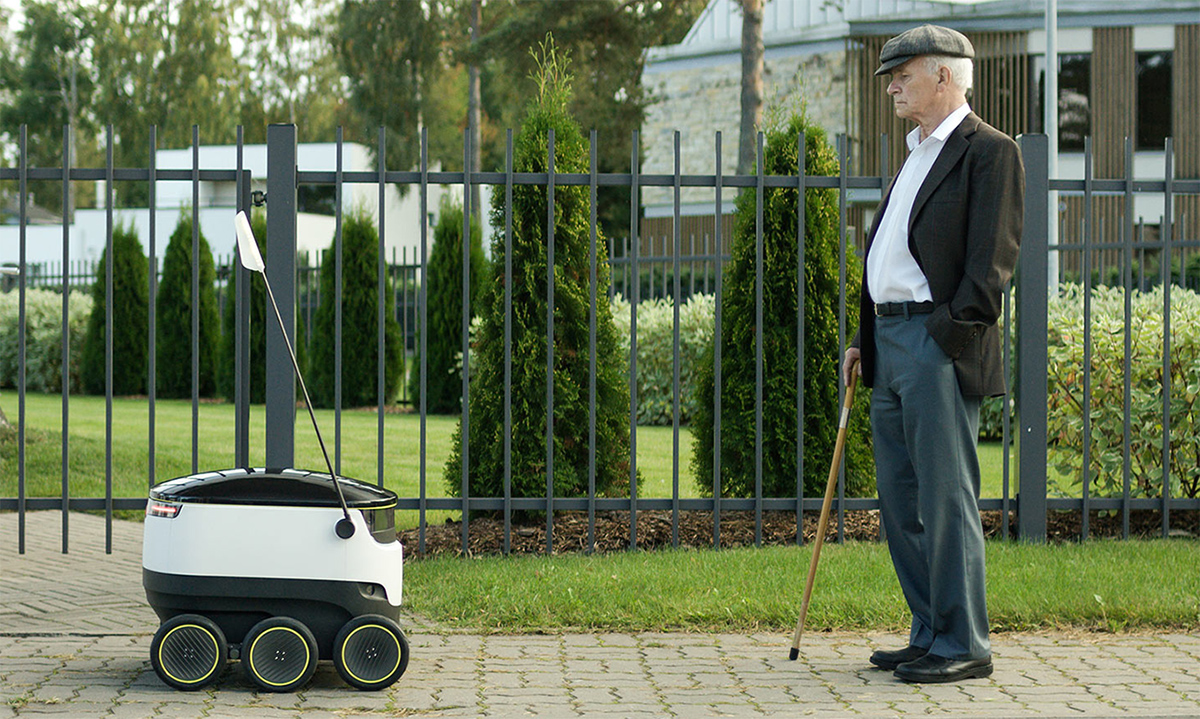
\includegraphics[width=\linewidth]{img/starship.jpg}
  \caption{Starship's robot confronting a senior citizen. Image from Engadget\cite{Souppouris2015}.}
  \label{fig:starship_citizen}
\end{figure}

Due to their on-the-ground nature, delivery robots are primarily designed for low-footfall suburban neighbourhoods, closed residential areas or campuses. They would be scheduled through an Uber-like application that may allow users to track the location of the robot, for the customer's knowledge, and to also unlock the robot once it reaches its destination\cite{Hohenadel2015}. \\

Thanks to their similarities to autonomous cars, they may have regulatory advantages compared to drones because much of the legislation coming through for autonomous vehicles can apply to delivery robots as well. However, there are profitability concerns because each robot can cost hundres of dollars and there is at this stage there is a high risk of failure, damage and even theft. \\

Despite some drawbacks, it is evident these robots are designed for short journeys in the so-called "first-mile delivery" sector - with exciting use cases being the delivery of flowers, groceries and possibly medication.

\subsection{Autonomous Vehicles}
Once the de-facto icon of science fictional futurism, autonomous cars are now a close reality. Companies such as Tesla are doing pioneering work in bringing self-driving cars\cite{Tesla2018} to the general consumer. Meanwhile, other businesses like Uber are experimenting with autonmous taxi services\cite{Gibbs2017}. \\

In fact, Google has obtained a patent for an autonomous delivery truck \cite{Hall-Geisler} with different compartments that could be unlocked by validated package recipients - much akin to an Amazon Locker-on-wheels. If not this, these vehicles could be used as an autonomous courier to pick-up locations that users could visit to retrieve their packages.

\begin{figure}[!hbpt]
  \center
  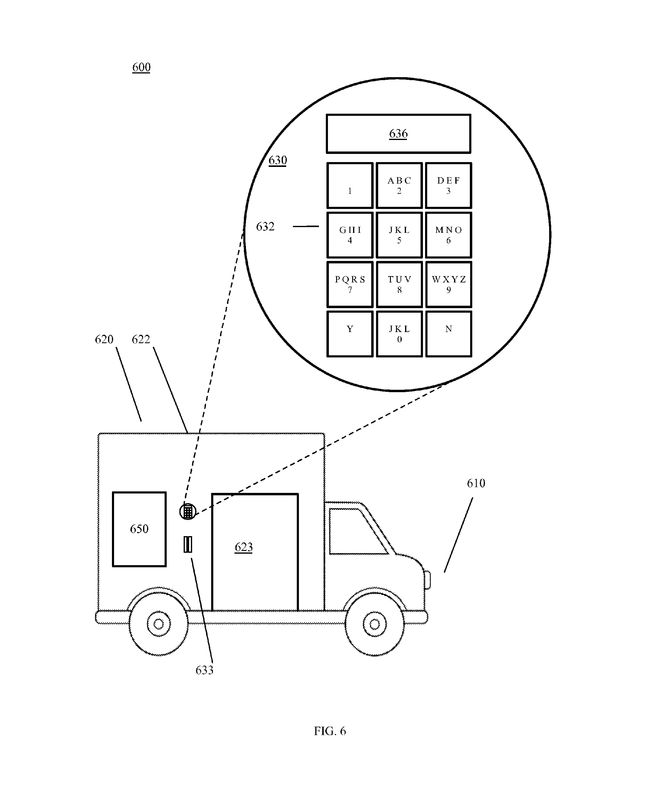
\includegraphics[width=0.4\linewidth]{img/google_truck_patent.jpeg}
  \caption{Illustration of Google's Delivery Truck. \cite{google_truck_patent}}
  \label{fig:google_truck_patent}
\end{figure}

Although current regulations dictate that a driver must remain present in the vehicle in the event of software performing differently to expections, this is a necessary precaution whilst driverless systems are still being tested - with further amendments to these laws in sight once these systems can be deemed safe for public use. \cite{Bowcott2017}

\newpage
\subsection{Drones}
The concept of drones has been around for decades, particularly in the military, but only in recent times has the technology evolved to a point where anyone can walk into a consumer electronics store and purchase a drone for their own private use. Though these are manned, it is admirable that many witness the benefits of drones in film/television\cite{Verrier2015}, agriculture\cite{Jarman2016}, policing\cite{BBCNews2017a} and other exotic activities\cite{Roberts2016}. \\

Being able to fly allows drones to not be held hostage to traffic jams or congestion - after all, the sky is a far greater expanse than even the most intricate of road networks. Not only that, they can literally travel ``as the crow flies'' - allowing them to access remote and previously hard-to-reach areas.\\

Despite several near-misses \cite{Davies2017} and accidents\cite{BBCNews2016} at just Heathrow airpot alone, engineering teams across the world are working on ways to improve drone visibility to its surroundings - one such technology being automatic dependent surveillance-broadcast (ADS-B) \cite{Dillow2015}. Drones with ADS-B work by determining their own geolocation and velocity in order to broadcast this back to the global network.\\

ADS-B is already widely used in aircraft, enabling flight-tracking services such as flightradar24 to exist\cite{Flightradar242018}, but recent developments have allowed the ADS-B units to be compact and cost-effective enough to be suitable for drones. As more drones adopt this technology, instead of having to get instant updates from a drone directly, autonomous drone traffic control systems could make use of the shared global network for their scheduling and routing calculations. \\

Over time, an increasing percentage of the world's drones will likely join these shared autonomous systems. This could enable different delivery networks to manage their own fleets as their own air traffic controllers, all the while making use of the shared pool of readable data to identify, intercept and avoid drone collisions at the earliest stage in their pathfinding as possible.

\section{Amazon Prime}
Amazon Prime is a paid subscription service that Amazon offers to users, giving unlimited access to their video and music streaming services as well as providing free same-day and next-day delivery on a large majority of goods sold on their platform. The Prime service applies to products that are either sold directly by Amazon or fulfilled on behalf of a third-party merchant.

\subsection{Fulfilment by Amazon}
One of the services Amazon provides to merchants is the \textit{Fulfilment by Amazon} service, where goods are held at Amazon depots until a user purchases a product. The fee paid by the merchant for Amazon to take care of delivery depends on the duration of time the product is held by Amazon as well as the type of package and weight of the product.

\begin{figure}[!hbpt]
  \center
  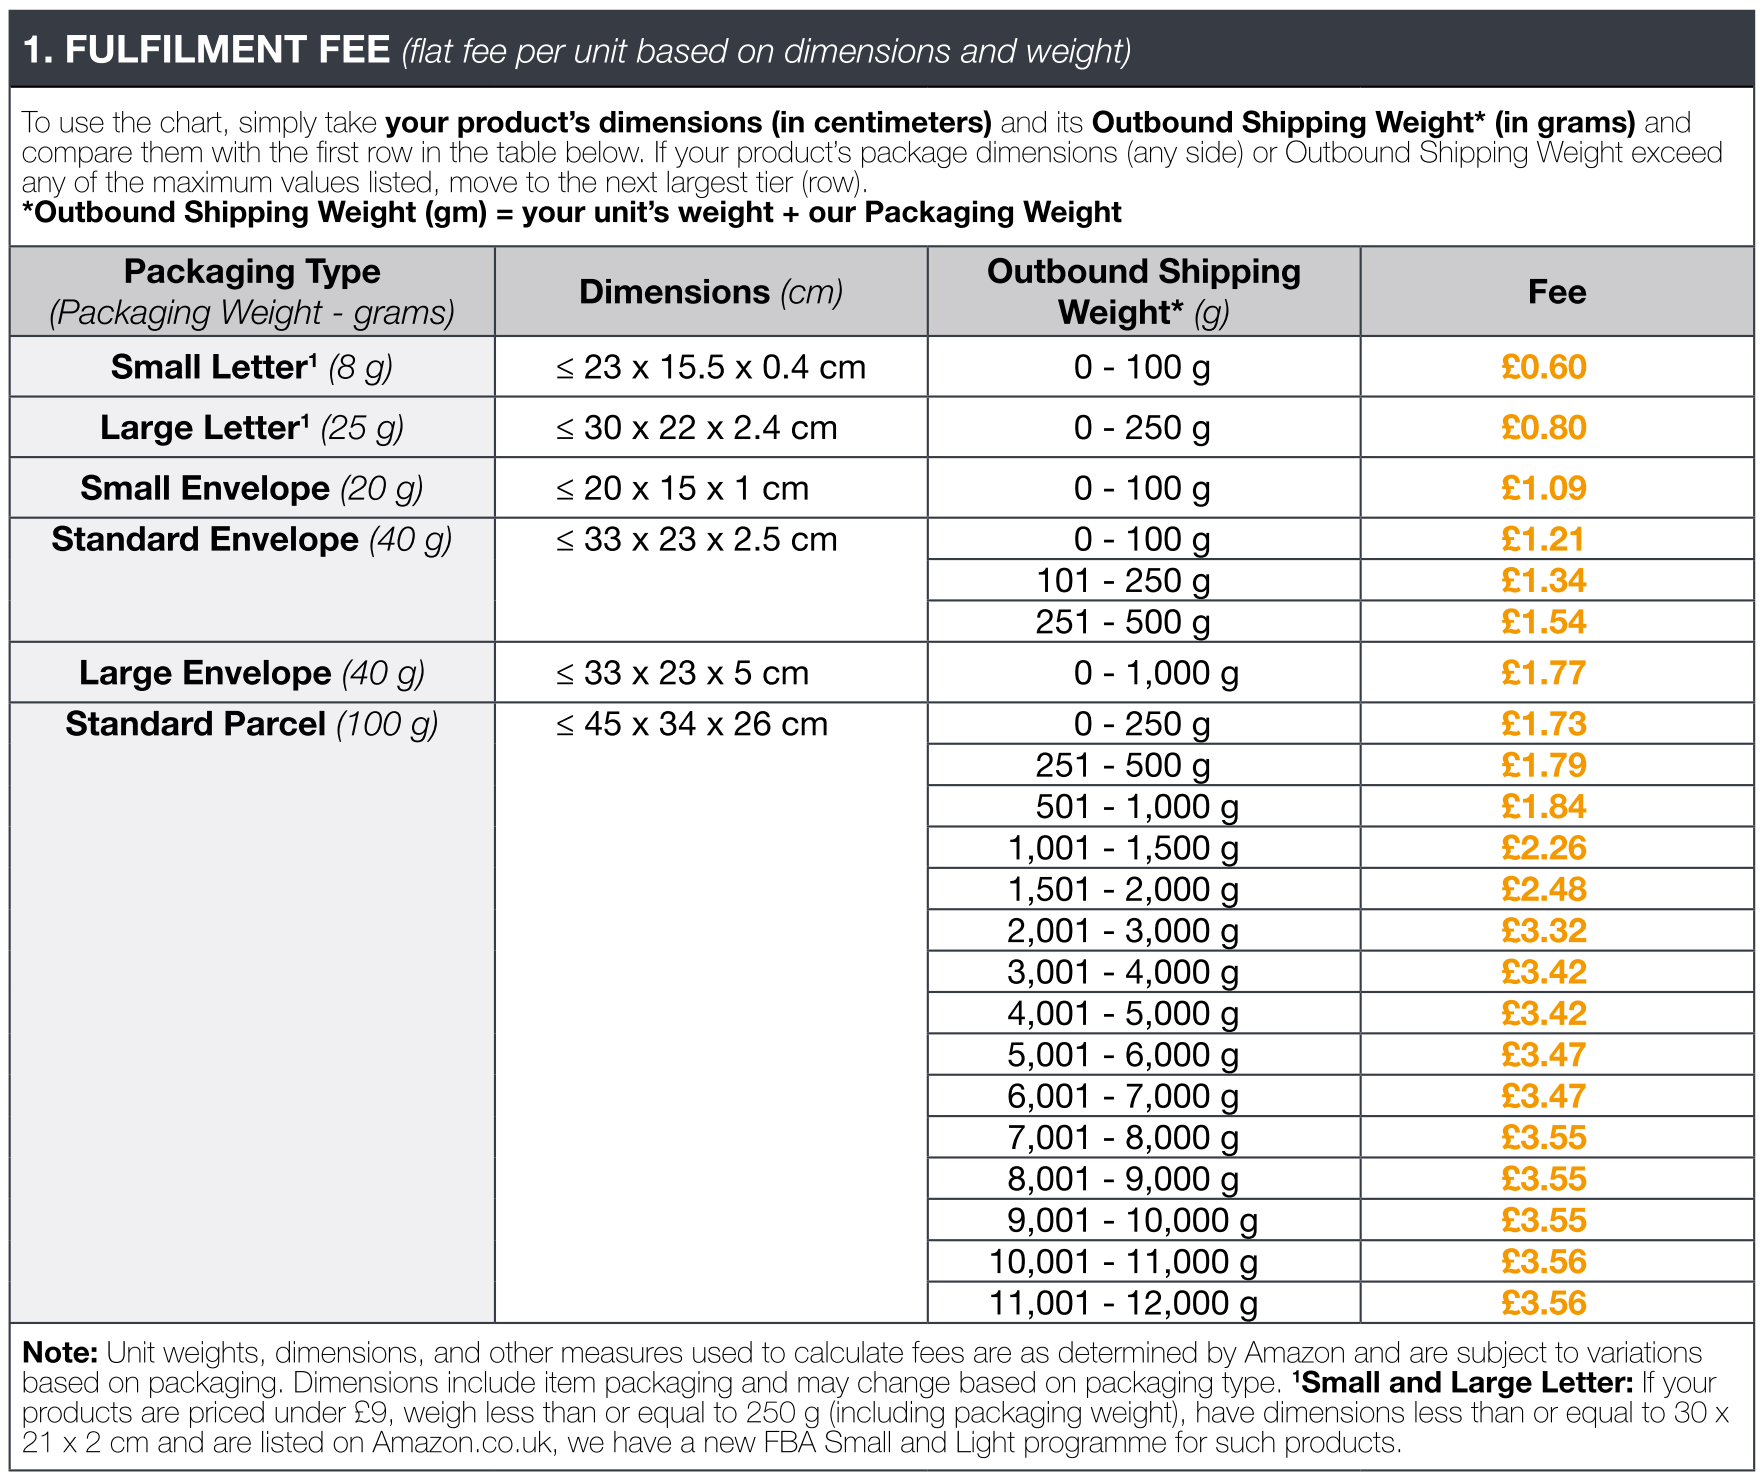
\includegraphics[width=0.9\linewidth]{img/fulfilled_by_amazon_table.png}
  \caption{Fulfilment fees for standard-size items on Amazon UK. \cite{Channel2017}}
  \label{fig:fulfilled_by_amazon_table}
\end{figure}

\newpage
An incentive for merchants to join this scheme is to attract customers with the same-day and next-day delivery that Amazon Prime offers. This allows them to piggy-back off the existing delivery network that Amazon has developed for significantly lower fees (Figure \ref{fig:fulfilled_by_amazon_table}) than if they were to store the package and source a distributor for themselves.

\subsection{Amazon Prime Air}
In December of 2013, Amazon announced their intentions to research and develop their own drone delivery service dubbed \textit{Amazon Prime Air} \cite{Amazon.comInc.2013}. Amazon intends this service to deliver packages within 30 minutes of an order being placed, with a maximum package weight of 5 pounds (approximately 2.27 kg).\\

Following this, in November of 2015 the company enlisted the help of Jeremy Clarkson to give a closer look at a more developed drone prototype \cite{Amazon.comInc.2015b}, describing how Prime Air would fit into the lives of modern families. Just over a year later, Amazon released a video demonstrating a fully autonomous delivery using Prime Air \cite{Amazon.comInc.2016}.

\begin{figure}[!hbpt]
  \centering
  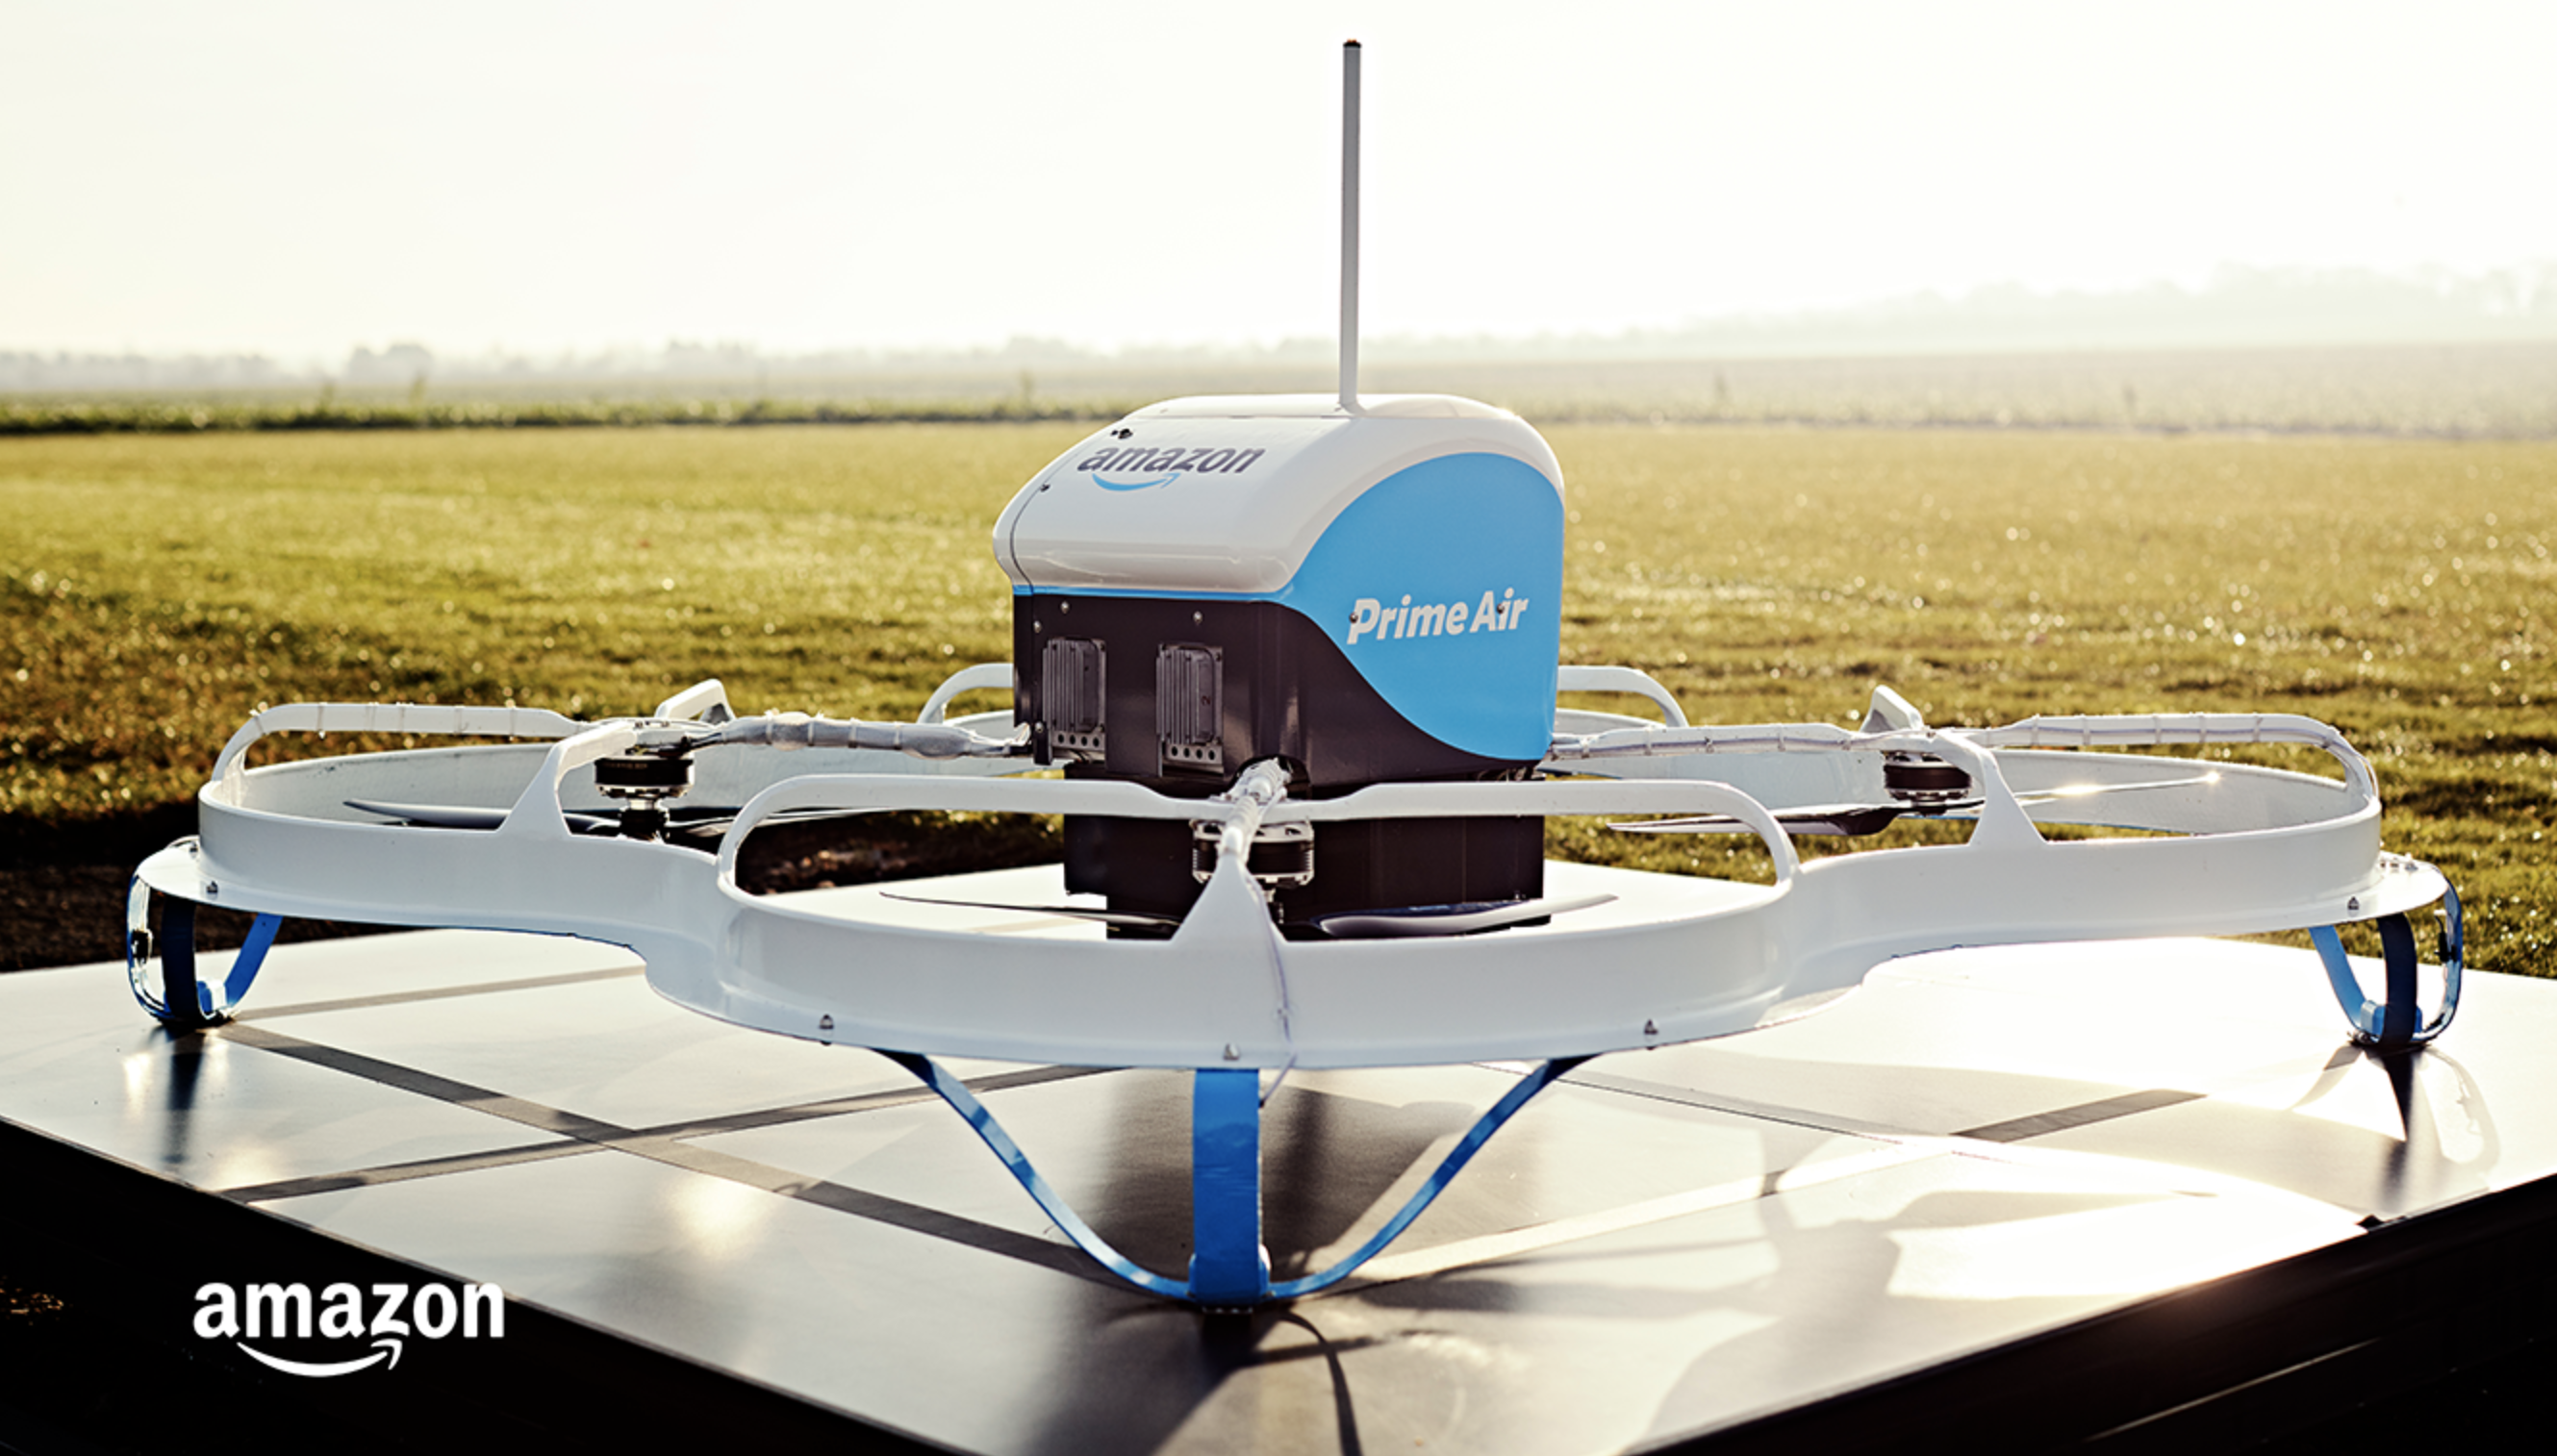
\includegraphics[width=0.6\textwidth]{img/amazon_prime_air_drone.png}
  \caption{One of Amazon's Prime Air prototypes. \cite{Amazon.comInc.}}
  \label{fig:prime_air_example}
\end{figure}

One of the many roadblocks to scale this technology out across the country is regulatory approval. Since drones are a new technology that improve in leaps and bounds each year, authorities and enterprises are careful to make hasty judgements that either hamper drone adoption or cause civilian harm. To this end, Amazon are also suggesting proposals to how airspace can be best utilised by drones. \cite{Amazon.comInc.2015} \cite{Amazon.comInc.2015a}

\section{Drone Considerations}
Drones stand to be a revolutionary part of our lives as we welcome the new, incoming era of automation. However, to be practical there are a few key concepts one must understand to ensure that they remain a help and not a hinderence to mankind.

\subsection{No Fly Zones}
No Fly Zones (which we will abbreviate as NFZs) are geographical areas where a drone is not allowed to enter or fly at any altitude. Examples of these may include Hyde Park, Buckingham Palace, airports and military locations. Typically these are static obstacles that will always remain a NFZ, however we could also consider cases when they could be created dynamically.\\

Suppose there was an issue of national security, it would be beneficial for the security and intelligence services to set up a temporary NFZ around areas where they deem a risk so that they can conduct their own operations without worry of external parties interfering with the situation.

\subsection{Other Drones}
Naturally we would want to make sure that we avoid colliding into other drones as well. In a perfect system, a single air traffic controller would have totalitarian dominance over all drones that take to the skies - however this is not \textit{Black Mirror} and we have to assume that there will always be drones that this system will not be able to control or predict. \\

Nonetheless, a system can ensure that it navigates drones under its control as best as it can, avoiding these external drones and other rogue drones that may be flying with the sole intention of causing problems to others.

\clearpage
\subsection{Manned Aviation}
Manned Aviation is any form of airborne transport with humans on board. This would include passenger jets, private jets, helicopters and other miscallaneous vechicles. For simulation purposes, we can consider these to have straight paths from a start to an end because relative to the zig-zagging of drones - they are effectively straight.\\

It is paramount to avoid collisions with manned aviation because there is a high risk of human calamity, in addition to the bad press and financial costs associated with such an air traffic incident.

\subsection{Toll Zones}
Toll Zones are geographical areas where a drone has to pay an extra fee to pass through at any altitude. It is a very similar idea to the one that led to Congestion Charges being applied to much of central London. By restricting certain areas only to those who are willing to pay the fee to use the airspace, it reduces the density of air traffic in a specific area.\\

These charges could also be used as an incentive to reduce pollution in the toll zone, and the additional revenue generated by the toll fees could be used towards the drone-related systems in place within the zone.

\section{Autonomous Air Traffic Control (AATC)}
\subsection{What is AATC?}
During the Autumn Term of the 2016-17 academic year, several students undertook a group project in association with Microsoft and Altitude Angel to produce an autonomous air traffic control system. The goal of the project was to safely navigate drones from their start to their end goals, whilst avoiding obstacles and taking the shortest possible path to minimise battery use.

\clearpage
\subsection{Technical Overview}
AATC has a simple client-server architecture, where drones connect to the REST service to send their telemetry information and goal waypoints every second. The server sends back direction recommendations to navigate the drone to its destination. \\

Because it would have been too expensive to trial the system on actual drones, a test bench was also implemented that would simulate the drones polling the server and responding to its recommendations. This test bench produced a set of simulation data, that is then available to view on the AATC visualiser. \cite{Balaji2017a}

\begin{figure}[!hbpt]
  \center
  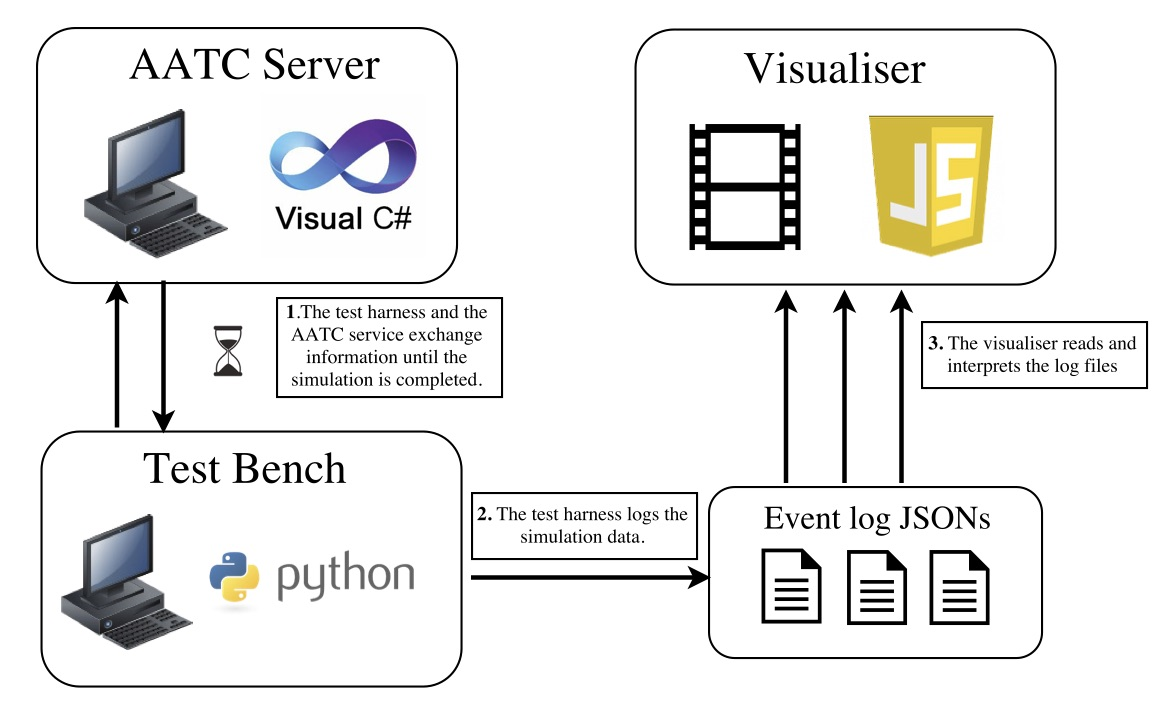
\includegraphics[width=\linewidth]{img/aatc_tech_overview.jpg}
  \caption{Technical Overview of AATC. \cite{Balaji2017}}
  \label{fig:aatc_tech_overview}
\end{figure}

The system was designed with three challenges in mind. The first challenge was to route drones from their origins to their destinations, and secondly, to ensure they avoided collisions with both static and dynamic obstacles - such as the ones mentioned in Section 2.3. The last challenge is to design the system in such a way that it would be able to scale to hundreds and thousands of drones.

\clearpage
To this end, a \textit{Global Layer} was built to deal with static obstacles (such as NFZs) by calculating a path for the drone around NFZs before it begins its journey. The second problem was tackled with a \textit{Reactive Layer} that handles non-static obstacles (such as manned aviation and other drones). This is the layer that would be providing the real-time updates to drones as they poll the server every second. \\

\begin{figure}[!hbpt]
  \center
  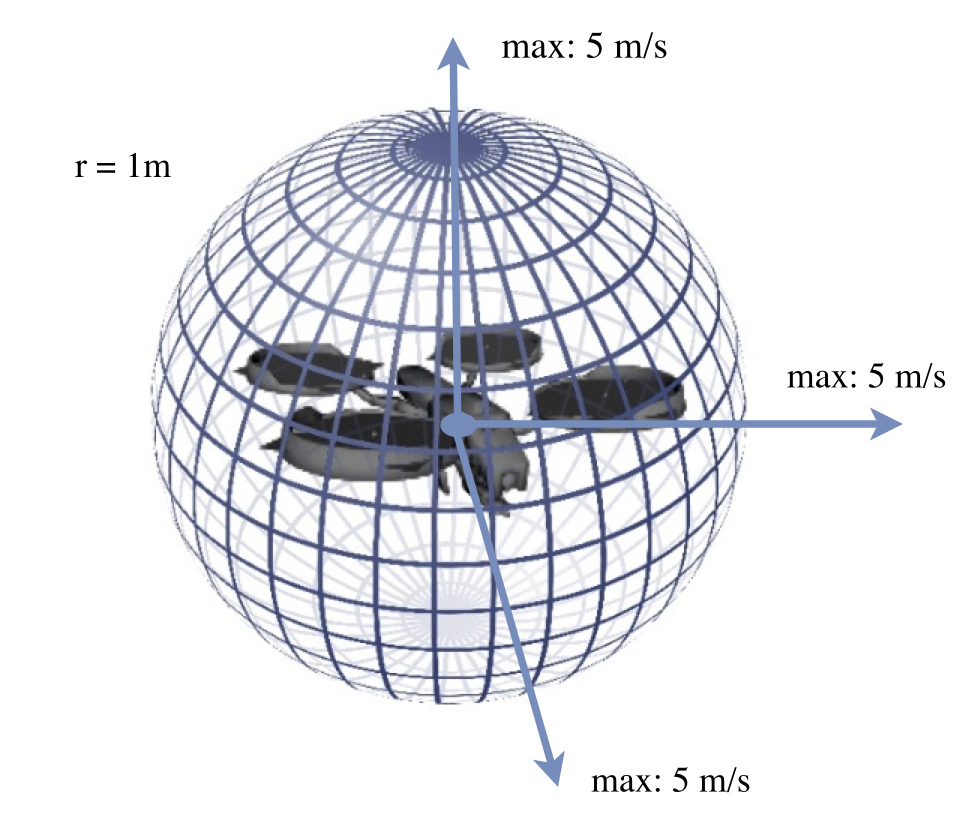
\includegraphics[width=0.8\linewidth]{img/edrone.jpg}
  \caption{The default AATC drone model. \cite{Balaji2017}}
  \label{fig:edrone}
\end{figure}

Only one drone type was used in AATC, with its specification outlined in Figure \ref{fig:edrone}. It has a radius of 1m and a maximum velocity in any direction of 5 metres per second.

\section{The Global Layer}
The Global Layer holds the static representation of the world so that given a start and end, it can compute an optimal set of waypoints that a drone should follow - thereby dealing with AATC's path-finding problem.

\subsection{Dijkstra's Algorithm}
Dijkstra's algorithm is a popular algorithm to find the shortest paths between nodes in a graph. When using a co-ordinate grid system, each coordinate could represent a node in a graph and thus the algorithm can also be used to find the shortest path between a source and destination. \\

However, in the real world, we also have to consider the cost of computation and potentially make use of heuristics in order to return the shortest path given a limited amount of time. Especially in the drone case, we want to compute a good path as quick as possible in order to let the drone proceed along its way.

\subsection{A* Algorithm}
Enter, the A* algorithm. This algorithm is a generalisation of Dijkstra's algorithm that reduces the number of nodes explored during the search process by use of a heuristic - typically a minimum distance to the destination. A benefit over Dijkstra in particular is that it considers the distance already traveled into account, which aids the heuristic mechanism. \\

Naturally, by searching less nodes on a graph, less computation is performed and therefore A* has better performance than just using a pure form of Dijkstra's algorithm.

\begin{figure}[!hbpt]
  \center
  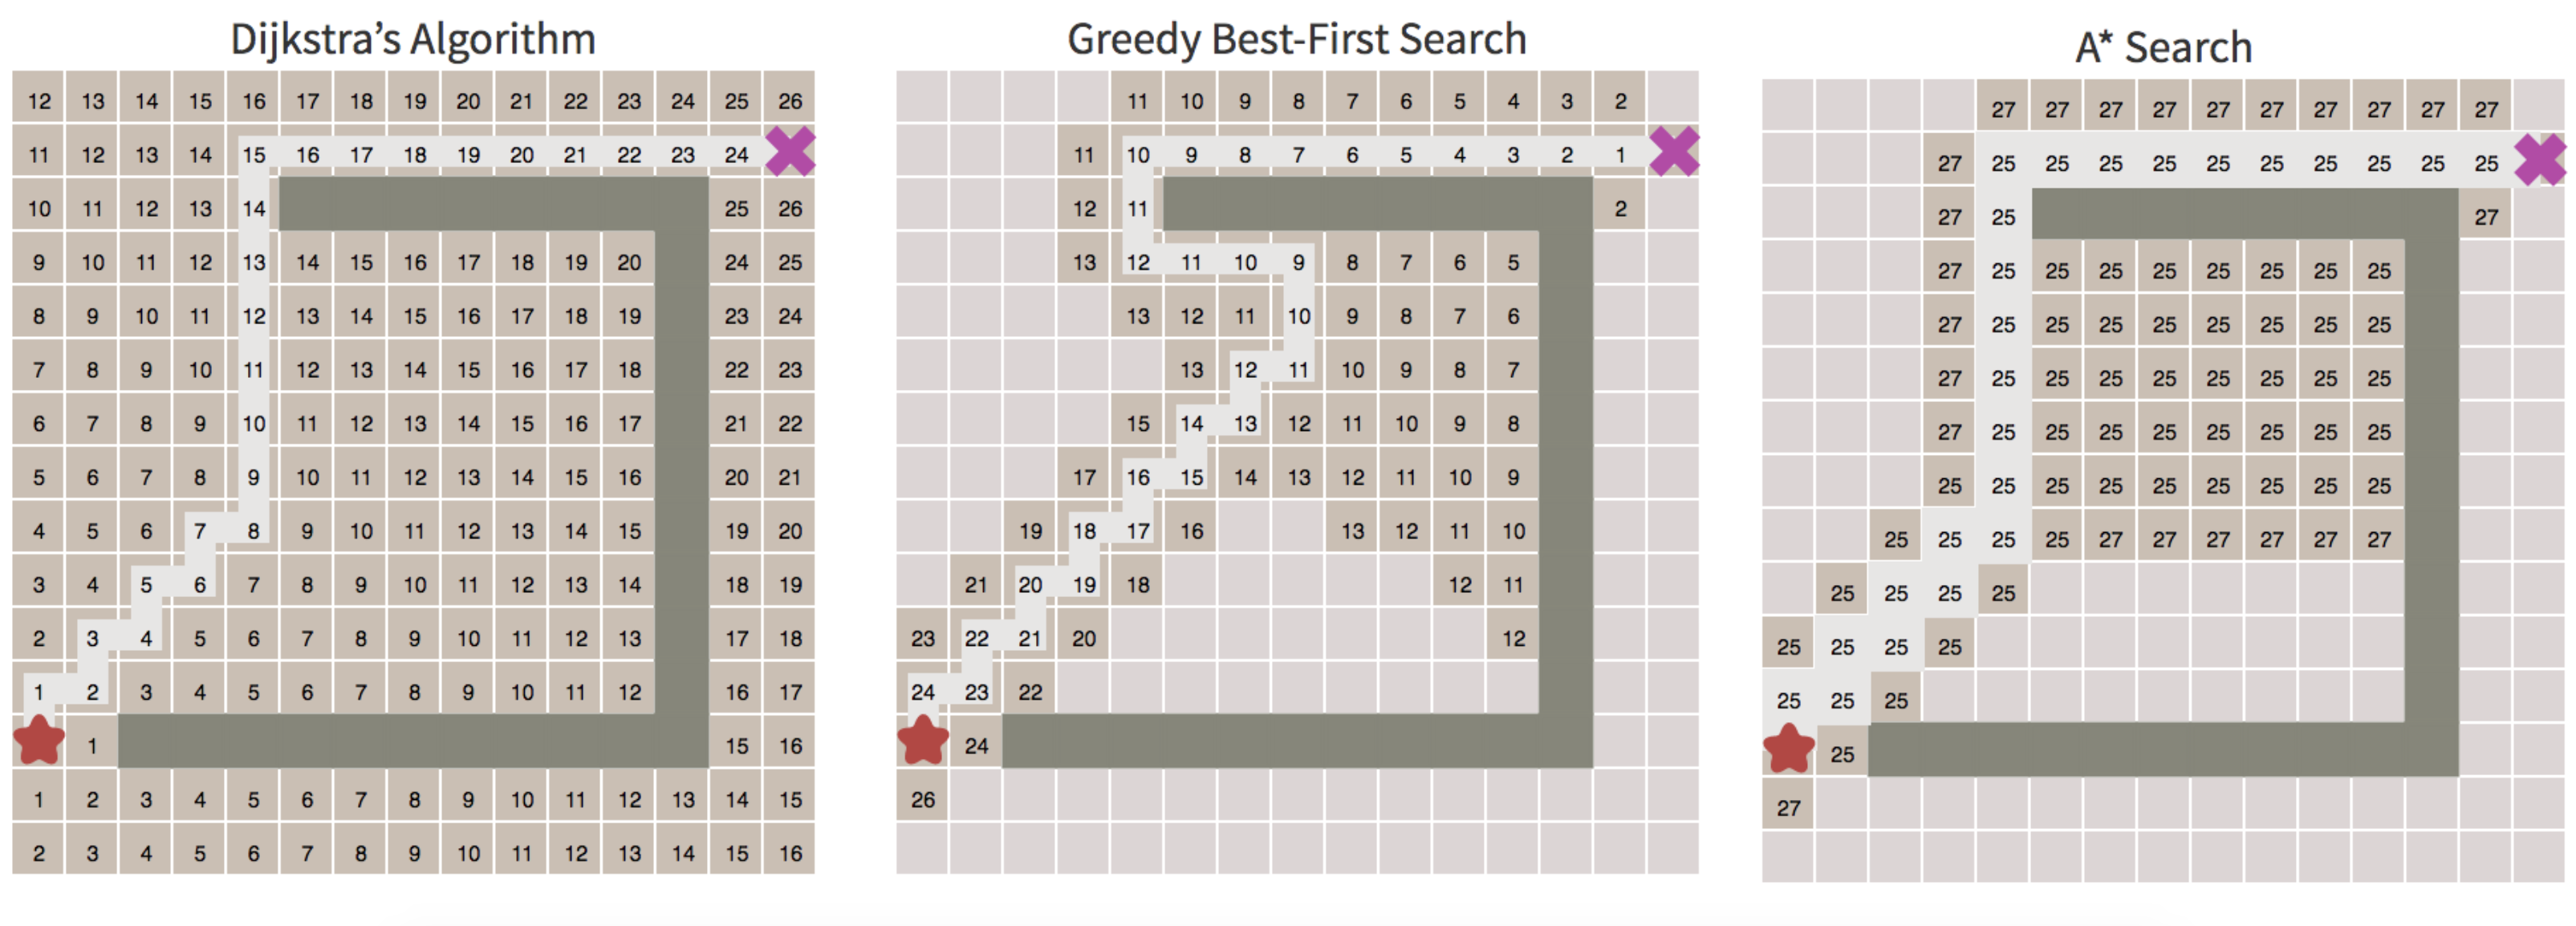
\includegraphics[width=\linewidth]{img/search_comparison.png}
  \caption{Comparing popular search algorithms. \cite{Balaji2017}}
  \label{fig:search_comparison}
\end{figure}

\clearpage
But for all these positive aspects, one must remember that our use for this algorithm is to compute paths in a real world, which is not necessarily split up into a nice, clean grid. So we turn our attention to a modification of the A* algorithm: Theta*.

\subsection{Theta* Algorithm}
The Theta* algorithm is an any-angle pathfinding algorithm based on the A* algorithm that introduces Line of Sight (LOS) checks, which means that each jump from node to node in the returned path can be at any angle and not just up, down, left or right. This neat addition allows Theta* to be capable of finding near-optimal paths with a runtime comparable to A* \cite{Uras2015}.\\

Being able to get as short a path as possible is absolutely vital in the drone use-case because they have limited flying time. After all, their batteries can only last so long before they need to be recharged. Therefore, it is important to ensure drones travel as little distance as possible in order to maximise the number of times they can be used between charges.

\begin{figure}[!hbpt]
  \center
  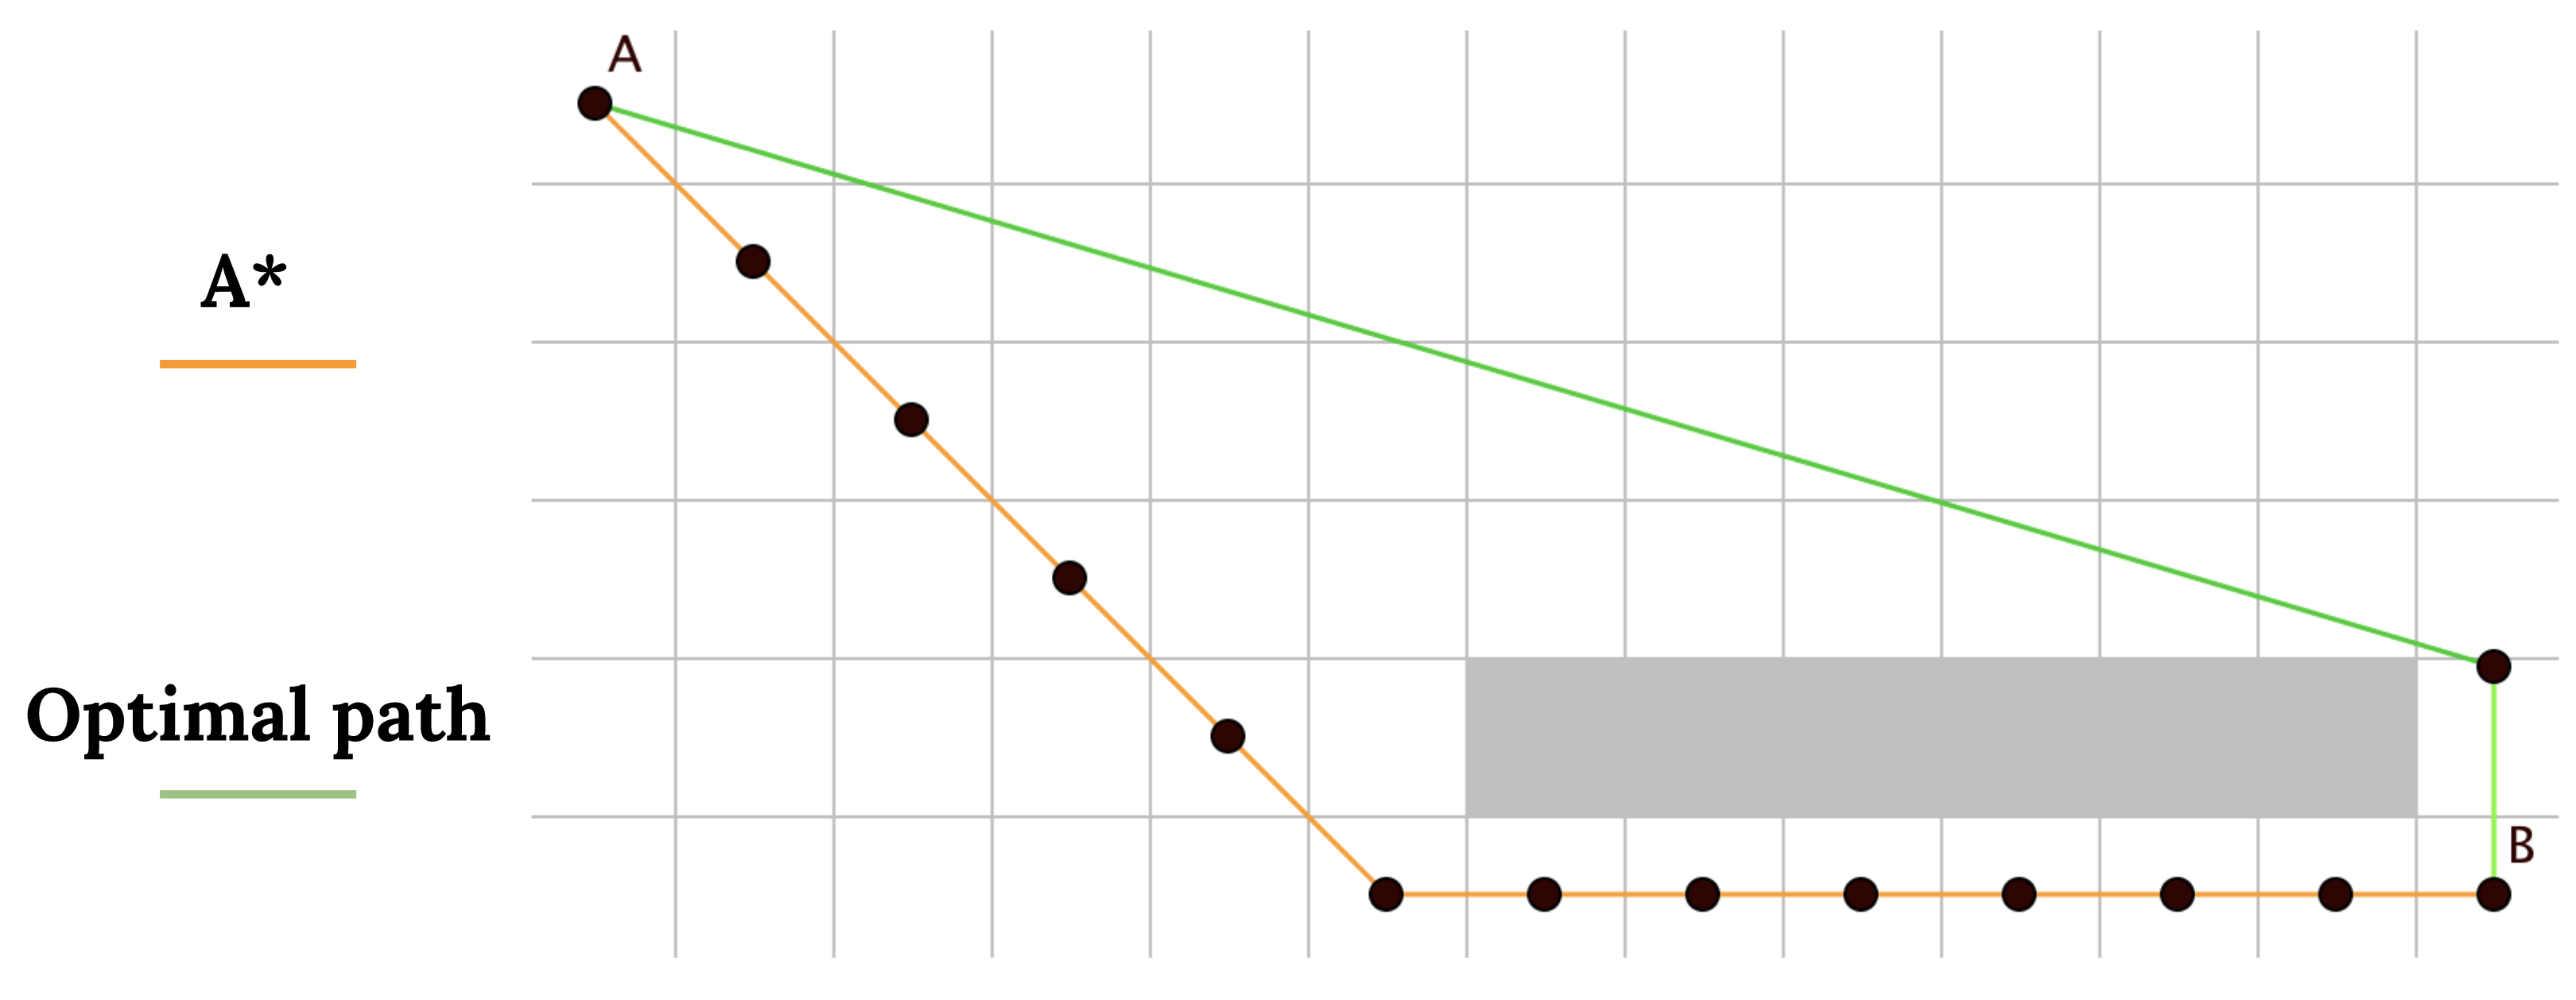
\includegraphics[width=\linewidth]{img/a_star_vs_optimal.png}
  \caption{A* vs Optimal Path. \cite{Balaji2017}}
  \label{fig:a_star_vs_optimal}
\end{figure}

\clearpage
\subsection{Lazy Theta* Algorithm}
A further optimisation is to reduce the number of LOS checks performed, as found in another paper by the original authors of the Theta* algorithm\cite{Nash2010}. This algorithm assumes every node is in line of sight of its parent, and the LOS check is only performed once the child node is expanded on. If this turns out to be false, then the algorithm defaults to a typical A* approach. Reducing the number of LOS checks therefore improves the algorithm's overall performance.

\subsection{Conclusions}
As seen on Table \ref{tab:aatc_exec_time}, A* has far better execution times than both Theta* variants but when we get to Table \ref{tab:aatc_total_drone_distance} it is evident that Lazy/Theta* produces better paths because the total distance travelled by drones is fewer. Therefore, Lazy Theta* was chosen as the core algorithm for the Global Layer.

\begin{table}[!hbpt]
\centering
\begin{tabular}{|l|c|c|}
\hline
\multicolumn{1}{|c|}{Test Case} & A* & \multicolumn{1}{l|}{Theta* and Lazy Theta Star} \\ \hline
Queen Threat & 6.11 & 5.98 \\ \hline
The Imperial Tunnel & 10.83 & 10.22 \\ \hline
The Great London Beehive & 52.63 & 49.77 \\ \hline
The Nightmare of Hyde Park & 118.4 & 115.32 \\ \hline
The Great Wall of Imperial College & 16.37 & 15.46 \\ \hline
Multi Drone collision & 15.27 & 14.82 \\ \hline
\end{tabular}
\caption{Total path distances for all drones (in km). \cite{Balaji2017}}
\label{tab:aatc_total_drone_distance}
\end{table}

\begin{table}[!hbpt]
\centering
\begin{tabular}{|c|c|c|c|}
\hline
Test Case                          & A*                                                          & \multicolumn{1}{l|}{Theta*}                                   & \multicolumn{1}{l|}{Lazy Theta*}                              \\ \hline
Imperial Tunnel                    & \begin{tabular}[c]{@{}c@{}}118\\ 120\\ 121\end{tabular}     & \begin{tabular}[c]{@{}c@{}}141\\ 138\\ 137\end{tabular}       & \begin{tabular}[c]{@{}c@{}}124\\ 132\\ 129\end{tabular}       \\ \hline
Imperial Tunnel Mean               & 119.7                                                       & 138.7                                                         & 128.3                                                         \\ \hline
The Great London Beehive (GLB)           & \begin{tabular}[c]{@{}c@{}}859\\ 916\\ 894\end{tabular}     & \begin{tabular}[c]{@{}c@{}}1318\\ 1486\\ 1555\end{tabular}    & \begin{tabular}[c]{@{}c@{}}1166\\ 1075\\ 1201\end{tabular}    \\ \hline
The GLB Mean                       & 889.7                                                       & 1453                                                          & 1147.4                                                        \\ \hline
The Nightmare of Hyde Park (NHP)        & \begin{tabular}[c]{@{}c@{}}9771\\ 9687\\ 10118\end{tabular} & \begin{tabular}[c]{@{}c@{}}28436\\ 27970\\ 28273\end{tabular} & \begin{tabular}[c]{@{}c@{}}21330\\ 24786\\ 21609\end{tabular} \\ \hline
The NHP Mean                       & \multicolumn{1}{l|}{9858.7}                                 & \multicolumn{1}{l|}{28226.4}                                  & 22575                                                         \\ \hline
The Great Wall Of Imperial College (GWIC) & \begin{tabular}[c]{@{}c@{}}394\\ 447\\ 416\end{tabular}     & \begin{tabular}[c]{@{}c@{}}913\\ 910\\ 912\end{tabular}       & \begin{tabular}[c]{@{}c@{}}838\\ 840\\ 841\end{tabular}       \\ \hline
The GWIC Mean                      & 419                                                         & 911.7                                                         & 839.7                                                         \\ \hline
\end{tabular}
\caption{Execution times for pathfinding algorithms on AATC test cases. \cite{Balaji2017}}
\label{tab:aatc_exec_time}
\end{table}

\newpage
\section{The Reactive Layer}
Given the list of waypoints that the Global Layer generates, the Reactive Layer's task is to provide the right speed and direction to drones whilst taking into consideration any dynamic obstacles that the drone may face, such as manned aviation, other drones and potentially dynamic NFZs.

\subsection{Artificial Potential Fields (APF)}
A novel way to approach this layer is to create an Artificial Potential Field (APF) in the area the drone operates in, and give each point in this field a potential\cite{Zhu2016}. By having a low potential for the destination and large potentials at obstacles, the drone simply has to move in a way to get to point of lowest potential. It is analogous to a magnet in a magnetic field, repelled by obstacles and attracted to its destination. \\

Although one might argue that the Global Layer is not needed anymore because the Reactive Layer solves the pathfinding problem, there are a few issues that arise with this idea. As Figure \ref{fig:apf_comp} shows, a U-shaped object poses a problem because the drone may be attracted to the destination and then quickly repelled by the obstacle, and then back to being attracted - and this cycle is seemingly endless.

\begin{figure}[!hbpt]
  \center
  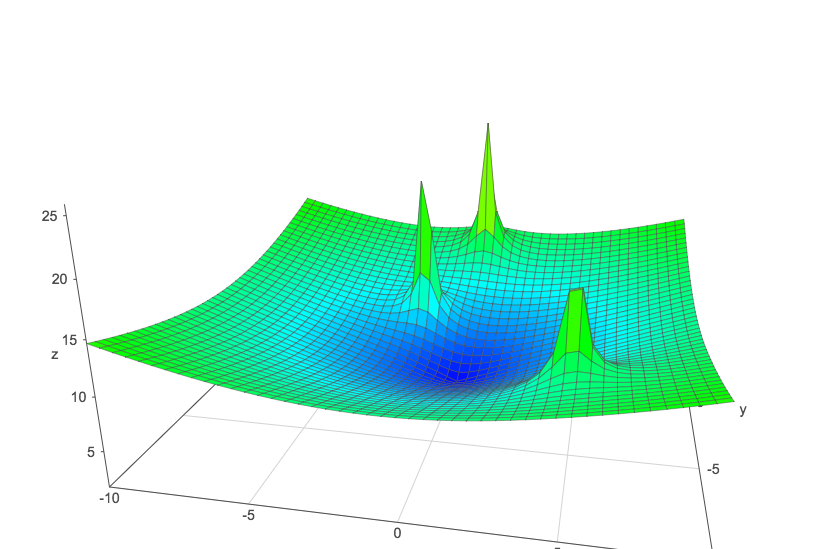
\includegraphics[width=0.9\linewidth]{img/obst.png}
  \caption{APF with obstacles (green peaks) and a destination (blue trough). \cite{Balaji2017}}
  \label{fig:obst}
\end{figure}

\newpage
By introducing a random element, as in Rotating APF, the object is repelled in a slightly different direction each time to make it out of the trap and eventually reach its destination. Even this method, however, does not actually guarantee that the drone makes it past the U-shaped obstacle because it depends on how the random element behaves and also whether the drone has enough battery to be loitering for long.

\begin{figure}[!hbpt]
  \center
  \includegraphics[width=\linewidth]{img/apf_comp.png}
  \caption{Pure APF vs Rotating APF vs AATC Implementation. \cite{Balaji2017}}
  \label{fig:apf_comp}
\end{figure}

Clearly, integrating both layers proves most fruitful - as the waypoints generated by the Global Layer are used to quite literally navigate around the problematic aspects of the Reactive Layer. This integration that was implemented in the AATC project.

\subsection{Equations for APF}
The full set of equations used to obtain the recommended unnormalized velocity $v_{raw}$ of the drone is:
$$U_a = \rho_ad_{goal}$$
$$U_r =  \begin{cases}
      \rho_r\frac{1}{d_{obst} - d_{safe}} & d_{obst} \leq d_{influence}   \\
      0 & otherwise \\

   \end{cases}
$$
$$U_{ret} = \rho_{ret}d_{last}$$
$$U = U_a + U_r + U_{ret}$$
$$\bm{v_{raw}} = \nabla U$$

where $\nabla U$ is the gradient of U, and U is the magnitude of potential at a point\cite{Balaji2017}. Since $\nabla U$ is the recommended velocity, it can be computed from first principles:
$$\nabla U(x,y,z) = \colvec{3}
                {\frac{\delta U(x,y,z)}{\delta x}}
                {\frac{\delta U(x,y,z)}{\delta y}}
                {\frac{\delta U(x,y,z)}{\delta z}}
                  \approx \colvec{3}
                {U(x + 1,y,z) -  U(x,y,z)}
                {U(x,y + 1,z) -  U(x,y,z)}
                {U(x,y,z + 1) -  U(x,y,z)}$$

The recommended velocity can now be computed by first calculating the potential at 4 points. To calculate the potential at a given point, one must find the sum of:
\begin{itemize}
  \item $U_a$ - attraction potential using euclidean distance to next waypoint.
  \item $U_r$ - repulsion potential using euclidean distance to nearest obstacle.
  \item $U_{ret}$ - return potential using euclidean distance to point from last time step.
\end{itemize}

To allow drones to gently come to their goals instead of shooting past and potentially missing, the recommended speed is calculated by taking the minimum of the drone's max speed and the distance to the goal:
$$ speed = min(max\_speed, d_{goal}) $$

The gradient $\nabla U$ is then normalised to be a unit vector before being multiplied by the speed to compute the final velocity.

\subsection{Genetic Algorithm}
By paying close attention to Section 2.6.2, we can identify several undefined constants: $\rho_r$, $\rho_a$, $\rho_{ret}$ and $d_{influence}$. The balance between them is key, because if $\rho_a$ is too high relative to $\rho_r$ then the drones ignore obstacles and die on impact, but if $\rho_r$ is too high then they will oscillate between objects and never reach their goal. After much fiddling about with "magic numbers", a genetic algorithm was employed to provide the optimal values for the specific drone model. \\

Genetic algorithms are a metaheuristic inspired by the process of natural selection, and they are a way by which high-quality solutions can be generated for optimisation problems\cite{Mitchell1996}. In the case of AATC, the aforementioned constants need to be fine-tuned in order to produce an APF model that, to its best ability, does not return absurd, erroneous velocities. See Figure \ref{fig:aatc_spaghett} as an example. \\

\begin{figure}[!hbpt]
  \center
  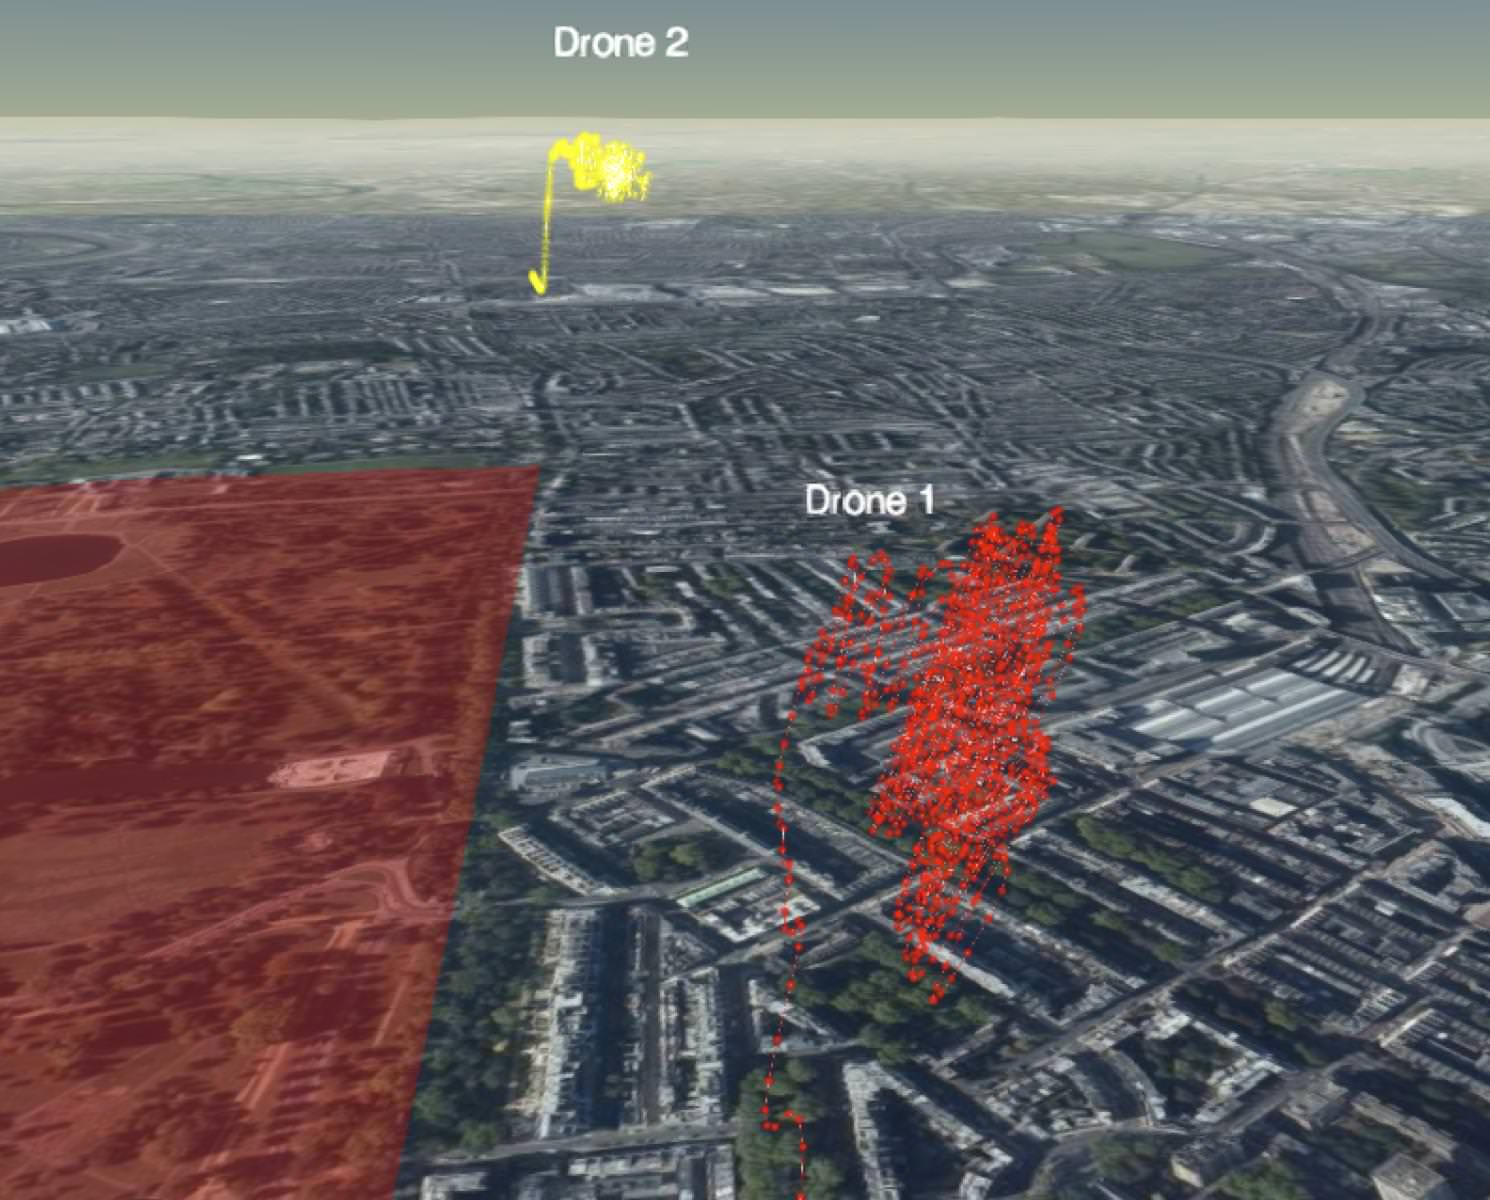
\includegraphics[width=\linewidth]{img/aatc_spaghett.jpg}
  \caption{Drone paths after increasing repulsion constant by 3 orders of magnitude.}
  \label{fig:aatc_spaghett}
\end{figure}

\newpage
Effectively, an initial range of values (see Table \ref{tab:gen_alg}) is provided and the genetic algorithm cycles through all of these, letting these constants compete against each other to see which set of constants produces the simulation with the lowest cost. This cost is determined from a cost function that returns the remaining battery life of a drone if it reaches its destination, or a relatively huge number otherwise.
$$cost = \sum_{testcase} \sum_{drone}
    \begin{cases}
      batteryUsed & if \; drone \; reached \; destination    \\
      100000 & otherwise \\

   \end{cases}$$

\begin{table}[!hbpt]
\centering
\begin{tabular}{|l|l|l|l|l|}
\hline
Constant           & Min & Max & Step & Total \\ \hline
Attraction         & 0.8 & 1.1 & 0.1    & 3     \\ \hline
Repulsion          & 100 & 500 & 100  & 5     \\ \hline
Return             & 0.1 & 0.7 & 0.2  & 4     \\ \hline
Influence distance & 300 & 600 & 100  & 4     \\ \hline
\multicolumn{4}{|l|}{Population}      & 240   \\ \hline
\end{tabular}
\caption{Initial configuration of the genetic algorithm for AATC. \cite{Balaji2017}}
\label{tab:gen_alg}
\end{table}

\subsection{Conclusions}
In the end, the genetic algorithms only improved the simulations by about 2\%\cite{Balaji2017} which could mean that the original range of constants was already a good set to work with. However, there is still scope for even greater improvements if the genetic algorithm was to be run with a greater number of test scenarios, bigger range of values to cycle through, and generally larger simulations.

\section{Scheduling Algorithms}
In this section we look at a few well known CPU scheduling algorithms\cite{Bell2018}. Although CPU scheduling is not part of this project, being able to understand a few different approaches to the problem will give insight into how to schedule drones later on. However, there are two key difference between drone and CPU scheduling.

\newpage
The first is that CPUs can time slice different tasks whereas once a drone is scheduled onto a task, it has to complete the whole task before being able to pick up a new one. Secondly, there are vastly more drones that could be running at a point in time compared to the number of cores in multi-core CPU, leading to far greater parallelism.

\subsection{First Come First Serve (FCFS)}
As the title says, this algorithm operates as a FIFO queue where tasks are scheduled in the same order that they arrive. Some might consider this the fairest form of scheduling, since it does not discriminate against any task, but simply prioritises the one that arrived soonest.

\subsection{Shortest Job First (SJF)}
This approach looks at the time each incoming task would take to complete, and puts the shortest task at the front of the schedule. While this means that small tasks get completed quickly, a constant stream of small tasks could mean that any heavier tasks never get scheduled or completed.

\subsection{Priority Scheduling}
Priority scheduling is a more general case of SJF, since each task is now given a priority - defined either internally or externally - and tasks with the highest priority are scheduled first. In SJF, the inverse of the estimated job time is used as the priority.

\subsection{Multi-Level Feedback Queue (MLFQ)}
MLFQ is an extension of an ordinary multi-level queue, where there are several queues of tasks to be completed and tasks are scheduled from non-empty queues in a round-robin fashion. A benefit of this approach is that each queue could be running different scheduling algorithms that better fits the priority of that queue.\\

\begin{figure}[!hbpt]
  \center
  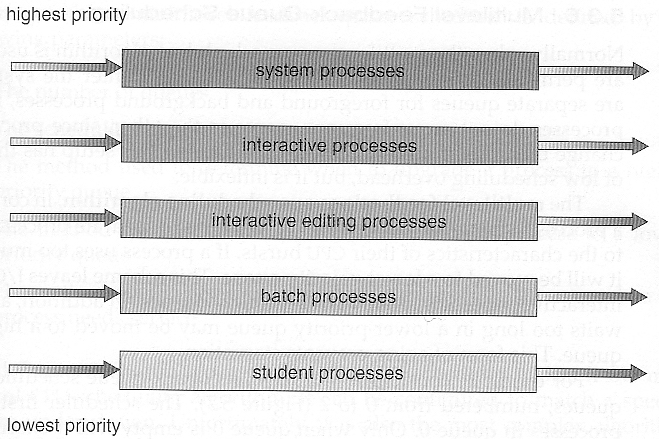
\includegraphics[width=0.6\linewidth]{img/mlqs.jpg}
  \caption{Multiple levels of queues, scheduled in a round-robin fashion. \cite{Bell2018}}
  \label{fig:mlqs}
\end{figure}

The ``feedback'' element of MLFQ allows tasks to be moved from one queue to another, depending on changes of circumstances. For example, if a queue has been left in a low priority queue for long enough, it may be moved to a higher priority queue - thus improving the chance that all incoming tasks get scheduled at some point in time.

\begin{figure}[!hbpt]
  \center
  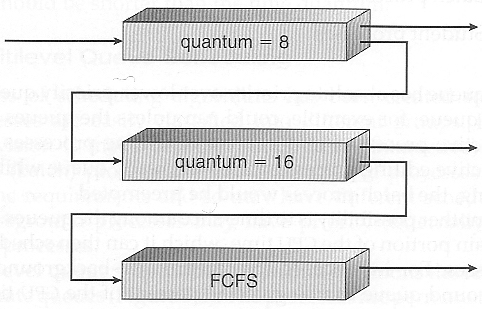
\includegraphics[width=0.6\linewidth]{img/mlfqs.jpg}
  \caption{Arrows indicate tasks can be moved up one queue to another. \cite{Bell2018}}
  \label{fig:mlfqs}
\end{figure}

\section{Time Value}
Thus far, we have shown that whilst there is great scope to utilise drones for delivery of physical goods, the existing implementation of AATC only touches upon the routing aspect - how to get from point A to point B. Even in all the test cases, the drones' start and end points were hand-picked by the developers\cite{Balaji2017} to give an insight into how AATC would operate in a variety of scenarios.\\

To gain greater understanding of how drones can positively impact industries, simulations need to be performed which take into account the financial aspect of their use case. For example when it comes to drone delivery networks, we want to ensure that the drones not only reach their destination quickly, but that they also get scheduled and utilised in the appropriate manner to maximise the profitability of the network.

\subsection{Time-Value of Money}
As described by Investopedia \cite{Investopedia}, the \textit{Time-Value of Money} is ``the concept that money available at the present time is worth more than the identical sum in the future due to its potential earning capacity''. This draws from the idea that investors would prefer to receive the same amount of money sooner rather than later, in order to obtain interest from the sum or reinvest it for greater growth.

\subsection{Time-Value of Data}
By a similar train of thought, there is the concept of the \textit{Time-Value of Data} - whereby the value to a business of some data decays over time and it is best to gain insight from it as soon as possible. This idea is often used in business intelligence, where companies may have large sets of unstructured data that need to be processed and analysed to derive value for the business. For example, a retailer would rather know what its users are interested in now rather than a month ago, so that they can tailor their sales and offers to leverage customer interest.

\newpage
\section{SpatialOS}
SpatialOS is a platform, created by \textit{Improbable}\cite{ImprobableWorldsLtd.2018a}, for running massive-scale simulated worlds. In their own words\cite{ImprobableWorldsLtd.2018b}:
\begin{displayquote}
SpatialOS is a cloud-based computational platform that lets you use many servers and engines to power a single world. The platform coordinates a swarm of micro-services called workers, which overlap and dynamically reorganize to power a huge, seamless world. The platform also lets you handle a huge number of concurrent players across different devices in one world.
\end{displayquote}

Although most commonly used for large distributed game worlds, SpatialOS has been used for simulating cities\cite{Narula2017}, the backbone of the Internet\cite{ImprobableWorldsLtd.2016} and a model of the brain\cite{ImprobableWorldsLtd.2018}. It is an ideal platform for simulating ``independent entities that have a location in space''\cite{ImprobableWorldsLtd.2018}.

\begin{figure}[!hbpt]
\centering
\begin{subfigure}{.5\textwidth}
  \centering
  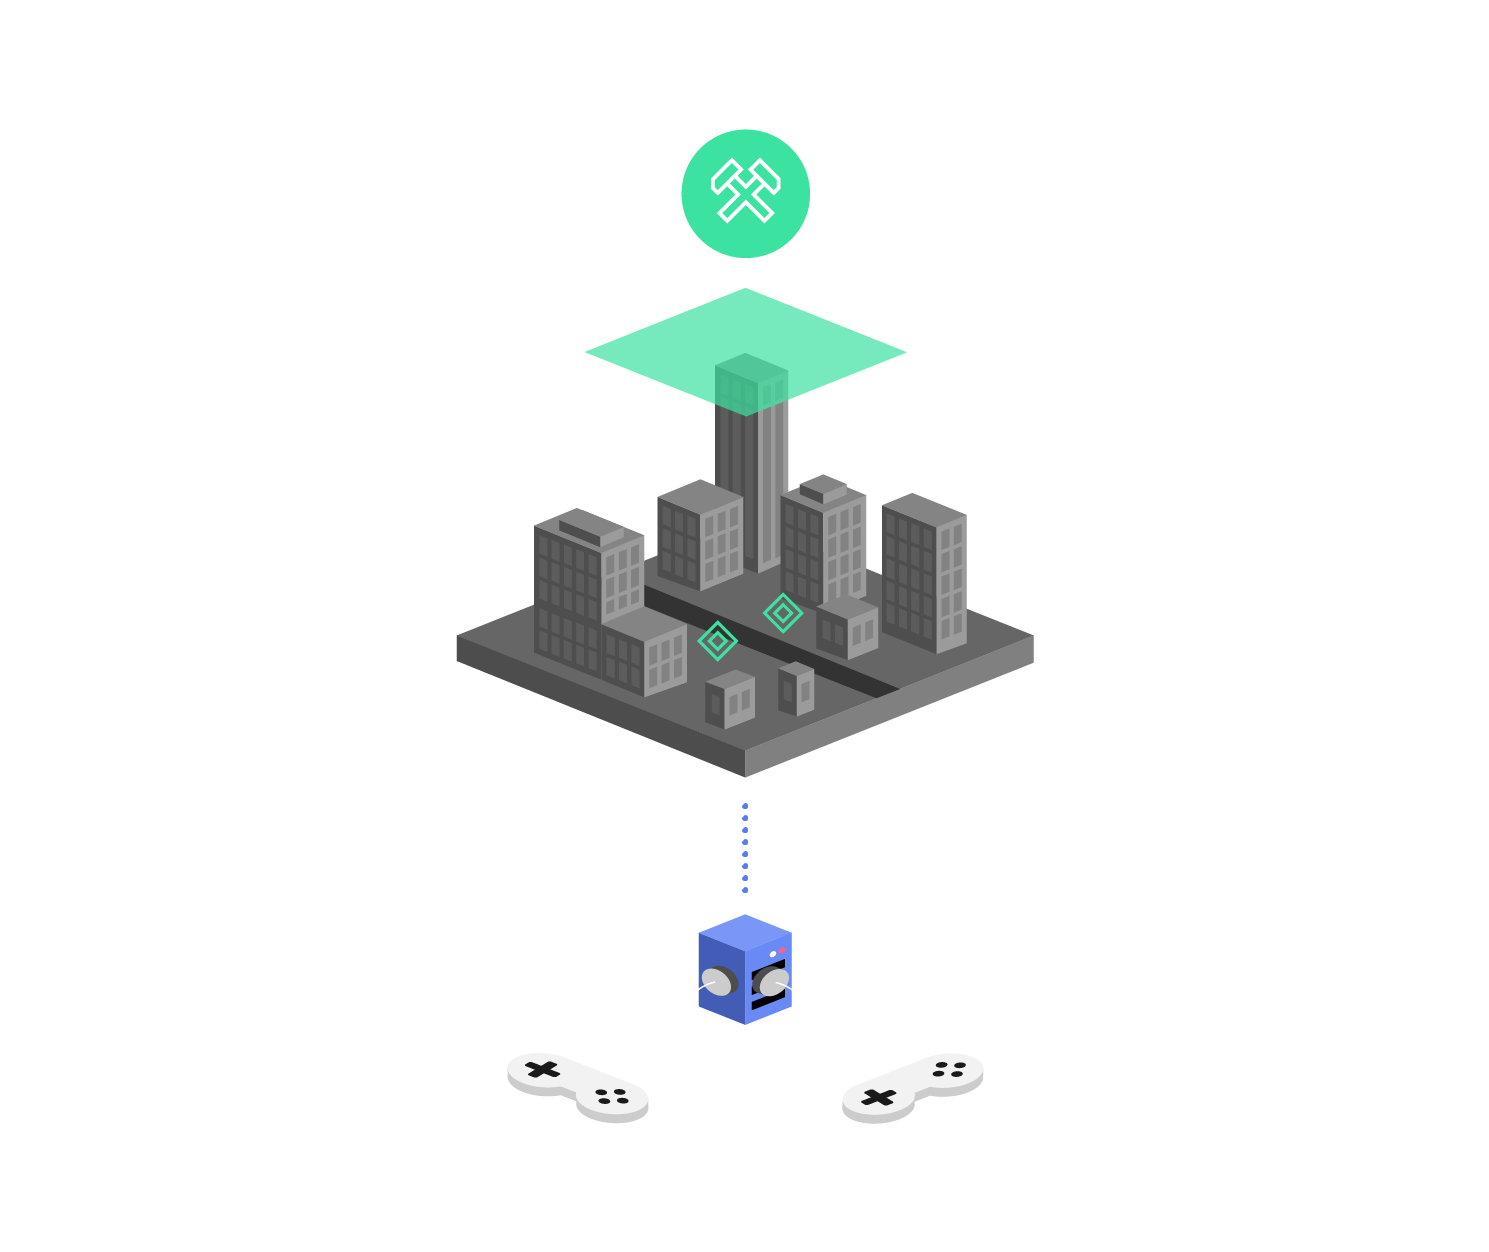
\includegraphics[width=\linewidth]{img/spatialos-diagram_current2.png}
  \caption{The current approach.}
  \label{fig:spatialos-diagram_current2}
\end{subfigure}%
\begin{subfigure}{.5\textwidth}
  \centering
  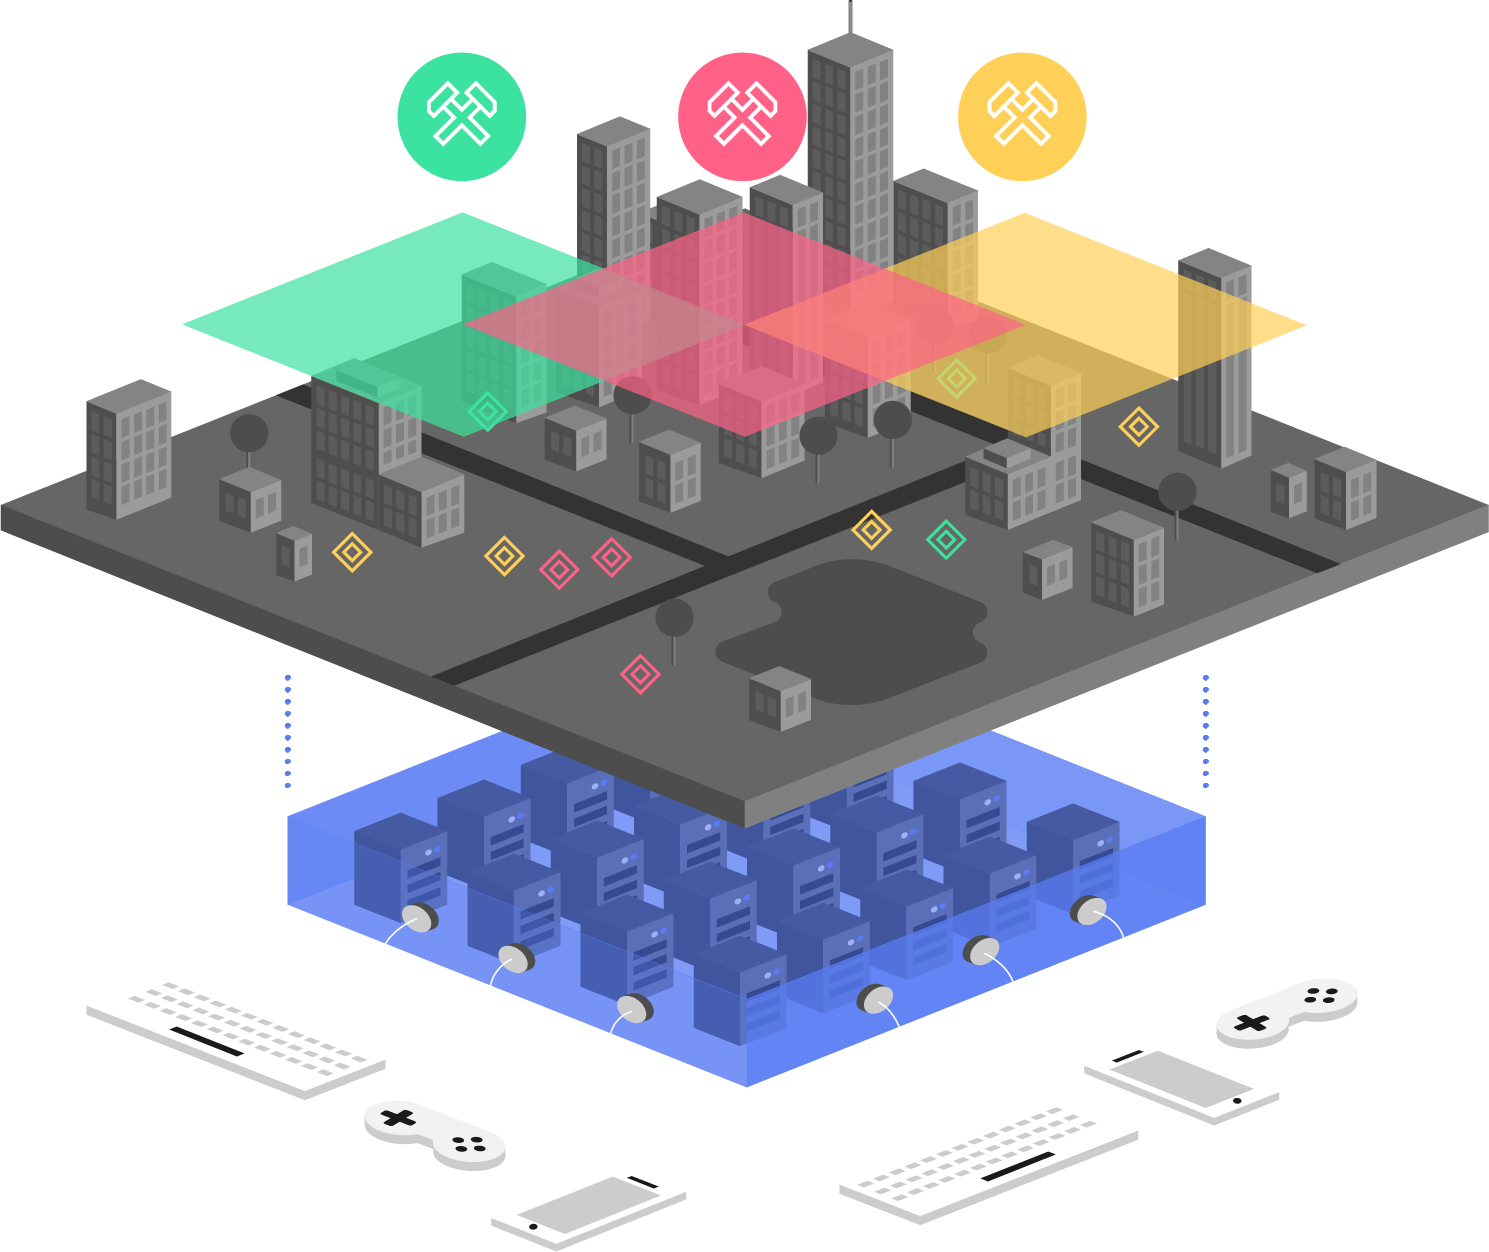
\includegraphics[width=\linewidth]{img/spatialos-diagram_solution2.png}
  \caption{How SpatialOS is different.}
  \label{fig:spatialos-diagram_solution2}
\end{subfigure}
\caption{Comparing approaches to multiplayer. \cite{ImprobableWorldsLtd.2018b}}
\label{fig:test}
\end{figure}

Anybody is able to sign up and use SpatialOS to build games using either the Unity3D or Unreal game engines. Alternatively, one can use the C\#, C++ and Java SDKs to create custom workers to be ran on SpatialOS deployments. \\

A benefit of SpatialOS's Unity and Unreal SDKs is that creating a sole game client, without manually writing network code, is almost enough to get multiplayer built-in to the game for ``free'', i.e. taken as granted.

\subsection{Unity SDK}
Of the two game engine integrations, the Unity SDK is arguably the most stable because it has been in development for far longer than the Unreal SDK, and it is not in beta. From prior industrial experience, the Unity integration is also easier to implement quick prototypes with and iterate on.

\subsection{Abstraction}
SpatialOS adopts an \textbf{Entity}-\textbf{Component}-\textbf{Worker} model.
\begin{itemize}
  \item \textbf{Entities} are anything in the world that have a position.
  \item \textbf{Components} define state and how other entities interact with them.
  \item \textbf{Workers} are micro-services that simulate components of entities in the world.
\end{itemize}

\subsection{Developer Tools}
There is extensive logging of performance metrics, which is a fantastic starting point for scaling up a simulation\cite{Brighting}. In addition to this, there is an active developer \textbf{Forum} - where SpatialOS developers and Improbable engineers meet to help other SDK users solve their problems\cite{ImprobableWorldsLtd.2018c}. \\

Naturally as the public SDKs have matured, so too have the public-facing developer tools. Currently, there is an \textbf{Inspector} to view the location of entities and the values that their components have at a given time, in either a local or deployed simulation.

\subsection{Layered Simulation}
By virtue of games having several dynamic systems all interlinking with each other, it is possible to create layered simulations on SpatialOS. This works well with the concept of Global, Reactive and Zonal layers that have been mentioned already in Sections 2.4, 2.5 and 2.6. Furthermore, as SpatialOS is distributed by nature, it is the ideal platform to create and execute massive, layered, distributed simulations.

\begin{figure}[!hbpt]
  \center
  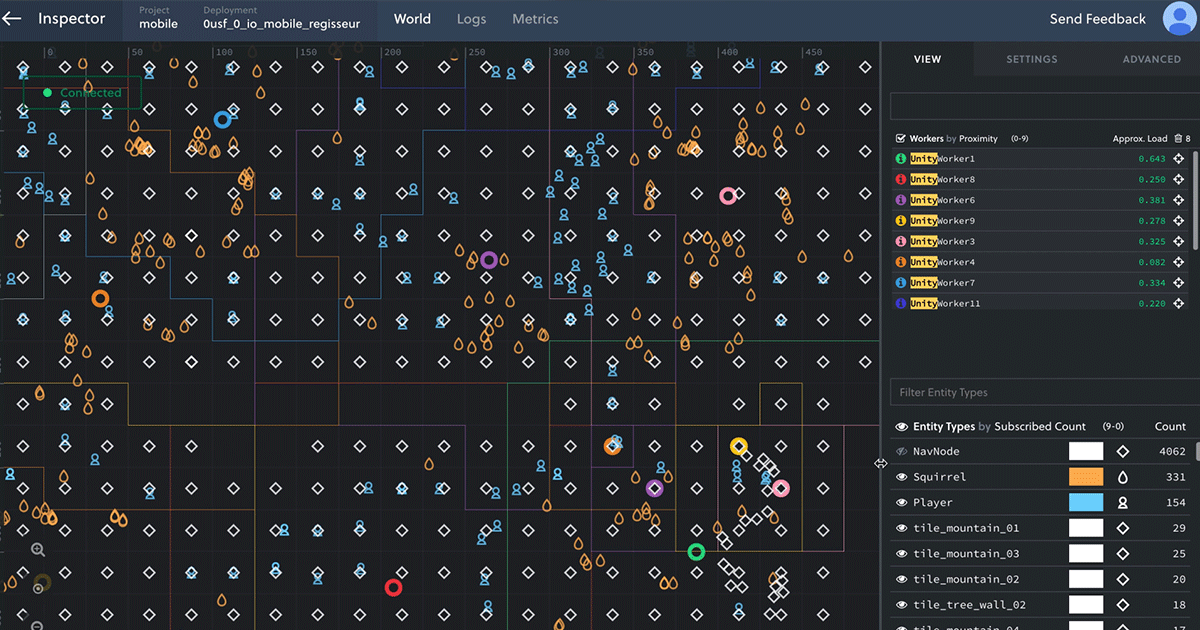
\includegraphics[width=\linewidth]{img/io_inspector.png}
  \caption{The Inspector demonstrating a deployment of the iOS Demo, \textit{Quest}. \cite{ImprobableWorldsLtd.2017}}
  \label{fig:bg_scalable_zones}
\end{figure}


%**********************************************%
\clearpage
\part{Skeleton Implementation}
\chapter{Translating AATC to SpatialOS}
Before even thinking about simulating orders and scheduling deliveries, there must be a backbone in place that allows drones to get from a start to end point. To this end, the pathfinding and collision avoidance capabilities of AATC (Sections 2.4-2.6) will be the backbone of the simulation.

\section{Basic Interaction Model}
However, AATC was designed as a simple master-slave system such that the server assumed total control over each drone in the system. To produce a scalable delivery network, modifications have to made that allows entities to be decoupled and not limited to the constraints imposed by the existing AATC model.

\subsection{Drones}
As a testament to hardware and software improvements over time, modern consumer drones are now fully capable of avoiding obstacles \cite{DJI} and navigating to GPS locations on their own \cite{DJIb}. By taking this into account we can have drones responsible for their own movement, leading to greater autonomy in the simulated delivery network, in turn enabling the system to scale up to bigger areas with vastly more drones than AATC.\\

In the AATC case, drones would have to ping the server every second to request a suggested velocity for the drone. This means that the controller would have to compute new velocities for every single drone it controls, every second.

\begin{figure}[!hbpt]
 \centering
 \begin{tikzpicture}[node distance = 2mm and 55mm]
 \node [box](sp)                {Drone};
 \node [box,right=of sp] (sc)   {Server};
 \draw ([yshift=3mm] sp.east) edge[-stealth] node[midway, above] {ping every second} ([yshift=3mm] sc.west) ;
 \draw [->] ([yshift=-3mm] sc.west) to ["updated velocity"] ([yshift=-3mm] sp.east);
 \end{tikzpicture}
 \caption{Drone-Server Interaction in AATC.}
 % \label{fig:test}
 \end{figure}

This is a lot of effort that can be offloaded to the drone such as in our proposed model, where we simply provide drones their next waypoint and let them navigate to it by themselves. The only pings to the server now would be to request a new waypoint or to retrieve an updated list of nearby static obstacles.\\

This new Drone-Controller dynamic means that drones need to be responsible for avoiding dynamic obstacles and other physical entities all by themselves.

 \begin{figure}[!hbpt]
  \centering
 \begin{tikzpicture}[node distance = 2mm and 55mm]
  \node [box](sp)                {Drone};
  \node [box,right=of sp] (sc)   {Controller};
  \draw [->] ([yshift=3mm] sp.east)  to ["ping for waypoint"] ([yshift=3mm] sc.west) ;
  \draw [->] ([yshift=-3mm] sc.west) to ["next waypoint"] ([yshift=-3mm] sp.east);
  \end{tikzpicture}
  \caption{Updated Drone-Controller Interaction.}
  % \label{fig:proposed_drone_controller_interaction}
  \end{figure}

Essentially, the AATC Reactive Layer has been split from the server and will now reside on each drone. The drone must periodically ping a controller for details of the nearest static obstacle, and combine this information with data from its own sensors in order to effectively avoid both static and dynamic obstacles.

\subsection{Controllers}
Much like an air traffic control tower, controllers exist as entities responsible for guiding drones in a particular region of the world. As the collision avoidance Reactive Layer will now run on the drones, the controller will be running the pathfinding Global Layer and keep a bitmap representation of the world.

\clearpage
Since drones only know about their next waypoint, it is the responsiblity of the controller to know which waypoint a drone last visited and to return the correct next waypoint when requested, which could involve checking if the drone is actually at the waypoint it claims to be at. The controller should also return information on the closest static obstacle to the drone at a given point.

\section{Representing Entities}
\subsection{Unity SDK}
As we are working with the SpatialOS Unity SDK, we must become familiar with the concept of a \textit{Prefab}, an asset type that can be used as a template to spawn new object instances. In addition to prefabs, \textit{MonoBehaviours} are scripts added as a prefab component that are then attached to an object instance of the prefab.\\

For our simulation it is immediately clear that we need to create Drone and Controller prefabs, as they are two entity types that will be interacting with each other. Even if they do not possess any physical or graphical components, they require representation in the simulated world.\\

A Drone prefab would require MonoBehaviours to handle movement and collision avoidance, whereas a Controller prefab will contain scripts to deal with waypoint management, pathfinding and world representation.

\subsection{SpatialOS Components}
SpatialOS, like many game engines, works as an Entity-Component-System (ECS). The way to define these the components that entities in the world can have is through the \textit{Schema}. The schema is used to generate code that can then be used by prefab scripts in order to update the SpatialOS state of objects.

\clearpage
Each component requires a unique, explicitly defined component ID to distinguish it from other components. Then optionally, we can define properties, events and commands. Properties hold the state of a component, events are used to trigger intra-entity actions, and commands are request-response operations that indicate how different entities communicate with each other.\\

\begin{sexylisting}[colback=white]{Example Schema - Health}
package improbable.example;

type DamageResponse {}
type DamageRequest {
  uint32 amount = 1;
}

component Health {
  id = 1234;
  uint32 health = 1;
  command DamageResponse damage(DamageRequest);
}
\end{sexylisting}

When spawning an entity, we create a \textit{template} of a defined prefab and add the components that we wish to be on that entity, setting the initial state of component properties in the process. In the case of a Health component we may wish to set \textit{health} of a player to 100, but 20 for little monsters and perhaps 200 for boss fights.\\

SpatialOS is then tasked with spawning an entity using the template, with the ability to set callbacks for both successful and failed creation attempts.\\

\begin{sexylisting}[colback=white]{Creating a Cube Template}
public static Entity CreateCubeTemplate()
{
  return EntityBuilder.Begin()
    .AddPositionComponent(...)
    .AddMetadataComponent(entityType: SimulationSettings.CubePrefabName)
    .SetPersistence(true)
    .SetReadAcl(...)
    .AddComponent(new Rotation.Data(...))
    .Build();
}
\end{sexylisting}

\begin{sexylisting}[colback=white]{Spawning a Cube Object}
var cubeTemplate = EntityTemplateFactory.CreateCubeTemplate();
SpatialOS.Commands.CreateEntity(PositionWriter, cubeTemplate)
  .OnSuccess((obj) =>
    Debug.LogFormat("Created Entity {0}", obj.createdEntityId))
  .OnFailure(() => Debug.LogError("Unable to spawn Cube."));
\end{sexylisting}

\newpage
\chapter{Implementation of Core Entities}
\section{Controller}
A Controller has three distinct components to it which all operate together, two of which are the Global Layer and corresponding Bitmap. A \textit{GridGlobalLayer} script would be used to generate a simple path from start to destination when requested. On initialisation, it would need to populate and update the Bitmap component with details of all the No Fly Zones in the that controller's region of the world.\\

\textit{GridGlobalLayer} itself will be called by \textit{ControllerBehaviour}. This MonoBehaviour is responsible for overseeing the overall operation of a Controller. Spawning drones, calling the pathfinding component, and updating the drone-waypoint mappings are all examples of tasks that this "master" behaviour would have to handle.\\

Figure \ref{fig:controller_global_bitmap_flow} describes how the three components slot next to each other, each performing its own set of tasks but maintaining separation of logic and state.

\begin{figure}[!hbpt]
 \centering
 \begin{tikzpicture}[node distance = 2cm, auto]
     % Place nodes
     \node [block] (controller) {Controller Behaviour};
     % \node [cloud, right of=controller, node distance=5cm] (genpath) {Generate Path};
     \node [block, below of=controller, node distance=3cm] (globallayer) {Global Layer};
     % \node [cloud, left of=globallayer, node distance=5cm] (checknfz) {Check No Fly Zones};
     \node [block, below of=globallayer, node distance=3cm] (bitmap) {Bitmap};
     % \node [cloud, left of=init] (expert) {expert};
     % \node [cloud, right of=init] (system) {system};
     % \node [block, below of=init] (identify) {identify candidate models};
     % \node [block, below of=identify] (evaluate) {evaluate candidate models};
     % \node [block, left of=evaluate, node distance=3cm] (update) {update model};
     % \node [decision, below of=evaluate] (decide) {is best candidate better?};
     % \node [block, below of=decide, node distance=3cm] (stop) {stop};
     % Draw edges
     \path [line] (controller) -- node {Pathfinding Request} (globallayer);
     % \path [line] (genpath) -- (globallayer);
     \path [line] (globallayer) -- node {World Map Lookups} (bitmap);
     \path [line] (bitmap) -- (globallayer);
     % \path [line] (identify) -- (evaluate);
     % \path [line] (evaluate) -- (decide);
     % \path [line] (decide) -| node [near start] {yes} (update);
     % \path [line] (update) |- (identify);
     % \path [line] (decide) -- node {no}(stop);
     % \path [line,dashed] (expert) -- (init);
     % \path [line,dashed] (system) -- (init);
     % \path [line,dashed] (system) |- (evaluate);
 \end{tikzpicture}
 \caption{Example Component Flow.}
 \label{fig:controller_global_bitmap_flow}
 \end{figure}

\subsection{No Fly Zones}
No Fly Zones are represented in a similar way to AATC, as a list of float vectors with two vectors to track opposing corners of the zone's bounding box. An initial list of No Fly Zones is passed into the Global Layer upon creation of the component, with scope to add and remove from the list if one so wishes.\\
\begin{sexylisting}[colback=white]{NoFlyZone Schema Type}
type NoFlyZone {
  improbable.Vector3f bounding_box_bottom_left = 1;
  improbable.Vector3f bounding_box_top_right = 2;
  list<improbable.Vector3f> vertices = 3;
}
\end{sexylisting}

To complement the C\# class that SpatialOS generates from this, we have implemented a static class (Appendix A.1) containing methods that are necessary for integrating No Fly Zones with the Global Layer and Bitmap components. These are checks to see if:
\begin{itemize}
  \item a given point is within a zone's bounding box
  \item a given point is within a zone's polygonal area
  \item a given point is within any zone from a given list
\end{itemize}

\clearpage
\subsection{Pathfinding and Waypoints}
Once the No Fly Zone data is initialised, it is the controller's job to generate a list of NFZ-avoiding waypoints that a drone will follow to get from start to destination. The controller needs to maintain a list of waypoints for each drone, as well as the next waypoint that each drone will need to go to.\\

This is achieved by keeping a mapping of a drone's ID to it's DroneInfo type, which contains a list of waypoints and the index of the last sent waypoint.\\

When a drone reaches a waypoint it calls the \textit{request\_new\_target} command on its assigned controller, which then locates the DroneInfo of said drone. The \textit{next\_waypoint} field is incremented and the next waypoint is subsequently found and returned to the drone. If the field value is greater than or equal to the length of the list, the drone has clearly reached the final waypoint, its ultimate destination.

\begin{sexylisting}[colback=white]{Basic Controller Schema}
enum TargetResponseCode {
  SUCCESS = 0;
  WRONG_CONTROLLER = 1;
  JOURNEY_COMPLETE = 2;
}

type TargetRequest {
  EntityId drone_id = 1;
}

type TargetResponse {
  improbable.Vector3f new_target = 1;
  TargetResponseCode success = 2;
}

type DroneInfo {
  int32 next_waypoint = 1;
  list<improbable.Vector3f> waypoints = 2;
}

component Controller {
  id = 1200;
  uint32 max_drone_count = 2;
  map<EntityId, DroneInfo> deliveries_map = 3;
  bool initialised = 4;
  Vector3f top_left = 5;
  Vector3f bottom_right = 6;
  command TargetResponse request_new_target(TargetRequest);
}
\end{sexylisting}

\clearpage
\subsection{World Bitmap}
In the original AATC implementation, the bitmap was represented as a byte array with each cell representing a 25m x 25m area of the world. Since the only information stored in the bitmap is the presence and proximity to NFZs, the array is sparse and therefore better represented as a map from cell number to GridType.\\

\begin{sexylisting}[colback=white]{Bitmap Component and GridType Enum}
enum GridType {
  OUT = 0;
  IN = 1;
  NEAR = 2;
}

component BitmapComponent {
  id = 1204;
  improbable.Vector3f top_left = 1;
  improbable.Vector3f bottom_right = 2;
  int32 width = 3;
  int32 height = 4;
  int32 grid_width = 7;
  int32 grid_height = 8;
  map<int32, GridType> grid = 5;
  bool initialised = 6;
}
\end{sexylisting}

\clearpage
The benefit of this implementation is that only relevant data is stored in the map, with failure to find a cell in the map implying that the corresponding area of the world is not in or near a No Fly Zone. Since every controller will have a Bitmap component, this design improves memory efficiency and provides more options to the controller. It could simply reduce its memory footprint, deal with larger areas, or reduce the cell size to represent the world with a higher precision.

\subsection{Assisting the Reactive Layer}
Although collision avoidance runs on the drone, it can not do the job properly without knowing the closest point to it on a NFZ. This is where the controller comes in and asks the bitmap to return the closest NFZ point. Since NFZs extend across all altitudes, the drone's altitude is used as the y-coordinate of the closest NFZ point.\\

This means that there is now a fourth component to the Controller entity, existing just to deal with requests from drones for the nearest static obstacle. This is shown as the \textit{get\_nearest\_obstacle} command, which returns the \textit{APFObstacle} used by drone-side collision avoidance code.\\

\begin{sexylisting}[colback=white]{Reactive Layer Request Handler}
void GetNearestObstacle(RequestHandle handle)
{
  Vector3f nfz = bitmap.nearestNFZPoint(handle.Request.location);
  APFObstacleType type = APFObstacleType.NO_FLY_ZONE;
  if (nearestNoFlyZone.y < 0)
  {
    type = APFObstacleType.NONE;
  }
  handle.Respond(new ObstacleResponse(new APFObstacle(type, nfz)));
}
\end{sexylisting}

\begin{sexylisting}[colback=white]{Reactive Layer Schema}
package improbable.drone;

import "improbable/vector3.schema";

enum APFObstacleType {
  NONE = 0;
  MANNED_AVIATION = 1;
  DRONE = 2;
  NO_FLY_ZONE = 3;
  HIDDEN_OBSTACLE = 4;
}

type APFObstacle{
  APFObstacleType type = 1;
  improbable.Vector3f position = 2;
}

type ObstacleRequest {
  improbable.Vector3f location = 1;
}

type ObstacleResponse {
  APFObstacle obstacle = 1;
}

component ReactiveLayer {
  id = 1205;
  command ObstacleResponse get_nearest_obstacle(ObstacleRequest);
}
\end{sexylisting}

\subsection{Drone Spawning}
For simplicity at this early stage, controllers just generate a path between two random non-NFZ points in the world. They spawn a drone at the first random point and de-spawn each drone once it reaches its final waypoint. For testing purposes collisions were initially disabled as the drones just blindly moved from waypoint to waypoint without any collision avoidance.

\begin{figure}[!hbpt]
  \center
  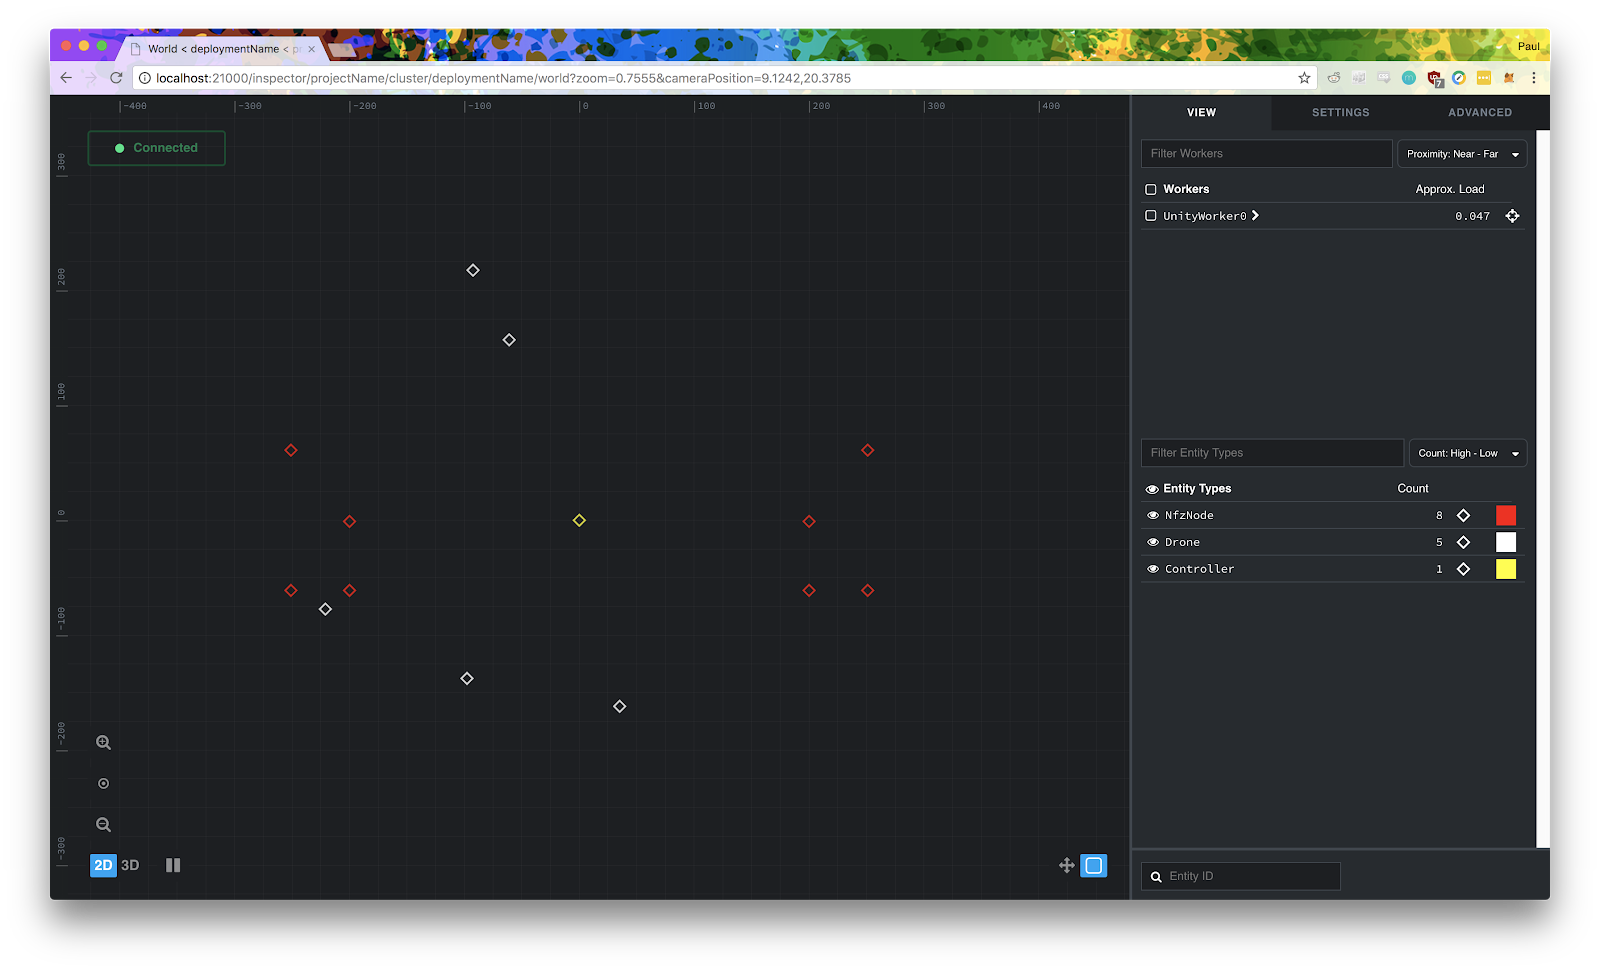
\includegraphics[width=\linewidth]{img/gdoc1.png}
  \caption{Testing basic controller functionality.}
  \label{fig:basic_controller_test}
\end{figure}

In Figure \ref{fig:basic_controller_test}, we check if the controller returns correct waypoints in order by spawning drones either side of the NFZ and observing if the flight path avoids the obstacle.

\section{Drone}
Compared to a controller, a drone is a far less complex entity. It has one main component to maintain state of the drone's next waypoint, current direction, target request status, and maximum speed. The core loop of the \textit{DroneBehaviour} script executes every second, updating SpatialOS with the drone position and then either recalculating direction or requesting a new target, depending on the drone's status.

\begin{sexylisting}[colback=white]{Main Drone Loop (once a second)}
void DroneTick()
{
  if (simulate)
  {
    SendPositionUpdate();
    if (DroneDataWriter.Data.droneStatus == DroneStatus.MOVE)
    {
      apf.Recalculate();
    }
    if (DroneDataWriter.Data.targetPending == TargetPending.WAITING)
    {
      requestNewTarget();
    }
    float distanceToTarget = Vector3.Distance(target, transform.position);
    if (DroneDataWriter.Data.targetPending == TargetPending.REQUEST
      || distanceToTarget < radius)
    {
      requestNewTarget();
    }
  }
}
\end{sexylisting}

Actual movement of the drone occurs in a separate method (Listing 10) \textit{four} times a second. This is done so that the drones visually appear to move smoother and the separation exists to reduce how often we perform the costly tasks of detecting and avoiding nearby drones.\\

Adding this separation will also make it easier down the road when we introduce energy consumption to the drones, because we can then simply switch on the drone status to adjust how much energy has been consumed in the previous time frame. For example, a moving drone will consume more energy than a hovering drone.

\begin{sexylisting}[colback=white]{Drone Movement (four times a second)}
void MoveDrone()
{
  if (simulate)
  {
    if (DroneDataWriter.Data.droneStatus == DroneStatus.MOVE)
    {
      transform.position += direction * DroneDataWriter.Data.speed
        * SimulationSettings.DroneMoveInterval;
    }
  }
}
\end{sexylisting}

\subsection{Drone Detection}
In AATC the server knew the location of every drone in the world, which meant that searching for nearby drones would just be a case of iterating through the list of drones and finding the closest one. However, with SpatialOS we delegate this responsiblity to the drones.\\

The naive method would be for each drone to request all SpatialOS entities within a certain radius, and then filtering to find the closest one. The problem with this is that Spatial find queries are extremely expensive as they have to propagate up to the server instance, be executed, and then returned down to individual entities. In a world with 30 drones where each drone is recalculating its direction every second, that's 30 queries that have to be dealt with in tandem every second.\\

Due to the fact that each distributed ``worker'' in SpatialOS is an instance of the Unity game engine, a more practical approach is instead to utilise the engine and perform a simple physics collision check.

\clearpage
Although this is still resource-expensive, it is still quicker than a Spatial search because using native game engine functionality is more performant than manually searching for entities in a radius. By applying a Sphere Collider to each drone, checking for nearby colliders will only ever return instances of drones (Appendix A.2).

\subsection{Collision Detection}
Now that drones are detected easily, a collision is simply the case where a nearby collider is at a distance of less than 1m (2 drone radiuses). In the real world, a controller would detect that two drones have stopped responding and assume a crash occured. For our simulation, we instead add a command for drones to call so the controller knows a collision occurred. \\

\begin{sexylisting}[colback=white]{Reporting a Collision}
type CollisionResponse {}
type CollisionRequest {
  EntityId drone_id = 1;
  EntityId collider_id = 2;
}

command CollisionResponse collision(CollisionRequest);
\end{sexylisting}

Upon successful receipt of a \textit{CollisionRequest}, a controller may then destroy the drone instances to signal that they are not part of the system anymore. Looking ahead, the controller may decide to use this as a trigger to dispatch drone recovery services or apply penalties for crashing drones.

\section{Summary}
Now that the Drone and Controller entities have been created and relevant components added, we are able to create drones, send them between random locations, and destroy them upon journey completion.


%**********************************************%
\newpage
\chapter{Delivery Network Architecture}
As SpatialOS abstracts away all server-to-server connections and raw networking, we can consider any size world as one singular simulation. As explored thus far, our work only needs to go as far as the definition entities and how their components interact with each other. Since pathfinding and drone-controller communication channels have been set up and tested, our efforts now turn to upgrading this system into a scalable, distributed, delivery network.

\section{Delivery Destinations}
As per the current design, controllers spawn drones, generate a path between two points and then sequentially provide waypoints the drone should follow to get to its destination. To modify this for a delivery network case, the points should correspond to the locations of the controller and the delivery end point. As controllers are both stationary and responsible for pathfinding, making this change is trivial. The question now: how do controllers find out where the delivery end points are?\\

To resolve this we introduce an Order Generation entity to the simulation, whose sole functionality is to simulate a stream of delivery requests and route these requests to the appropriate controller. The Order Generator may eventually have a load balancing component to it in the future, but for now we simply route each delivery request to the controller closest to the package destination.\\

Figure \ref{fig:delivery_network_overview} shows how the Order Generator fits into the existing model. While controllers and drones represent physical things that will exist in the real world, order generation is a virtual entity that only exists for the purposes of the simulation. If such a system were to go live, the order generation entity would be replaced by the actual stream of orders that real customers would be placing.

\begin{figure}[!hbpt]
 \centering
 \begin{tikzpicture}[node distance = 2cm, auto]
     % Place nodes
     \node [block] (ordergeneration) {Order Generator};
     \node [block, below of=ordergeneration, node distance=3cm] (controller1) {Controller};
     \node [block, left of=controller1, node distance=3cm] (controller2) {Controller};
     \node [block, right of=controller1, node distance=3cm] (controller3) {Controller};
     \node [cloud, below of=controller1, node distance=2cm] (drone1) {Drones};
     \node [cloud, below of=controller2, node distance=2cm] (drone2) {Drones};
     \node [cloud, below of=controller3, node distance=2cm] (drone3) {Drones};
     % \node [cloud, left of=globallayer, node distance=5cm] (checknfz) {Check No Fly Zones};
     % \node [block, below of=checknfz, node distance=3cm] (bitmap) {Bitmap};
     % \node [cloud, left of=init] (expert) {expert};
     % \node [cloud, right of=init] (system) {system};
     % \node [block, below of=init] (identify) {identify candidate models};
     % \node [block, below of=identify] (evaluate) {evaluate candidate models};
     % \node [block, left of=evaluate, node distance=3cm] (update) {update model};
     % \node [decision, below of=evaluate] (decide) {is best candidate better?};
     % \node [block, below of=decide, node distance=3cm] (stop) {stop};
     % Draw edges
     \path [line] (ordergeneration) -- (controller1);
     \path [line] (ordergeneration) -- (controller2);
     \path [line] (ordergeneration) -- (controller3);
     \path [line] (controller1) -- (drone1);
     \path [line] (drone1) -- (controller1);
     \path [line] (controller2) -- (drone2);
     \path [line] (drone2) -- (controller2);
     \path [line] (controller3) -- (drone3);
     \path [line] (drone3) -- (controller3);
     % \path [line] (genpath) -- (globallayer);
     % \path [line] (globallayer) -- (checknfz);
     % \path [line] (checknfz) -- (bitmap);
     % \path [line] (identify) -- (evaluate);
     % \path [line] (evaluate) -- (decide);
     % \path [line] (decide) -| node [near start] {yes} (update);
     % \path [line] (update) |- (identify);
     % \path [line] (decide) -- node {no}(stop);
     % \path [line,dashed] (expert) -- (init);
     % \path [line,dashed] (system) -- (init);
     % \path [line,dashed] (system) |- (evaluate);
 \end{tikzpicture}
 \caption{Delivery Network Flow.}
 \label{fig:delivery_network_overview}
 \end{figure}

\section{Basic Order Generation}
Before generating any orders, we must first define the components on the Order Generator and Controller that deal with the sending and receiving of delivery requests.

\subsection{Delivery Handler / Scheduler}
Controllers will need a \textit{DeliveryHandler} component to enqueue incoming delivery requests. It follows that there are a finite amount of drones available to deliver goods at a particular point in time, therefore the Delivery Handler's function is to maintain a queue of requests and only provide the next delivery to serve when the \textit{ControllerBehaviour} asks for it. For the time being, we implement a very basic FIFO queue to serve requests in the order that they were received by the Controller.

\clearpage
The delivery handler effectively acts as a scheduler for the controller, because it decides the order to return requests in a manner completely transparent to core controller operation. The main loop (Appendix A.3) now checks if the controller can deploy a drone, asks for the next request, handles the delivery request if the scheduler returns one back, and sends the updated queue state up to SpatialOS.\\

To match up with this functionality the schema defines four basic elements:
\begin{enumerate}
  \item \textit{DeliveryRequest} type
  \item \textit{QueueEntry} type
  \item list of QueueEntry items
  \item \textit{request\_delivery} command
\end{enumerate}

\begin{sexylisting}[colback=white]{Delivery Handler Schema}
type DeliveryResponse {
  bool success = 1;
}

type DeliveryRequest {
  improbable.Vector3f destination = 1;
}

type QueueEntry {
  float timestamp = 1;
  DeliveryRequest request = 2;
}

component DeliveryHandler {
  id = 1201;
  list<QueueEntry> request_queue = 1;
  command DeliveryResponse request_delivery(DeliveryRequest);
}
\end{sexylisting}

We designed it this way so that \textit{DeliveryRequest} data could be extended later if we so wish. Important information about a delivery that will extend to support in the future include package weights, package types and even the priority of said delivery. Being able to extend the \textit{QueueEntry} also may open the door for us to play with more complex scheduling algorithms down the line.

\subsection{Order Generator}
Now that we have defined a basic \textit{DeliveryRequest} type, it is the order generator's job to regularly create and send these requests to the appropriate controller. At the moment the request only requires a location vector, so our plan to do this is to generate a random point in the world not in a No Fly Zone, and then find the closest controller to said point.\\

We would like the orders to be generated at regular time intervals such that each Controller receives an order every 30 seconds on average. By distributing controllers evenly such that each one is responsible for similar sized regions of the world, we can infer that the Order Generator works generates requests every $\frac{30}{\#controllers}$ seconds.\\

\begin{sexylisting}[colback=white]{Order Generator Schema}
type ControllerInfo {
  EntityId controller_id = 1;
  improbable.Vector3f location = 2;
}

component OrderGeneratorComponent {
  id = 1300;
  list<improbable.controller.NoFlyZone> zones = 1;
  list<ControllerInfo> controllers = 2;
}
\end{sexylisting}

\clearpage
In order to generate valid requests, we need to know about all the No Fly Zones in the world as well as the location and EntityId of each Controller. Since each controller will be placed at pre-determined locations from a starting snapshot, we know both of these details at snapshot-creation and can subsequently use this to set the starting state of the Order Generator.

\part{Incorporating Reality}
\chapter{Achieving London-Scale Simulation}
A snapshot represents the state of a simulated world at a point in time, storing each entity as well as each component's properties. Every deployment, both local and in the cloud, requires a starting snapshot to populate the simulation. To speed up this process, we create a \textit{scene} for snapshot generation and utilise the power of Unity Editor scripts to programmatically generate and modify snapshots with ease.

\begin{figure}[!hbpt]
  \center
  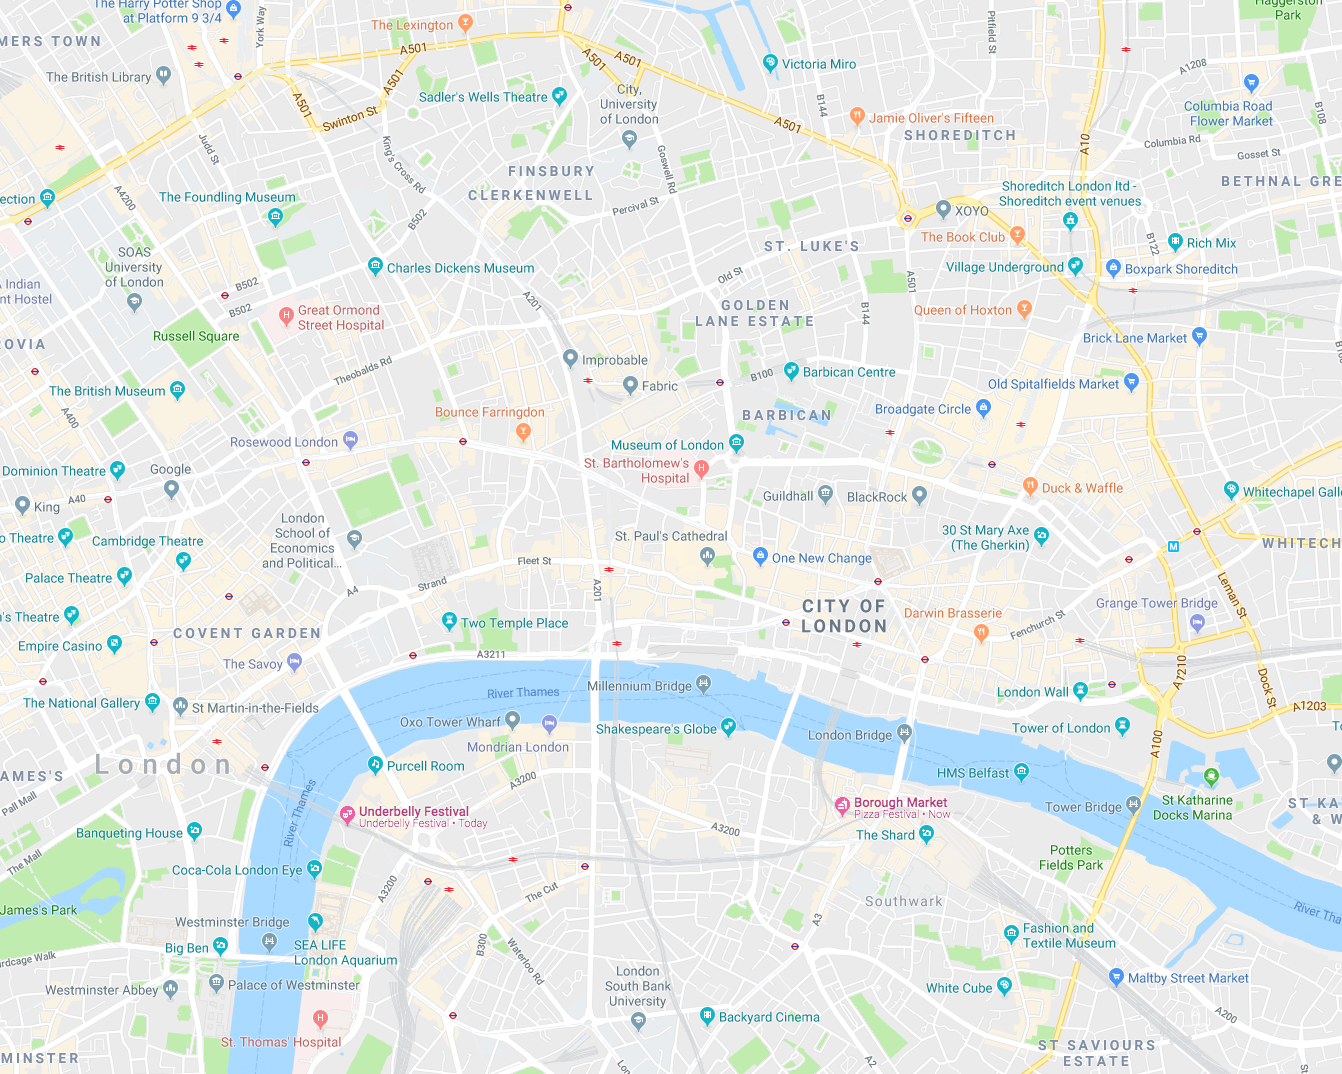
\includegraphics[width=0.9\linewidth]{img/london_snapshot_small.png}
  \caption{Our selected region of London. \cite{Google2018a}}
  \label{fig:london_snapshot_small}
\end{figure}

\section{Area Selection}
London was chosen as the city to simulate partly because of our geographical understanding but also because it could be a prime candidate for rolling out drone delivery services to. Traffic jams, congestion charges and fuel consumption are all ever-present issues for existing delivery networks. As the technology develops, being able to avoid and mitigate these issues by taking to the skies is a leap of faith many operators may be seriously considering.\\

In the spirit of walking before running, we opt to limit ourselves to a 5km x 4km region of central London, of which 4.8km x 3.8km is actually simulated. We wish to include a 100m wide border to avoid invoking (literal) edge cases in SpatialOS that may arise by simulating entites right at the boundaries of the world.\\

This particular part of London was chosen due to the variety of institutions and types of land there are available. There are parks, hospitals and skyscrapers that may be potentially protected by No Fly Zones, but there are also educational institutions either side of the river that could serve as ideal locations for Controllers if a pilot was commissioned.\\

Another major benefit to choosing this area of London is extensibility. Should we decide to, we have the ability to increase the size of the world to test the scalability of the system, adding more of the city and surrounding suburbia to the simulation.

\section{Snapshot Scene}
Figure \ref{fig:unity_londonsnapshotsmallexample} shows how the London scene looks in Unity when visually editing a snapshot. The leftmost column is known as the \textit{Hierarchy}, a list of all the objects currently in the scene. As we are able to nest objects, adding empty game objects allow one to group objects together. For example, No Fly Zones and Controllers could be nested in different groups to more easily distinguish the type of each object.

\clearpage
To the side of the Hierarchy is the \textit{Inspector}, which shows all the Unity components on a selected prefab, in this case a Drone. You may notice an additional component that we have not previously covered residing on this prefab.\\

Entities that are active and likely to be moving around the world need a special component called a \textit{Transform Receiver}, which simply updates the object's world position whenever its Spatial position is updated.

As each component is authoritative on exclusively the client or server, a completely server-side simulation (such as ours is at present) would require a \textit{Transform Receiver} to ensure that objects are receiving and applying the appropriate Spatial updates if we decide to implement a client-side simulation viewer in the future.

\begin{figure}[!hbpt]
  \center
  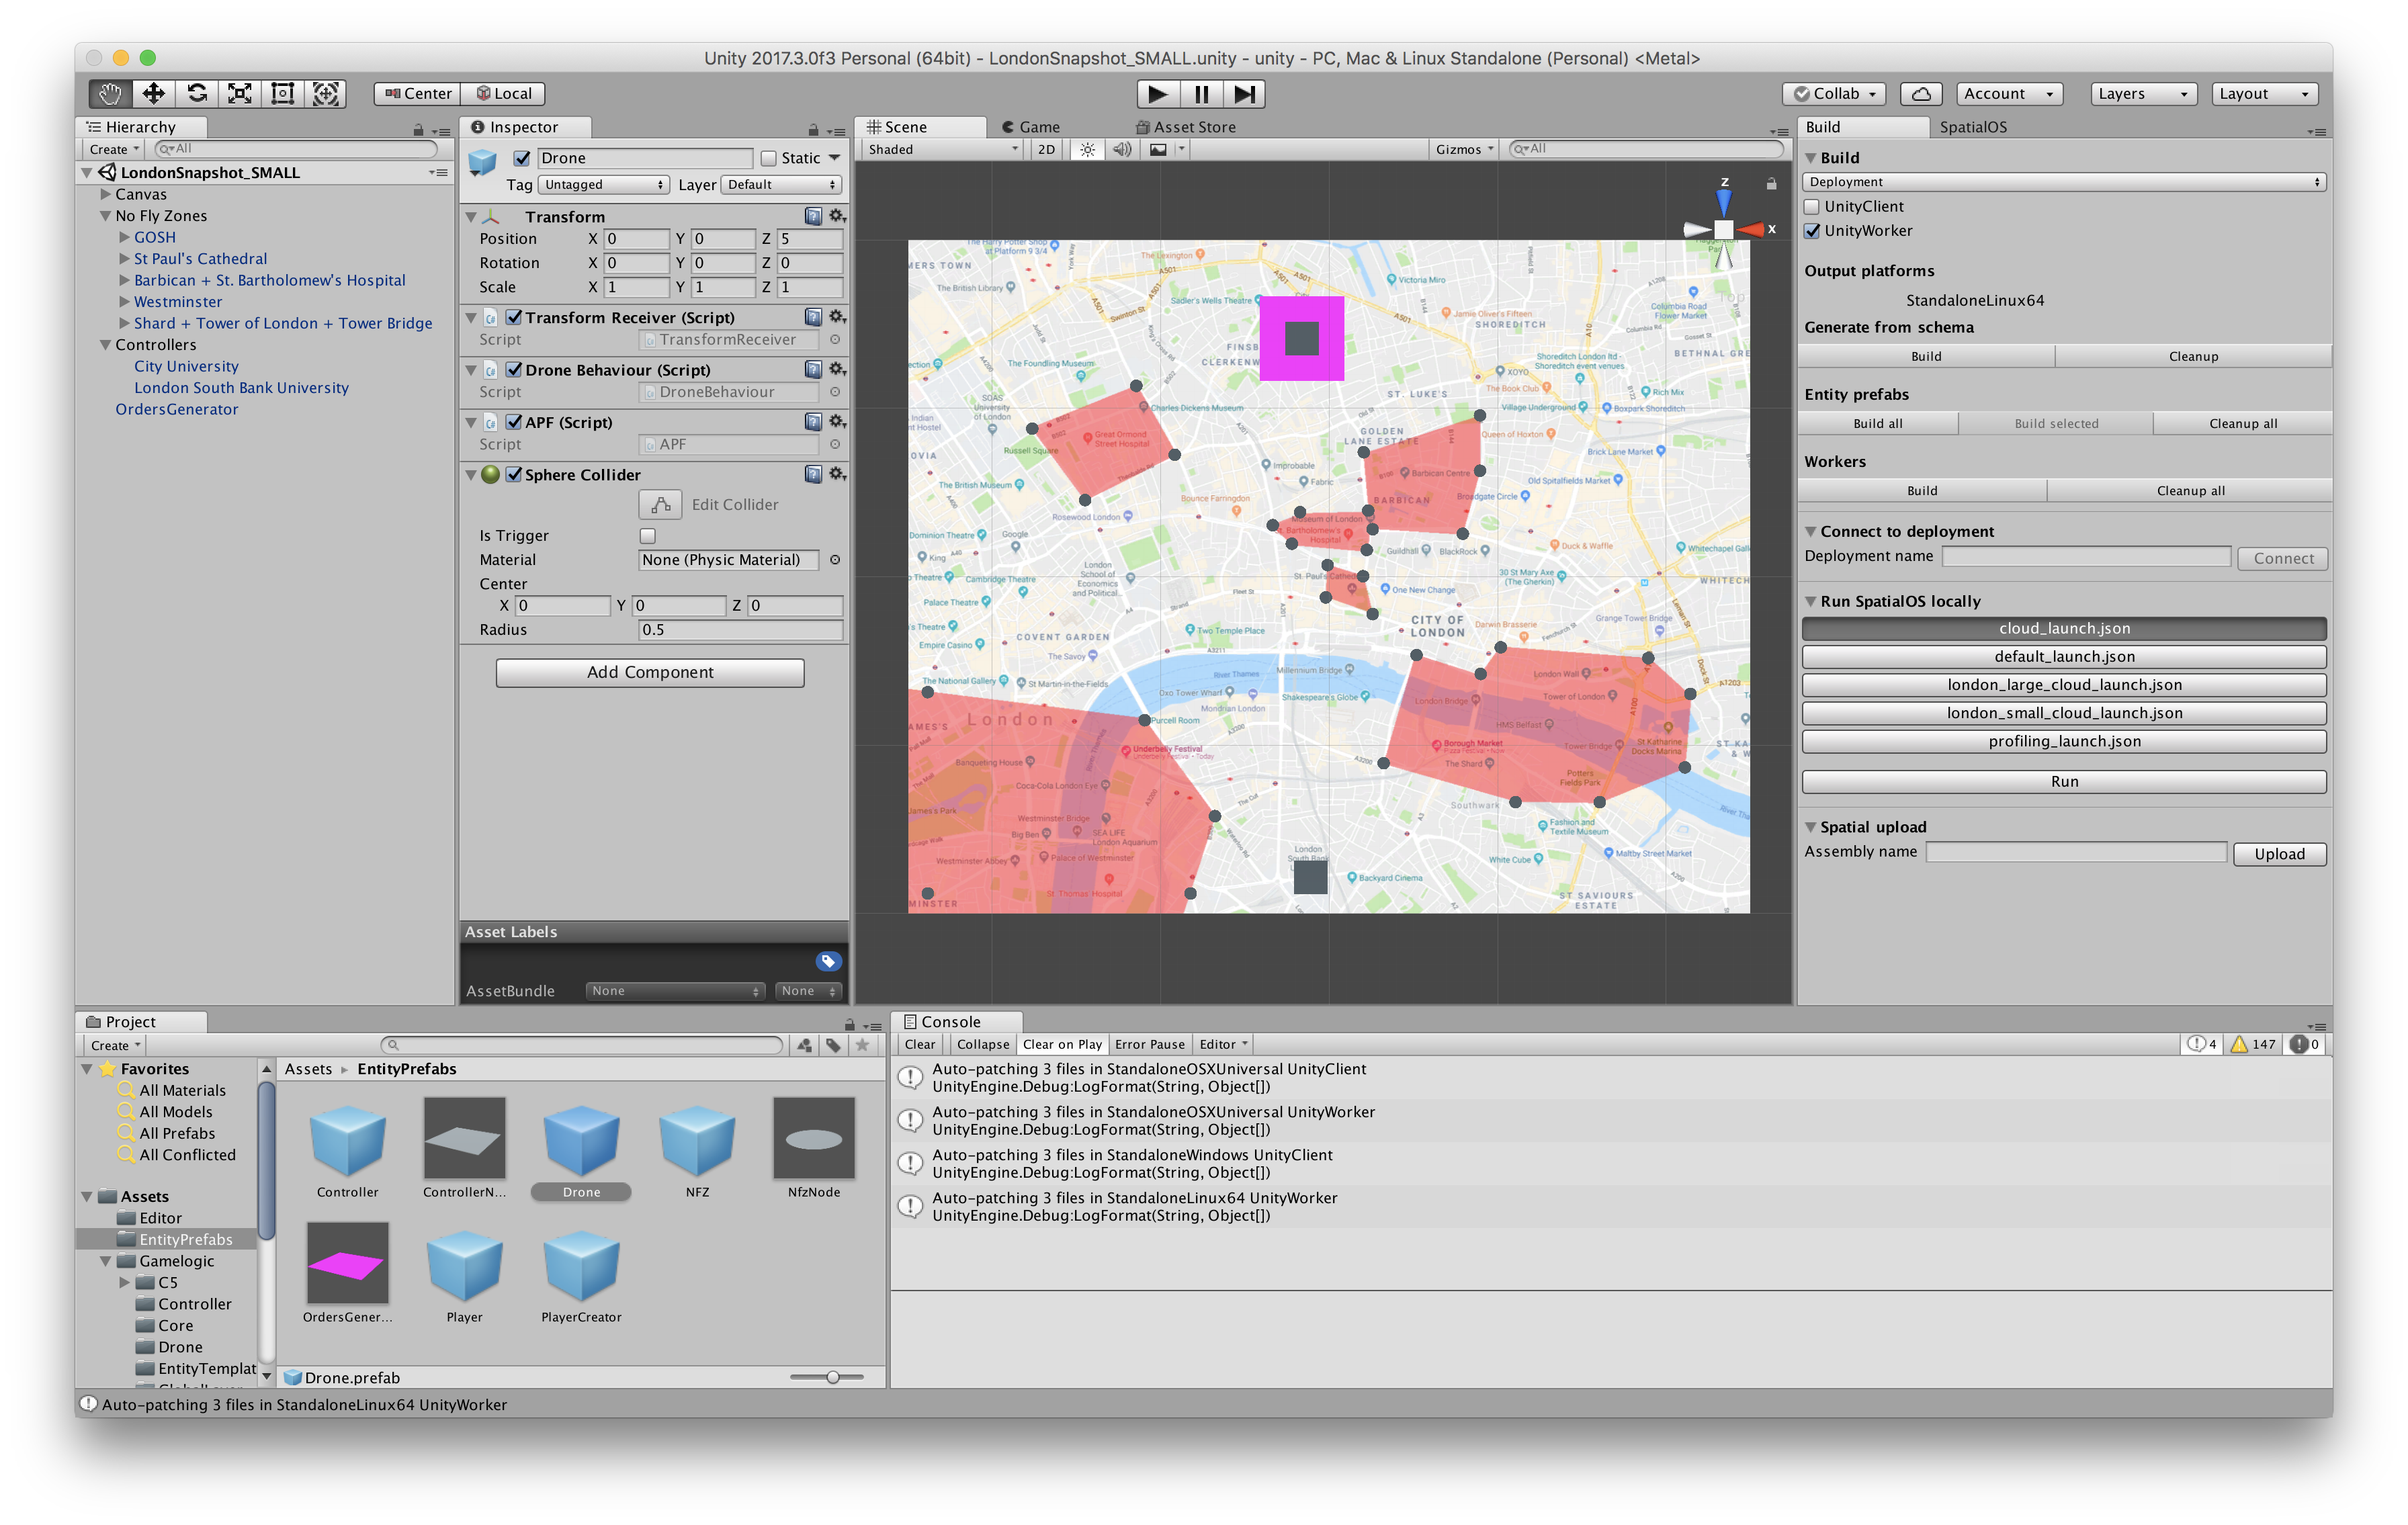
\includegraphics[width=\linewidth]{img/unity_londonsnapshotsmallexample.png}
  \caption{Viewing the London scene in the Unity Editor.}
  \label{fig:unity_londonsnapshotsmallexample}
\end{figure}

The world view in the middle is for visual aid when placing entities in the scene, with red highlights indicating parts of the world that are No Fly Zones. The column on the far right is a menu for SpatialOS build operations. This menu is particularly useful as being able to quickly rebuild the project within the Unity Editor greatly reduces iteration times.

\subsection{Representing No Fly Zones}
Earlier we defined No Fly Zones as a list of vectors to represent its vertices. To accurately place them in a scene, we create the \textit{NFZ} and \textit{NfzNode} prefabs in addition to a complementary \textit{NFZScript} MonoBehaviour.\\

\begin{sexylisting}[colback=white]{NFZScript MonoBehaviour}
using Improbable;
using Improbable.Controller;
using UnityEngine;
using System.Collections;

public class NFZScript : MonoBehaviour
{
  public GameObject[] nfzNodes;
  public Improbable.Controller.NoFlyZone GetNoFlyZone()
  {
    List<Vector3f> positions = new List<Vector3f>();
    for (int i = 0; i < nfzNodes.Length; i++)
    {
      positions.Add(nfzNodes[i].transform.position.ToSpatialVector3f());
    }
    return NFZ_Templates.CreateCustomNoFlyZone(positions);
  }
}
\end{sexylisting}

The script exposes an array of GameObjects, which can then be populated via the Unity Editor. By placing NfzNode objects in the scene and then populating the script's objects with these, we hold information about each zone's vertices. During snapshot generation we simply iterate through these NfzNodes and extract their positional information to create a NoFlyZone struct.

\clearpage
Figure \ref{fig:nfz_representation_example} shows an instance of a NoFlyZone prefab being populated with NfzNodes around Great Ormond Street Hospital. Note that renaming an object for our clarity does not change its underlying prefab, making this a really effective workflow for rapidly adding No Fly Zones to a world.

\begin{figure}[!hbpt]
  \center
  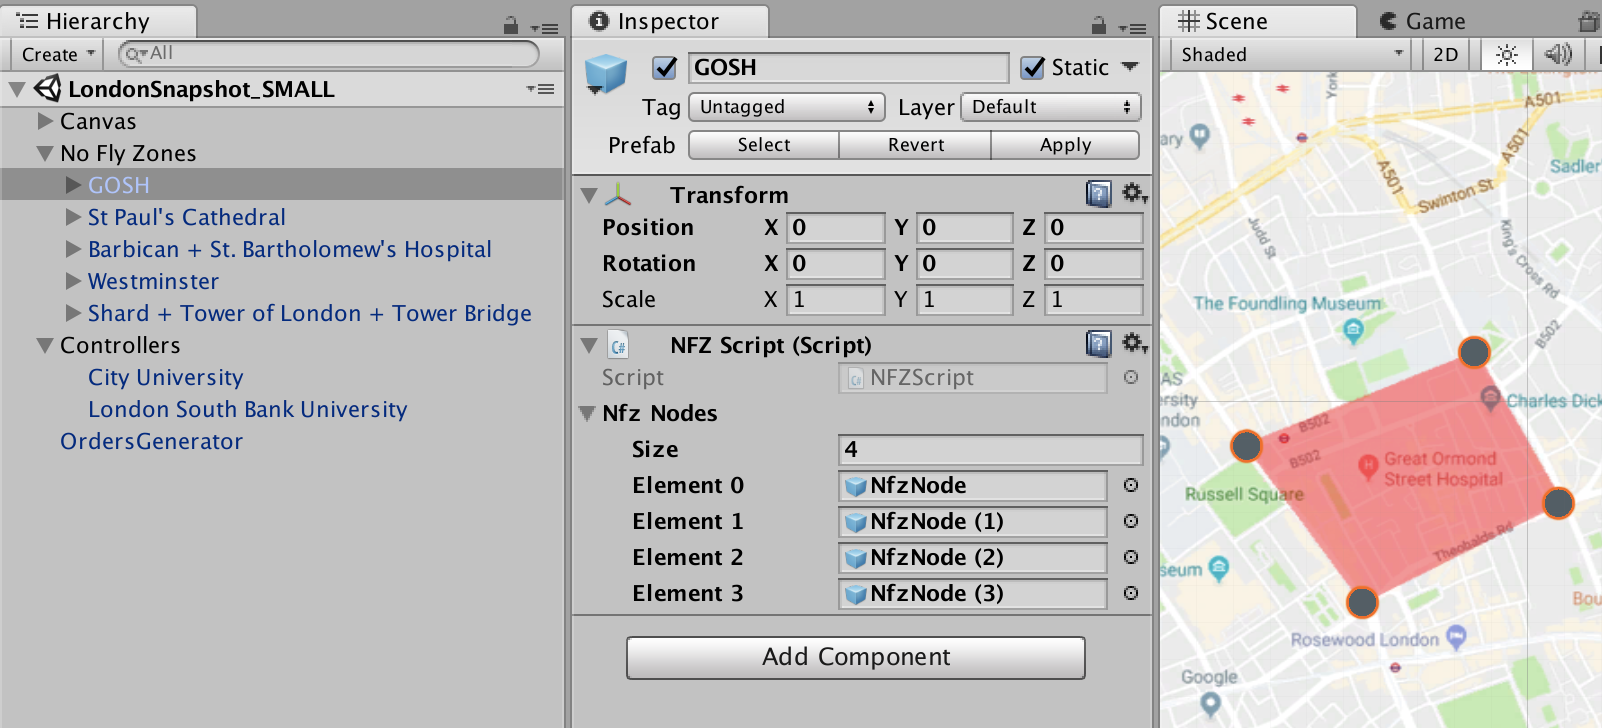
\includegraphics[width=0.85\linewidth]{img/nfz_representation_example.png}
  \caption{Inspecting GOSH's No Fly Zone.}
  \label{fig:nfz_representation_example}
\end{figure}

\begin{figure}[!hbpt]
  \center
  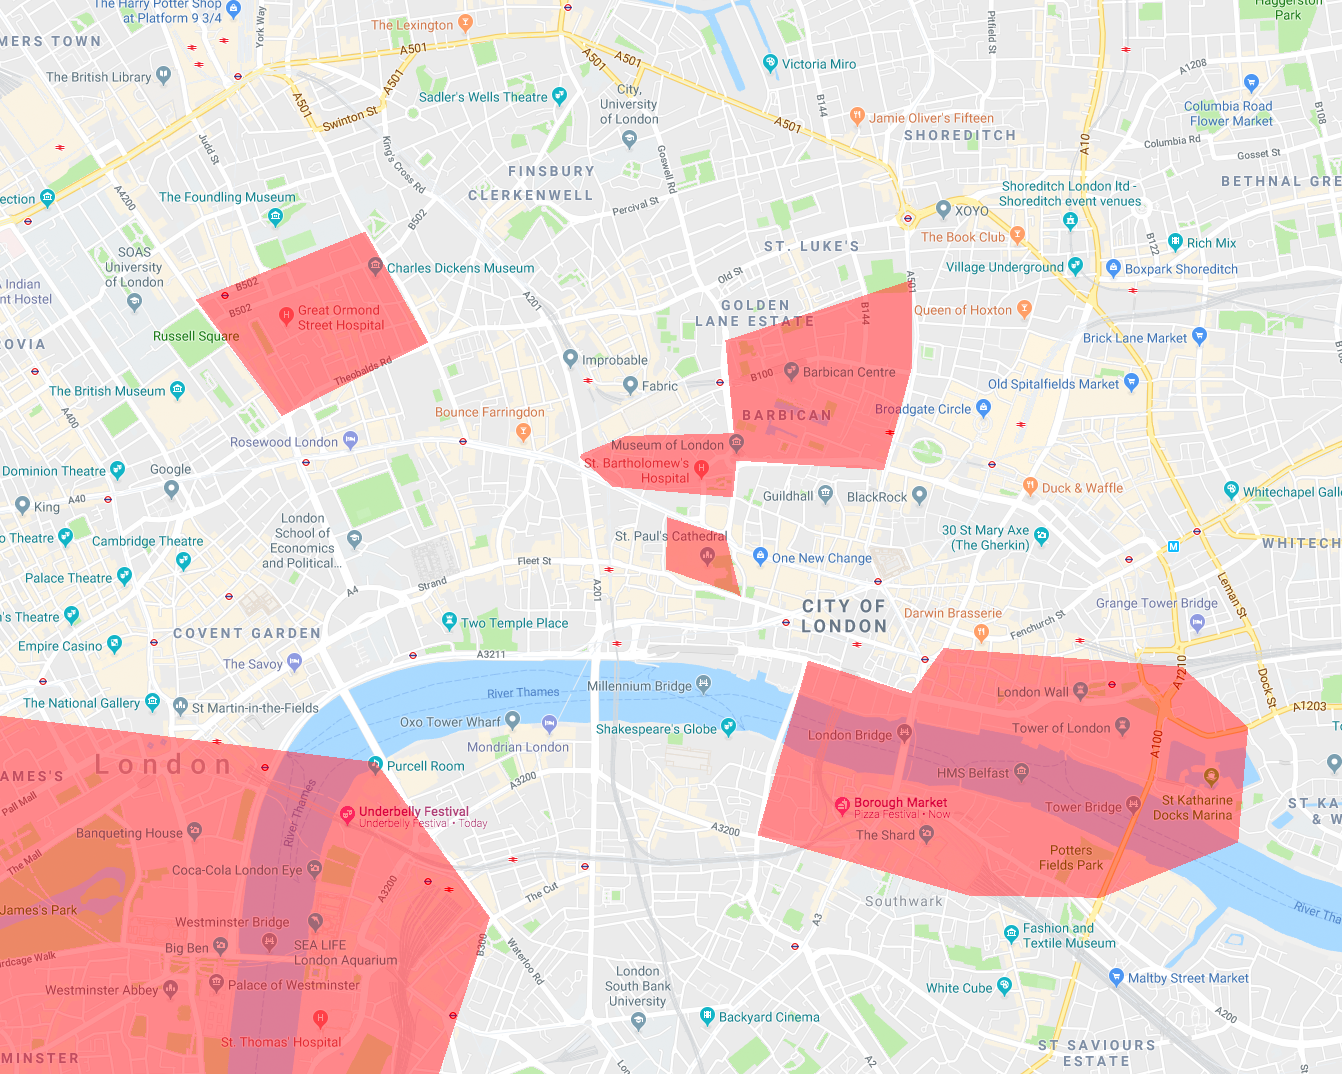
\includegraphics[width=0.85\linewidth]{img/london_snapshot_small_nfzs.png}
  \caption{Updated version of Figure \ref{fig:london_snapshot_small} with highlighted No Fly Zones.}
  \label{fig:london_snapshot_small_nfzs}
\end{figure}

\clearpage
\section{Entity Placement}
\subsection{No Fly Zones}
Making use of this new workflow, we added five major No Fly Zones to the world. Our intentions were to protect famous landmarks, public hospitals that may provide Air Ambulance support, the royal parks \cite{Blunden2016}, vertically large constructions and national security hotspots. To this end we placed No Fly Zones over:
\begin{enumerate}
   \item Famous Landmarks
   \begin{multicols}{2}
     \begin{itemize}
       \item Tower of London
       \item Tower Bridge
       \item St. Paul's Cathedral
       \item Westminster Abbey
       \item London Bridge
       \item Barbican
     \end{itemize}
   \end{multicols}
   \item Major Hospitals
   \begin{multicols}{2}
     \begin{itemize}
       \item St. Bartholomew's Hospital
       \item St. Thomas' Hospital
       \item Great Ormond Street Hospital
     \end{itemize}
   \end{multicols}
   \item Royal Parks
   \begin{multicols}{2}
     \begin{itemize}
       \item St. James' Park
       \item Hyde Park
     \end{itemize}
   \end{multicols}
   \item Tall Constructions
   \begin{multicols}{2}
     \begin{itemize}
       \item The Shard
       \item London Eye
     \end{itemize}
   \end{multicols}
   \item National Security Interests
   \begin{multicols}{2}
     \begin{itemize}
       \item Buckingham Palace
       \item Houses of Parliament
       \item Downing Street
     \end{itemize}
   \end{multicols}
\end{enumerate}

\clearpage
\subsection{Controller}
For a simulation of only 5km x 4km, we felt that there was no need for more than two controllers as we operated under the assumption that the simulation is only of an early-stage pilot delivery network. We scouted for two higher education establishments to act as Controller locations, coming up with a shortlist of University College London (UCL), SOAS University of London (SOAS), King's College London, London School of Economics (LSE), City University, and London South Bank University.\\

Not only do we have to consider the merits of each location, but how pairs of locations would work. For example, it makes little sense to have a ``distributed'' delivery network with two controllers in close proximity to each other. For this reason, we felt strongly that there should be one location below the river and one above, meaning that London South Bank University became the site of our first Controller.\\

After fixing one location, the flaws of others became more apparent. King's was rejected on the grounds that it was placed in an awkward position such that it would end up being responsible for far more of the map than South Bank would. LSE was in a prime position in the centre-left of the map, but with the location came the consideration that nearby hotels and fine dining establishments would not appreciate a major drone operation occuring above their property.\\

Lastly, UCL and SOAS were rejected for being too close to a major hospital zone. This left City University to become the host of our second Controller, giving us a nice bit of symmetry to the world layout.

\subsection{Order Generator}
Although its location does not have any bearing on the simulation outcome, the SpatialOS load balancer prefers to have this entity in the same place as any random Controller, so we stuck to our above-river bias and planted it under City University.

\subsection{Drones}
No drones exist in the world at startup because it is the job of a Controller to manage the life cycle of a drone. Therefore they do not need to be considered here.

\section{Snapshot Generator}
The actual process of collating all the objects in a scene and creating a snapshot file is triggered by the custom \textit{Drone Sim > Generate London Snapshot} menu option, shown below in Figure \ref{fig:menuotions}.

\begin{figure}[!hbpt]
  \center
  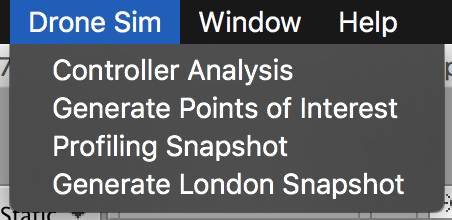
\includegraphics[width=0.5\linewidth]{img/menuotions.png}
  \caption{Custom drop-down options.}
  \label{fig:menuotions}
\end{figure}

This button then triggers a function to construct a snapshot, entity by entity:
\begin{enumerate}
  \item Reserve EntityId for Order Generator
  \item Initialise a Dictionary mapping EntityId to entity template
  \item Find NFZScript objects and extract each NoFlyZone
  \item Find Controller objects, pass in NFZ data, create template, store EntityId and position in a list, then add to dictionary
  \item Find OrderGenerator object, create template with NFZ data and controller details, then add to dictionary
  \item Use a given function to save out the dictionary as a binary snapshot file
\end{enumerate}

On successful creation, a log entry appears in the Unity Editor to say that a snapshot has been created at a particular filepath. This path is then used to point to a snapshot when launching local and cloud deployments.

\section{Custom Load Balancing}
Part of the reason so much thought has been put into Controller placement is the load balancer. Left to its own devices, SpatialOS moves its workers geographically around the simulation to best distribute load across workers.\\

Although this is brilliant for many use cases, our delivery network is operating under the assumption that each Controller is responsible for its own region with no real inter-region communication at this present point in time. Therefore, it makes sense to put each Controller onto a worker of its own, and minimise as best as possible the overlaps between each region and worker.\\

To do this, we update the worker launch configuration to make use of \textit{Point of Interest} load balancing \cite{ImprobableWorldsLtd.2018d}. This strategy works by specifying key locations that must not be simulated by more than one worker in the world, trusting the load balancer to divide and distribute regions of the world across a specified number of controllers. Each region consists of an area of the world closest to a given point of interest, like a Voronoi diagram.

\begin{figure}[!hbpt]
  \center
  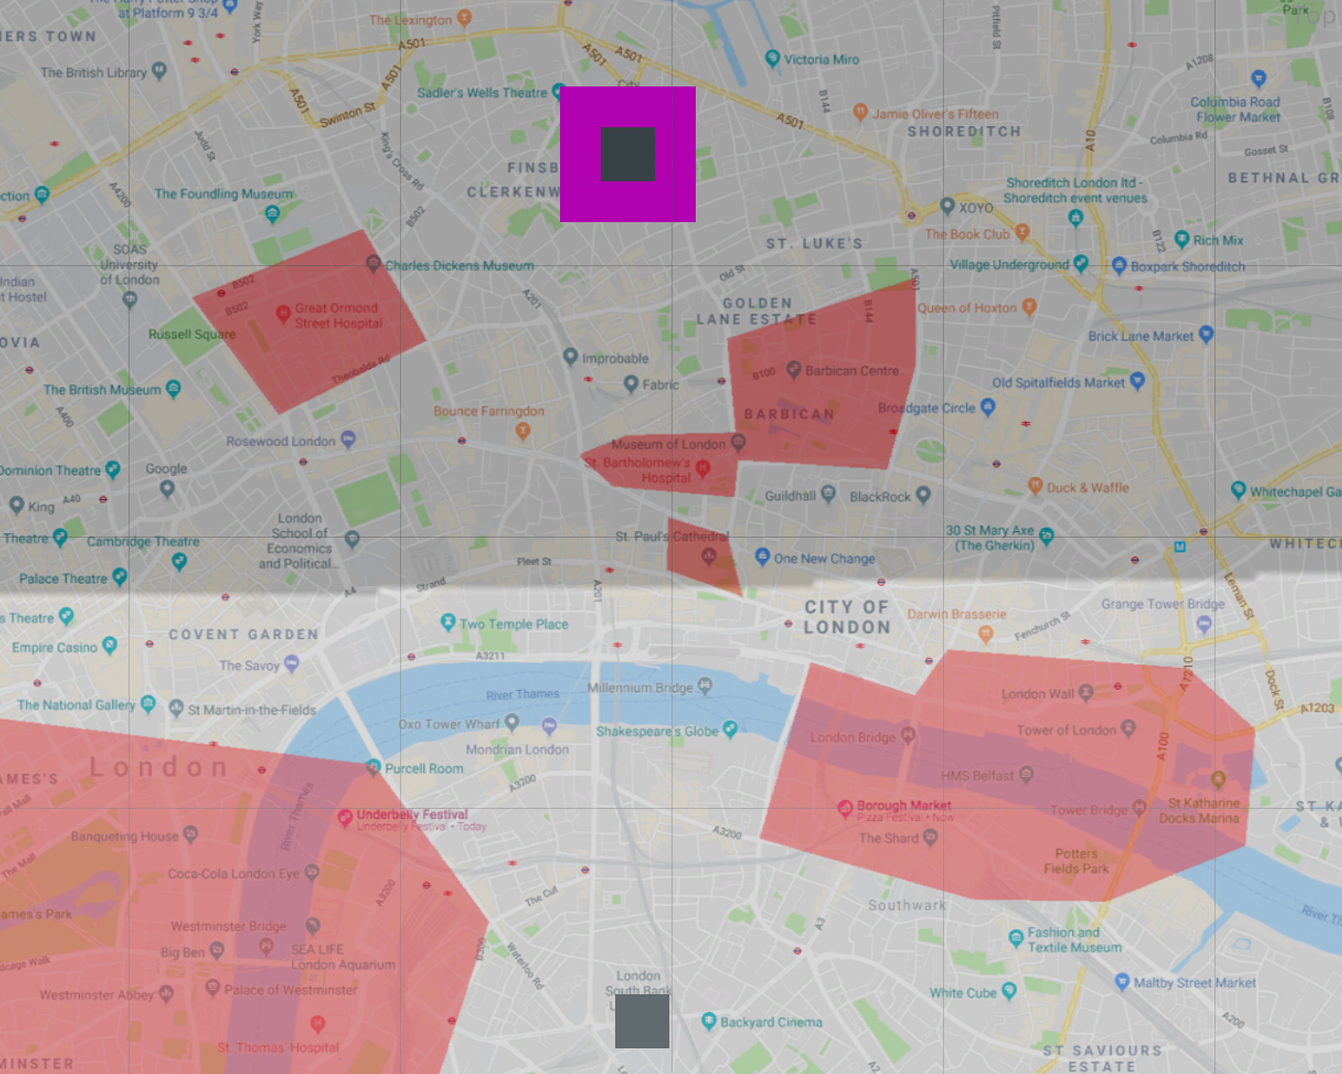
\includegraphics[width=0.8\linewidth]{img/smol.png}
  \caption{Voronoi diagram of the London snapshot.}
  \label{fig:smol}
\end{figure}

\clearpage
To generate our own Voronoi diagram of the world, we assign each controller a colour, traverse our world's map and assign a colour to each point based on which controller was closer. After looping through the map, we are given a nice visual representation of the area split. One observes in Figure \ref{fig:smol} that the two shaded regions of the world are fairly even in size, a positive sign that delivery requests are likely to be balanced well between controllers.

\begin{figure}[!hbpt]
  \center
  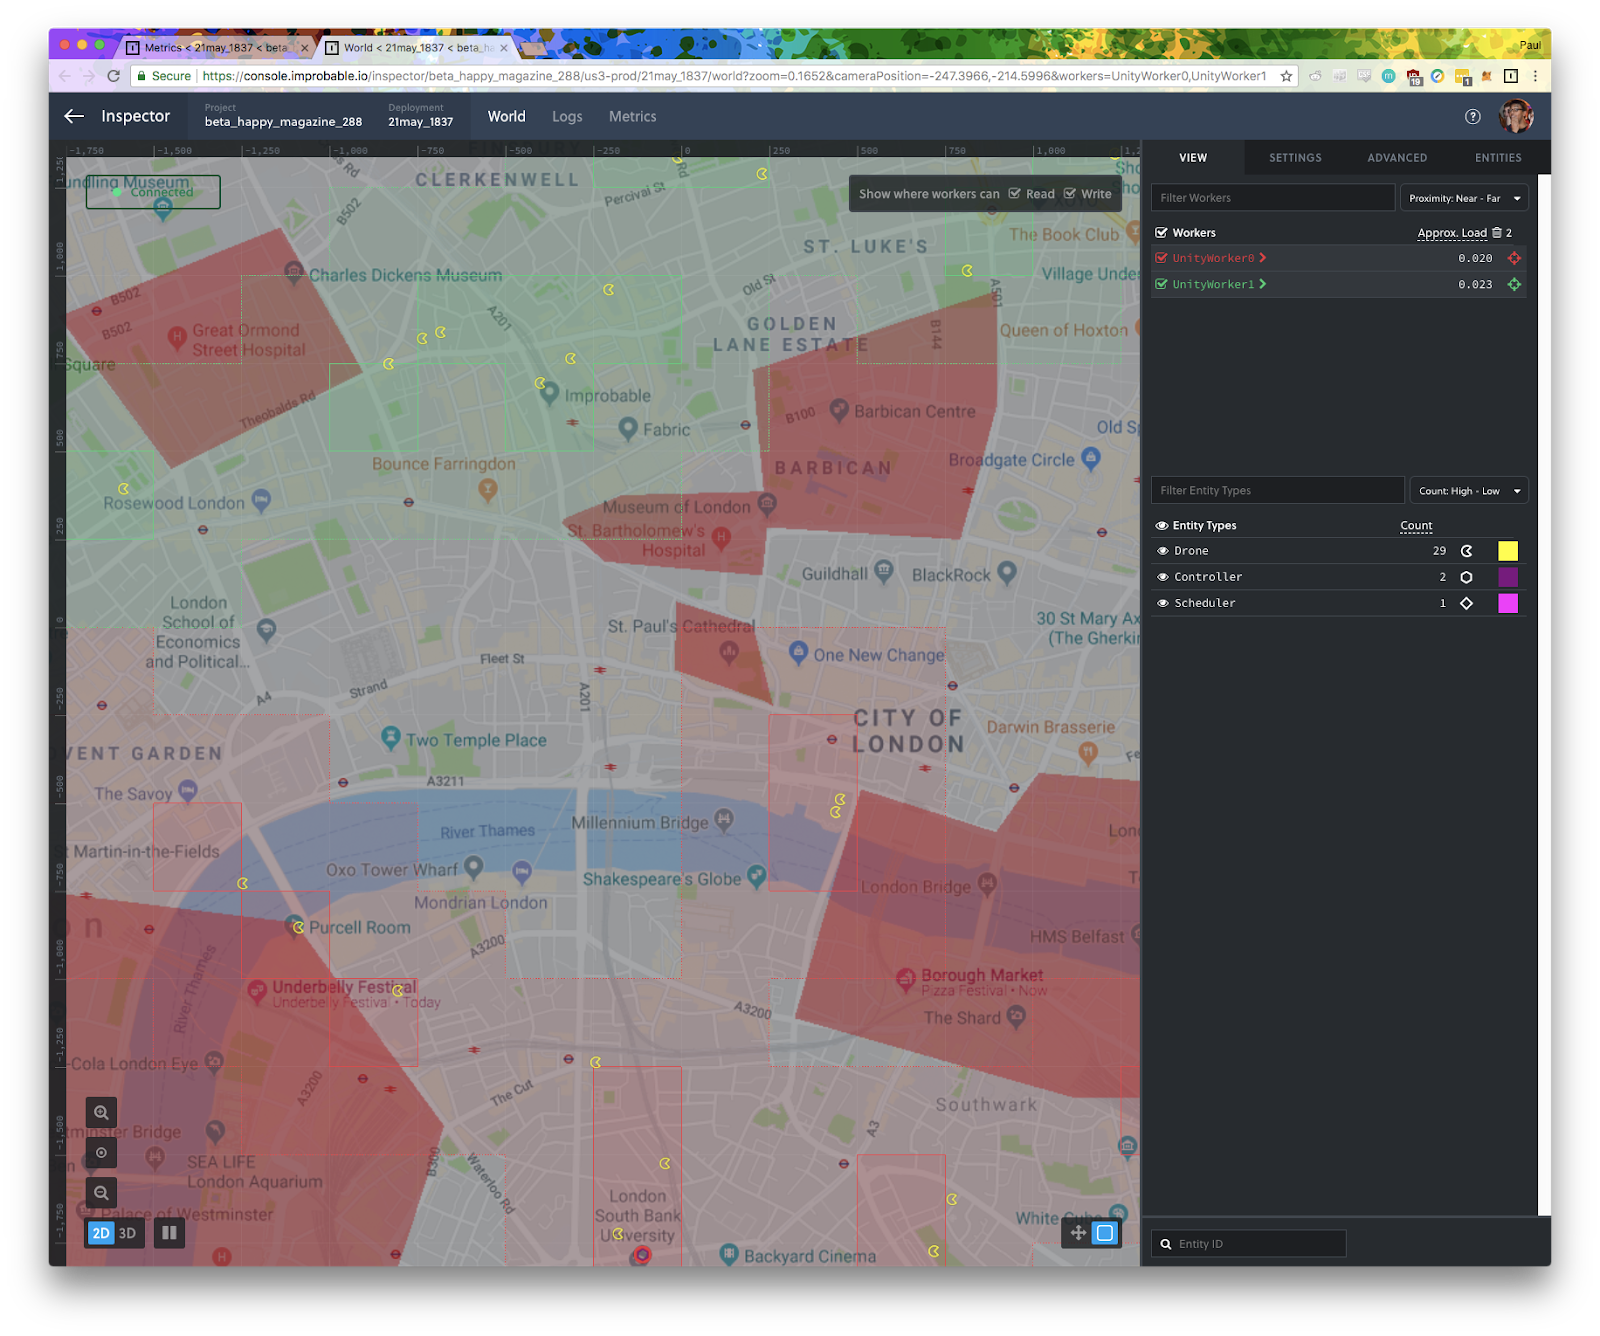
\includegraphics[width=0.95\linewidth]{img/gdoc2.png}
  \caption{SpatialOS view of a running simulation. Note that \textit{OrderGenerator} has been incorrectly labelled as \textit{Scheduler} in the image.}
  \label{fig:gdoc2}
\end{figure}

When inspecting a live simulation through the SpatialOS Inspector such as in Figure \ref{fig:gdoc2}, one can clearly see the worker boundary split the world through the middle. Though as mentioned before, SpatialOS constantly tweaks the load balancer so the boundaries may move around slightly as each region's load fluctuates with the ebb and flow of incoming orders and drone availability.

%**********************************************%
\newpage
\chapter{Integrating Delivery Economics}
With a basic London-scale simulation implemented to handle the logistical operations of a drone delivery network, we now look at how to extend this work to factor in, and later optimise for, the economic side.

\section{Improved Order Generation}
Before we can define a revenue model for our delivery network, we must improve the Order Generator to generate a greater variety of delivery requests. Packages being delivered by drones will vary in size, weight and priority, just like current the delivery market, and the DeliveryHandler schema needs to upgraded (Appendix A.4) to support these new properties of a delivery request.

\subsection{Package Type \& Weight}
We take our definitions of package types from Amazon's own \textit{Fulfilment by Amazon} service, as described by Figure \ref{fig:fulfilled_by_amazon_table} in Section 2.2. Subsequently we update the \textit{DeliveryRequest} schema type to include a new \textit{PackageInfo} property, to capture both the package type and weight. Each of the 6 package types accepts a different range of weights, hence generating a PackageInfo is (at the moment) a case of randomly picking a type, and then generating a random number within each type's accepted weight range.

\subsection{Delivery Priority}
In addition to the actual package information, each delivery request may have a priority corresponding to how urgently a customer wants their order to be delivered. Existing delivery companies each have their own range of services to customers, so to simplify this parameter we define four levels of priority: STANDARD, PRIORITY, URGENT and SUPER\_PRIORITY. We randomly select a priority for now, with the option to adjust bias further down the line just like with package types.

\section{Revenue Model}
As we are adopting the package types described by the \textit{Fulfilment by Amazon} programme, it makes sense to adopt their pricing model too as a starting point for standard priority deliveries.\\

Since we aim to provide a better service to orders with higher priorities, the price for each priority tier is a 50\% mark up from the previous tier. For example, standard delivery of a large letter would generate 80p, but priority delivery would generate £1.20 (80p x 1.5).\\

In addition to the priority system, we introduce a mechanism whereby the cost to a consumer per delivery, ergo ther revenue generated, decreases with the time taken to perform said delivery. The cost is halved if it takes more than 30 minutes to deliver the package after order generation, and reduced to 0 if the delivery takes more than 60 minutes to complete.\\

By charging both bigger fees for higher priority requests we provide incentives for controllers to prioritise more important requests to generate more revenue. However by offering reductions for slower delivery of goods, we also ensure that controllers attempt to serve all delivery requests as soon as possible.

\begin{table}[!hbpt]
\centering
\caption{Package Revenue Distribution.}
\label{fig:package_revenue_distribution}
\begin{tabular}{|c|c|c|c|c|c|}
\hline
\multirow{2}{*}{Package Type} & \multirow{2}{*}{Weight (g)} & \multicolumn{4}{c|}{Delivery Fee (£)} \\ \cline{3-6}
 &  & Standard & Priority & Urgent & Super Priority \\ \hline
\begin{tabular}[c]{@{}c@{}}Small\\ Letter\end{tabular} & 0 - 100 & 0.60 & 0.90 & 1.35 & 2.03 \\ \hline
\begin{tabular}[c]{@{}c@{}}Large\\ Letter\end{tabular} & 0 - 250 & 0.80 & 1.20 & 1.80 & 2.70 \\ \hline
\begin{tabular}[c]{@{}c@{}}Small\\ Envelope\end{tabular} & 0 - 100 & 1.09 & 1.64 & 2.45 & 3.68 \\ \hline
\multirow{3}{*}{\begin{tabular}[c]{@{}c@{}}Standard\\ Envelope\end{tabular}} & 0 - 100 & 1.21 & 1.82 & 2.72 & 4.08 \\ \cline{2-6}
 & 101 - 250 & 1.34 & 2.01 & 3.02 & 4.52 \\ \cline{2-6}
 & 251 - 500 & 1.54 & 2.31 & 3.47 & 5.20 \\ \hline
\begin{tabular}[c]{@{}c@{}}Large\\ Envelope\end{tabular} & 0 - 1000 & 1.77 & 2.66 & 3.98 & 5.97 \\ \hline
\multirow{6}{*}{Parcel} & 0 - 250 & 1.73 & 2.60 & 3.89 & 5.84 \\ \cline{2-6}
 & 251 - 500 & 1.79 & 2.69 & 4.03 & 6.04 \\ \cline{2-6}
 & 501 - 1000 & 1.84 & 2.76 & 4.14 & 6.21 \\ \cline{2-6}
 & 1001 - 1500 & 2.26 & 3.39 & 5.09 & 7.63 \\ \cline{2-6}
 & 1501 - 2000 & 2.48 & 3.72 & 5.58 & 8.37 \\ \cline{2-6}
 & 2001 - 3000 & 3.32 & 4.98 & 7.47 & 11.21 \\ \hline
\end{tabular}
\end{table}

\clearpage
\section{Operating Costs}
To calculate the profitability of the drone delivery network, we need to consider the costs of operating such a system. For our simulation we have identified the main sources of expenditure to be the energy consumption overhead of running the drones, along with any penalties that may be charged for failed deliveries and mid-flight collisions.\\

Although we have designed each Controller to act as a delivery dispatch point, like an Amazon Fulfilment Centre, we do not consider the costs of running such a warehouse. Instead we only focus on economic matters that are influenced by our newly introduced drone delivery dynamics.

\subsection{Energy Consumption}
As a baseline to model our simulated drones on, we look at information available about Amazon Prime Air prototypes. We can compute the expense of running the drones by first keeping track of a drone's energy usage per delivery, then multiplying it by the cost per unit of energy.\\

We know that the power rating of a moving drone is 8355.1W, but we must compute the power of a drone hovering ourselves using the current and voltage readings. Using a basic understanding of Physics, we define energy and power below.
$$energy = power * time$$
$$power = current * voltage$$

The prototype in question \cite{Jung2017} has 8 motors, each rated at 36.59V and 2.29A. Giving us a power rating of 670.3W when the drone is hovering.
$$ 8\ motors * 2.29A * 36.59V = 670.3W $$

Because we move drones at fixed time intervals, we can pre-calculate the energy increments depending per drone state. When updating the position of the drone every 0.25 seconds, we can also increment the energy usage by these fixed amounts. Being able to calculate these in advance reduces the work we have to do on every call to \textit{MoveDrone()}.

\clearpage
$$ energy\ (motion) = 8355.1 * DroneMoveInterval\ (seconds) = 2088.775\ Ws $$
$$ energy\ (hover) = 670.3 * DroneMoveInterval\ (seconds) = 167.575\ Ws $$

Once a drone completes its delivery and has returned to the Controller, we can compute the total cost of performing said delivery. Taking into account the different units of time used so far:
$$ cost\ of\ delivery\ (pence) = energy\ usage * 0.0055 / 3600 $$

We believe delivery network operators would be able to source electricity at wholesale rates, which we found to be around £55 per MWh \cite{Ambrose2018}, or 0.0055p per Wh.

\subsection{Penalties}
Understandably, nothing will ever work perfectly forever. To mitigate bugs in the simulation, we periodically ``prune'' drones that have been unresponsive for too long. We therefore consider the penalties applied for actions the drone has failed to complete at the time of pruning. We therefore define four main infractions:
\begin{multicols}{2}
  \begin{enumerate}
    \item Failed Launches
    \item Failed Deliveries
    \item Failed Returns
    \item Collisions
  \end{enumerate}
\end{multicols}

When a drone is unable to be launched, we consider that a delivery request was accepted but then unable to be completed. From a consumer point of view, they may have received a notification indicating that their delivery is on their way, only to be quickly told that their order has been cancelled because of some error in launching a drone. In this instance we do not charge the customer any delivery fees, instead giving them a fixed £5 compensation.\\

If a drone is launched but still fails to deliver a package for whatever reason, we compensate the consumer as before and also calculate the cost of sending a truck to manually retrieve the drone that was sent out. When a drone fails to return for some reason \textit{after} making a delivery there is no reason to compensate the customer, but we still have to calculate the cost of retrieving the drone.\\

When calculating the cost of retrieving a drone, we model our lorry on a standard UPS delivery truck with a mileage of 13.1 miles per gallon \cite{Lammert2009}. We consider fuel prices to be 125.1p per litre \cite{TheAA2018}, which translates to 568.7p per gallon.
$$ retrieval\ cost = 2 * (distance * 0.621371) * mileage * fuel\ cost $$

In the event of a collision, we add a £400 (\$500 \cite{Jung2017}) penalty for every drone involved in the collision, assuming the worst case where each drone would need to be completely replaced. In addition to this, we add appropriate penalties for failed deliveries and add a unified cost of retrieving all the drones.

\section{Case Study: Delivering a Milkshake}
To demonstrate how cost effective drone delivery is, we create a hypothetical case where a customer would like to order a milkshake at late night from the comfort of her room. The round trip of picking up, delivering the milkshake and then returning back to the Controller is approximately 4.33km.

\begin{figure}[!hbpt]
  \center
  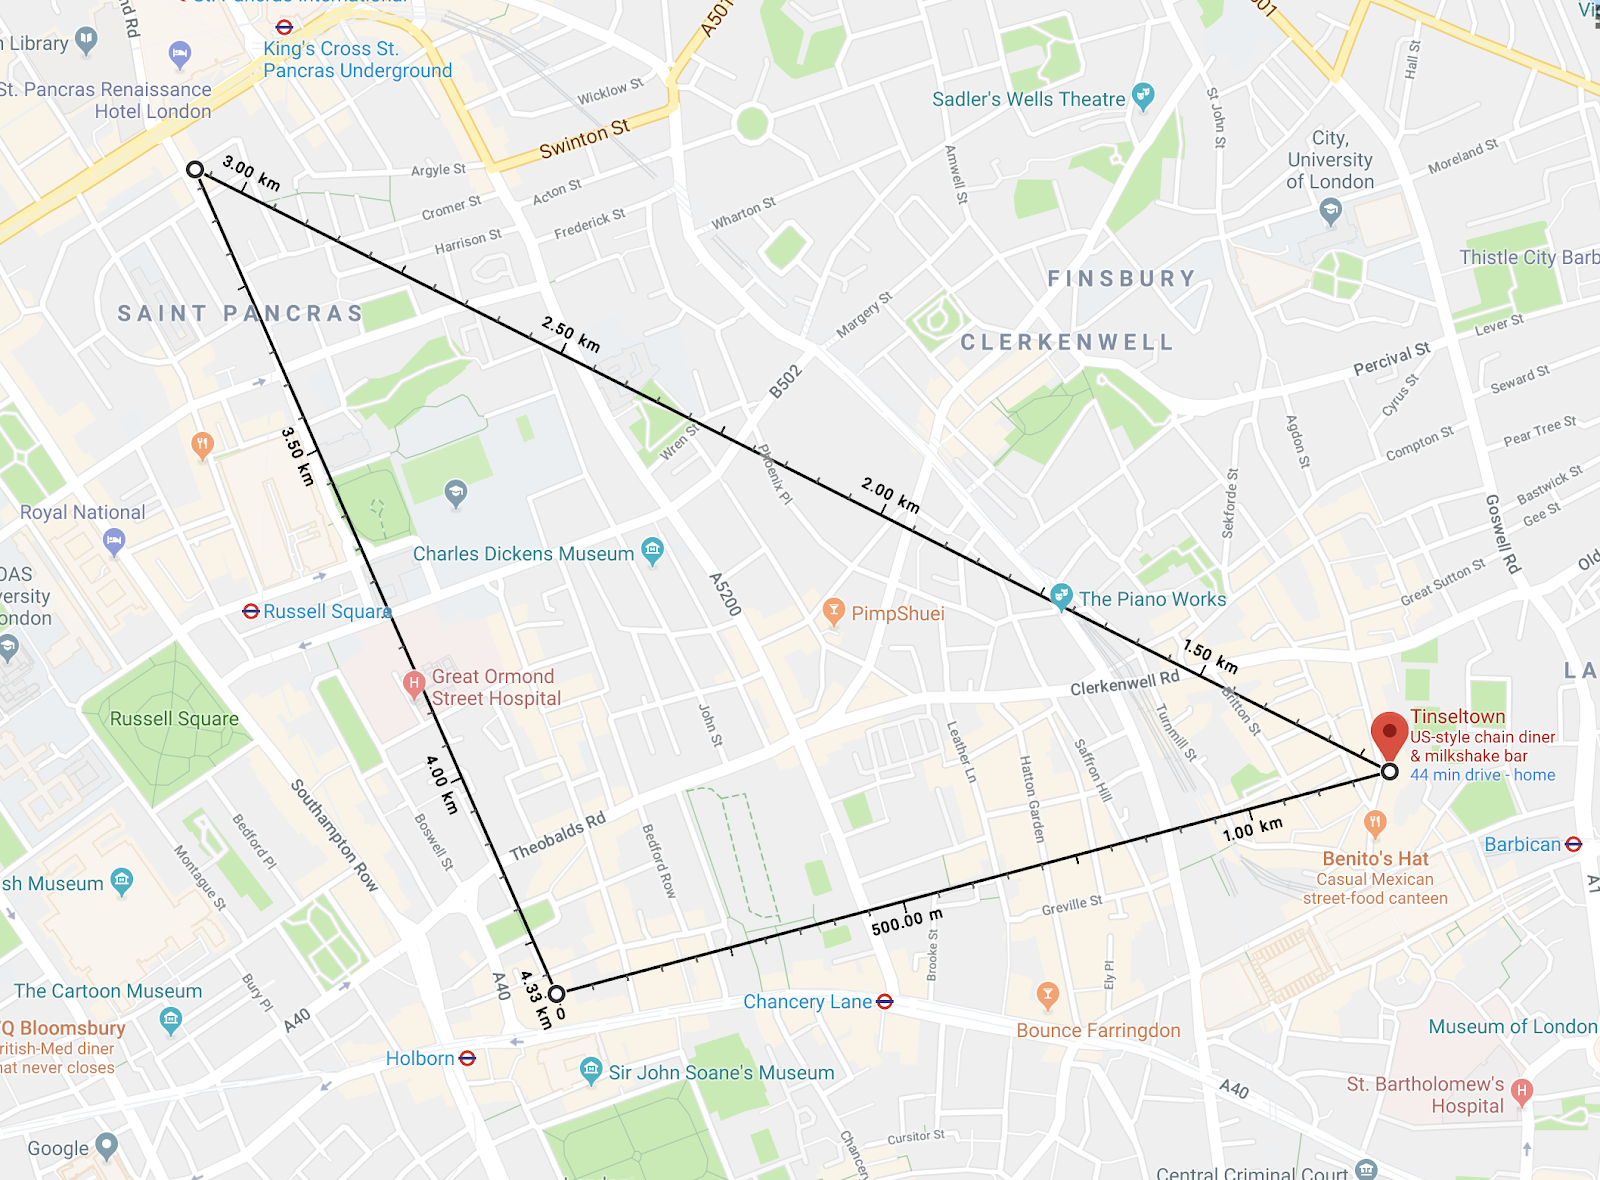
\includegraphics[width=0.9\linewidth]{img/drone_delivery_example_cost.png}
  \caption{Measuring the total distance of the delivery round trip.}
  \label{fig:drone_delivery_example_cost}
\end{figure}

For estimation sake, we assume that the drone is always moving. Therefore at a maximum speed of 10 metres per second, the drone would be in flight for 433 seconds. This corresponds to 3617758.3 Ws of energy use. Substituing this into our equation gives us:
$$ cost = 3617758.3 * 0.0055 / 3600 = 5.527130736\ pence $$

As per Table \ref{fig:package_revenue_distribution}, the revenue generated for standard delivery of an 800g milkshake is £1.84 for a operating costs of just 5.53p to the delivery network operator. As this is a mostly-autonomous system, the lion's share of generated revenue is pure profit.\\

For comparison, a large portion of Deliveroo's standard delivery fee £2.50 may be used to pay the delivery person. Perhaps the trickling down of these monetary, time and efficiency savings to the customer becomes the catalyst for increased drone adoption across delivery networks.

%**********************************************%
\newpage
\chapter{Time-Value of Delivery}
Before considering how to maximise profitability, we introduce the concept of the \textit{Time-Value of Deliveries} (TVD). This is based on the \textit{Time-Value of Data} idea we described earlier in Section 2.8. Rather than deal with the fixed pricing model of delivery fees as we see in the current day, we propose a new mechanism where the cost of the delivery is a function of the time taken to do said delivery. This is known as a Time-Value Function (TVF).\\

For example, a user may pay £5 for a delivery that takes less than 30 minutes but be charged nothing if it takes longer than one hour. One may recognise that we are already adopting an informal TVF that halves the delivery fee after 30 minutes, making it 0 if delivery takes over  1 hour. Note that ``delivery time'' is the time taken from a controller receiving an order to a drone reaching the requested destination.

\section{Function Representation}
To reduce the computational effort required to calculate the cost of a delivery, we simplify each TVF to have 10 steps at equal time intervals. By keeping an array of booleans, we simply toggle each step true or false to indicate whether there is a price drop at that step.\\

Figure \ref{fig:testpostplsignore} shows early concept art of a TVF with price drops at 18, 42 and 60 minutes. In this example, our array would have the the 3rd, 7th and 10th elements of the TVF array set to true.
$$ [0, 0, 1, 0, 0, 0, 1, 0, 0, 1] $$

For our model, we also state that the price decrease per step is constant per TVF. The maximum value of a delivery is therefore extracted from Table \ref{fig:package_revenue_distribution}. The value of a step decrease is the maximum value divided by the number of steps in the TVF. This is to reduce the transmission size of a TVF, as each delivery request may provide its own function.\\

An array of 10 booleans takes 10 bits, but an array of 10 integers for the value at each step would be 40 bytes, 32 times the number of bits. Considering a TVF will be sent with every delivery request and each controller maintains a queue of requests, reducing the memory footprint of a TVF may allow the simulation to scale better down the line.

\begin{figure}[!hbpt]
  \center
  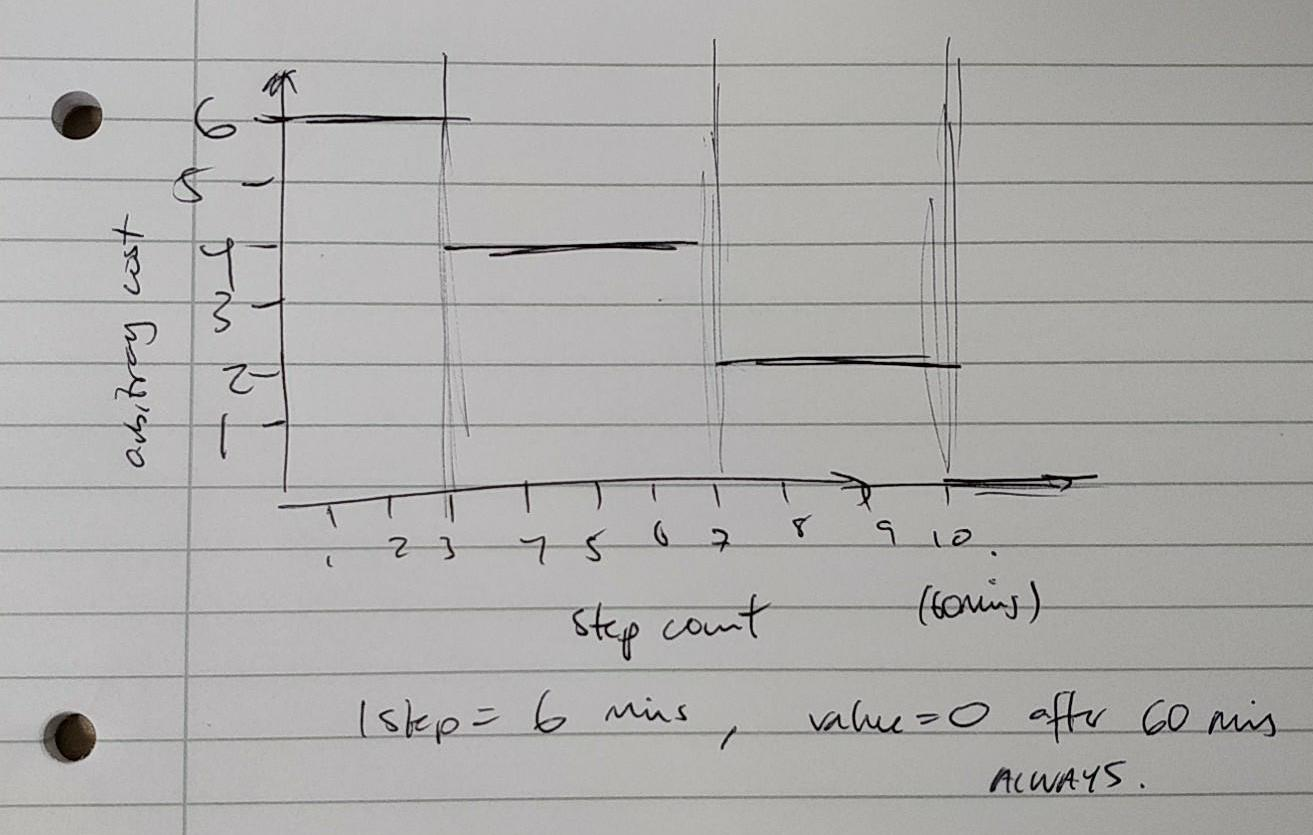
\includegraphics[width=\linewidth]{img/testpostplsignore.jpg}
  \caption{Conceptualising a Time-Value Function.}
  \label{fig:testpostplsignore}
\end{figure}

\section{Utilised Functions}
To integrate TVFs with our simulation, we update the Order Generator to support two models. For every delivery request generated, the Order Generator randomly chooses between \textit{The Halvening} or \textit{Stepwise Decrease} functions.

\clearpage
Although we could simply enumerate these two models and calculate the delivery fee using pre-defined value functions, our chosen implementation opens up the option to experiment with more complex TVFs in the future.

\subsection{The Halvening}
$$ [0, 0, 0, 0, 1, 0, 0, 0, 0, 1] $$

\textit{The Halvening} is a formalisation of the price-halving model we had already implemented before we introduced Time-Value Functions. By allowing longer periods of time before fee decreases, controllers are given more flexibility to, perhaps, schedule a higher priority request and still generate the same revenue on the other request. In general, this model might be best suited for a customer who is not \textit{too} strict on the swiftness of a delivery.

\begin{figure}[!hbpt]
  \center
  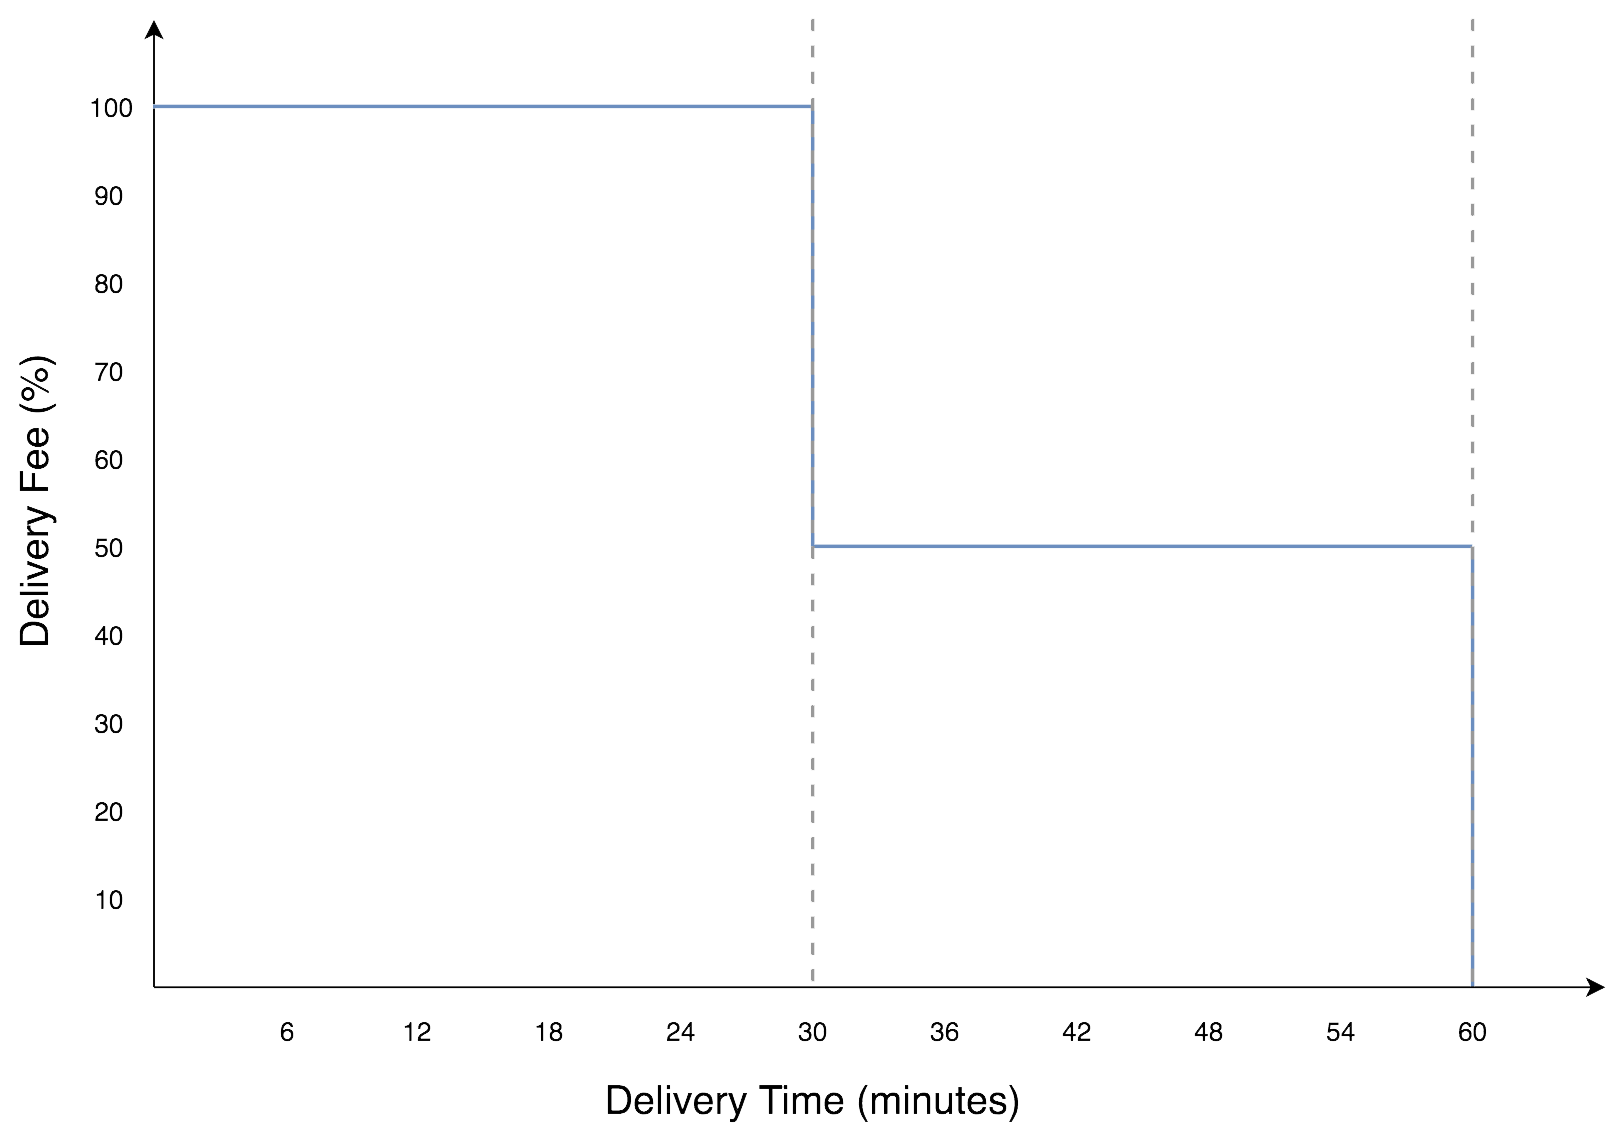
\includegraphics[width=\linewidth]{img/tvfs_halvening.png}
  \caption{Plotting \textit{The Halvening}.}
  \label{fig:tvfs_halvening}
\end{figure}

\clearpage
\subsection{Stepwise Decrease}
$$ [1, 1, 1, 1, 1, 1, 1, 1, 1, 1] $$

More customers may consider opting for this model as it enforces a fee decrease every 6 minutes, which means Controllers are given greater incentive to deliver orders with this TVF as quick as possible.

\begin{figure}[!hbpt]
  \center
  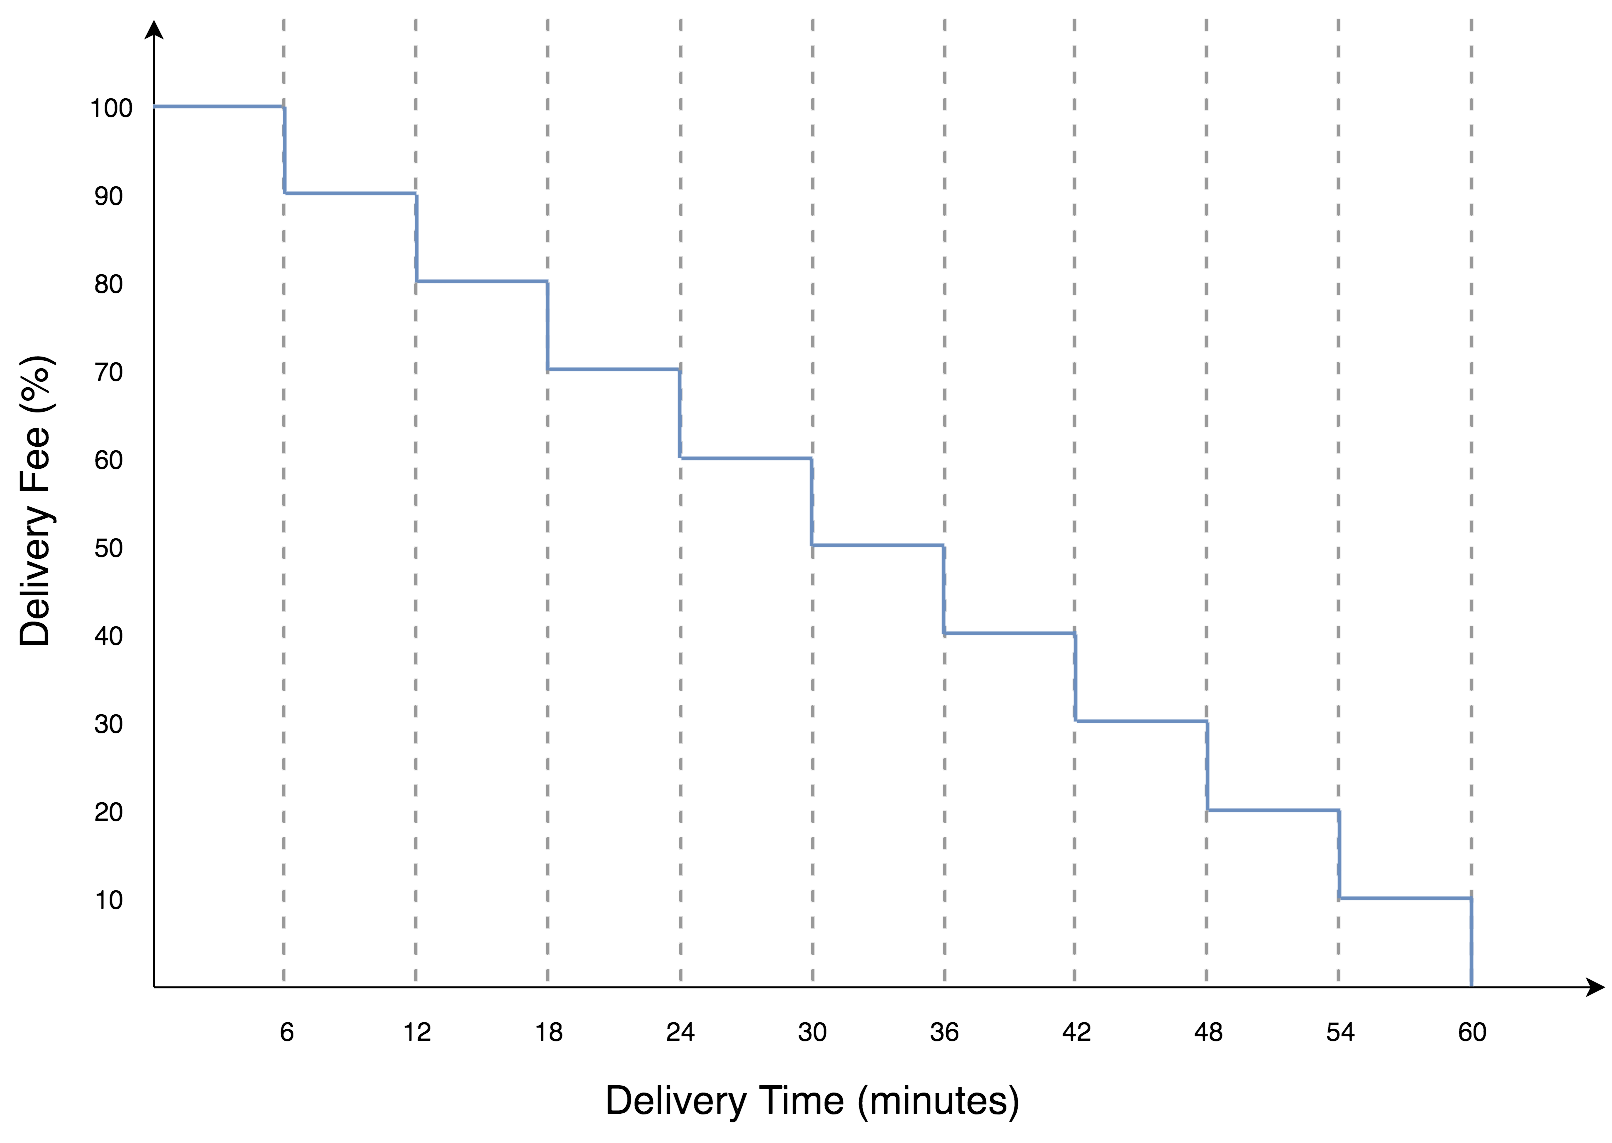
\includegraphics[width=\linewidth]{img/tvfs_decrease.png}
  \caption{Plotting \textit{Stepwise Decrease}.}
  \label{fig:tvfs_decrease}
\end{figure}

%**********************************************%
\newpage
\part{Optimisation \& Scale}
\chapter{Profit-Optimised Scheduling}
Our simulation now consists of a distributed delivery network, variation in order generation and a novel revenue model, but each Controller is still using a very primitive form of scheduling - First Come First Serve (FCFS). As we have demonstrated in Section 7.4, drone delivery networks are already extremely profitable, therefore in our simulation controllers do not stand to make any sort of loss. Nonetheless, there is no shadow of doubt that there are modifications that can be made to the scheduler to prioritise higher value orders and generate a greater profit.\\

In our simulation, each controller only operates 15 drones at a time with a maximum request queue size of 40. After this point orders will still be coming in, but a FCFS scheduler would simply discard any new requests to serve the existing queue. One would then imagine that by re-evaluating the request queue on each new order received to weed out lower value orders, we would be able to maintain requests with higher potential values and thus increase our profitability.\\

In order to make use of such a priority queue to filter out the lowest value orders, we must first define a way of assigning a priority to each request. For our simulations we have chosen to implement the novel \textit{Least Lost Value (LLV)} algorithm as our primary profit enhancing technique, as this approach takes advantage of the TVF-based revenue model.\\

In the interests of comparing LLV with a more popular but well-performing algorithm, we also take a look at and implement \textit{Shortest Job First (SJF)} scheduling.

\section{Least Lost Value}
As described earlier, the concept of deliveries having a value that decreases with the time taken to complete it is inspired by the \textit{Time-Value of Data (TVD)} model used in big data and business intelligence. Therefore when investigating methods of optimising our scheduler for profit, we looked at ways that big data jobs would be scheduled for optimal time-value of data.\\

Our quest for optimisations led to a meeting with a PhD student of our supervisor, Prof. Knottenbelt. The PhD student, Shireen Seakhoa-King, was working on a scheduling optimising tool for the Big Data use-case and was informed by our supervisor about the project described in this report. This opened the communication channels to discuss her tool and its potential applications further.\\

After multiple meetings it became clear that Shireen's tool was a TVD-based scheduling algorithm that claimed to process data with higher values compared to other TVD-based methods. Intrigued by this pitch, we agreed to implement her algorithm as our primary profit-optimising scheduling policy.

\subsection{Algorithm Overview}
As the name suggests, this algorithm aims to schedule items according to the \textit{Net Lost Value} metric. The next request to be taken from the queue is always the element with the lowest net lost value. To compute this value, LLV considers both the \textit{Potential Gain Value (PGV)} for performing a request as well the \textit{Potential Loss Value (PLV)} by doing other jobs later.\\

To calculate the \textit{Expected Value (EV)} of a job, its duration is modelled as a task duration distrubution in order to account for variance in execution times. This duration is then used to compute EV in a similar manner to what we have previously described with Time-Value Functions.
$$ EV(j_{i}, t_{c}) = \int_{t_{0}}^{\infty} V_{i}(t).f_{i}(t-t_{c})\ dt $$

\clearpage
The Potential Gain Value is therefore defined as the difference of value between processing a job now versus at a later time.
$$ PLV(j_{i}) = \sum_{j_{k}\in J,\ k\neq i,\ k-1}^{n} (EV(j_{k},t_{c}) - EV(j_{k}, t_{c}+p)) $$

The Potential Loss Value is defined as the sum of the lost value of all the other jobs that have not been selected.
$$ PGV(j_{i}) = EV(j_{k},t_{c}) - EV(j_{k}, t_{c}+\bar{p_{i}}) $$

Once these have been computed, the Net Lost Value per delivery is defined as Potential Gain subtracted from the Potential Loss.
$$ NLV(j_{i}) = PLV(j_{i}) - PGV(j_{i}) $$

The NLV is then computed as above for all jobs wanting to be scheduled, and the next job to be scheduled is the one with the lowest NLV.

\section{Adapting LLV for Delivery Scheduling}
To adapt the LLV algorithm for our specific drone delivery use case, we must consider how to model the duration distribution and also how to evict elements from the request queue when it becomes full.

\subsection{Duration Distribution}
To simplify the problem and reduce the computation complexity of the scheduler, we opt out of modelling the expected duration as a distribution. Instead, we assume the drone maintains a constant speed from start to end, and simply treat the duration as a fixed value derived from the distance between the controller and the delivery destination.
$$ estimated\ duration = \frac{distance\ to\ destination}{maximum\ drone\ speed} $$

Although this means that we do not consider the variance of delivery times due to factors such as dynamic collision avoidance, deviations in start and return positions, and the time taken for the drone to reach cruising altitude, this method allows us to obtain a quick and dirty estimation that can be re-calculated with ease.\\

Being able to re-calculate this value with ease is of particular interest because the expected duration is something that the LLV algorithm attempts to compute several times during the course of its execution. However, since our way of calculating this variable generates the same result every time for a particular order, due to delivery destinations being fixed, we can add this field as a property to the \textit{QueueEntry} schema type.\\

Calculating the value once, storing it and then re-using it further reduces the complexity of the LLV algorithm in our particular use case.

\subsection{Queue Implementation}
If the priority of a queue under LLV policy is the NLV, then for every item in the queue we would have to traverse all other elements in the queue to calculate that item's priority. Assuming queue size $n$, we find that the time complexity of sorting a queue under this mode of scheduling is $O(n^{2})$.\\

As each element's priority depends on the values of all other elements, we have to re-sort the queue every time an element is added or removed. Since we are expecting a new order to arrive approximately every 30 seconds, we get a $O(n^{2})$ operation running at least twice a minute for the entire uptime of a Controller!\\

Although a Controller makes an attempt to dispatch a drone every 10 seconds, we only remove elements from the queue at 10 second intervals when there is no contention among the requests for access to drones. By that, we mean that the priority of requests only really comes into play once we have more pending requests than available drones.\\

We attempt to keep our Controllers busy to give our schedulers (quite literally) a run for their money, but even in this case the time between dequeueing of requests may well be in the minutes range as we wait for drones to return from the deliveries they make. Therefore, it makes sense to only re-sort the request queue when \textit{DeliveryHandler} is polled by \textit{ControllerBehaviour} for the next request to serve.

\clearpage
Even if the number of elements in the queue grows beyond the maximum limit we set, we prune the queue after re-sorting to make sure that only the top 40 highest priority elements remain.

\begin{figure}[!hbpt]
 \centering
 \begin{tikzpicture}[node distance = 20mm and 35mm]
 \node [box](og)                {Order Generator};
 \node [box,right=of og] (dh)   {Delivery Handler};
 \node [box,right=of dh] (cb)   {Controller Behaviour};
 \node [box,below=of dh] (rq)   {Request Queue};
 \draw [->] (og.east) to node[midway, above] {DeliveryRequest} (dh.west);
 \draw [->] ([yshift=3mm] cb.west) to node[midway, above] {Dequeue()} ([yshift=3mm] dh.east);
 \draw [->] ([yshift=-3mm] dh.east) to node[midway, below] {DeliveryRequest} ([yshift=-3mm] cb.west);
 \draw [->] ([xshift=-3mm] dh.south) to node[midway, left] {Add()} ([xshift=-3mm] rq.north);
 \draw [<->] ([xshift=3mm] rq.north) to node[midway, right] {SortAndPrune()} ([xshift=3mm] dh.south);
 % \draw [->] ([xshift=3mm] dh.south) to ([xshift=3mm] rq.north);
 \end{tikzpicture}
 \caption{Request Queue Interaction.}
 \label{fig:request_queue_interaction}
 \end{figure}

\subsection{Preliminary Results}
Preliminary runs using the LLV scheduler appeared to demonstrate far better performance than our existing First Come First Serve (FCFS) scheduler, in terms of both average profit per delivery and the overall profit generated over the course of the simulation.\\

This proved to be an interesting development that piqued our curiosity into investigating how our Least Lost Value policy stacks up against a Shortest Job First (SJF) approach, which Shireen expressed was the only other scheduler that would beat LLV under some conditions in her own testing. There was especially great interest to see how the two schedulers would fare in our specific use case of a drone delivery network.

\clearpage
\section{Shortest Job First}
In this algorithm, the request queue would be ordered by the estimated time to complete each delivery. For the sake of estimation and to be consistent with our assumptions in LLV scheduling, we assume a constant drone speed. Hence, we can efficiently order the queue by the total distance (as the crow flies) from the controller to the request destination.
$$ time = distance / speed $$
$$ job\ length \propto distance $$

\subsection{Pruning}
For the LLV scheduler, we re-sort the queue on every poll for a new \textit{DeliveryRequest}. On the other hand the priority of a \textit{QueueEntry} in SJF scheduling does not change once it has been calculated, therefore we can add and remove requests to the queue using built in priority queue functions with ease.\\

When a new delivery request comes in and the queue is smaller than the maximum allowed size, we calculate its priority and add it to the queue. If the queue is already full we compare the new request with the lowest priority item in the queue, and remove which of these two requests has the lower priority.

\subsection{Comparison to LLV}
We hypothesise that the SJF scheduler will perform exceedingly well when it comes to the sheer volume of deliveries it completes because it prioritises the shortest request all the time. Naturally, over the same duration of time, shorter jobs on average will mean more completed deliveries.\\

However if the average profit generated by these jobs is too low for the higher volume to compensate, the LLV scheduler will perform better. At this point, it is hard to predict a winner without conducting a through evaluation of simulation data.

\section{Advanced Scheduler Implementation}
We implement our advanced schedulers as priority queues with custom comparators.

\subsection{Priority Queue}
To allow us to prune low priority items in addition to dequeueing those with the highest priority, we need to make use of a data structure that efficiently keeps track of both maximum and minimum entries. To this end, we make use of the C\#-native \texttt{SortedSet<T>} class \cite{Microsoft2018} due to its capability to easily return the maximum and minimum entries, and in doing so making use of a comparator that we can define ourselves.\\

\subsection{Custom Comparator}
Our priority queue will be of type \texttt{SortedSet<QueueEntry>}. As QueueEntry is a struct generated from the type we define in the Schema, we have to define our own method of comparing two different \texttt{QueueEntry} items and determining which is greater or if they are the same. The method that forms this comparison is known as a comparator. To aid the comparator, we introduce a \texttt{priority} component of type float to \texttt{QueueEntry}. We use this to determine if an element is greater or lesser than another one.\\

% \begin{sexylisting}[colback=white]{Updated QueueEntry Type}
% type QueueEntry {
%   float timestamp = 1;
%   DeliveryRequest request = 2;
%   float priority = 3;
%   float expected_duration = 4;
% }
% \end{sexylisting}

% \clearpage
To check equality, we initially decided to check if two timestamps were equal. Despite it being a grave computer science sin to compare floating points, our rationale was that it would be almost impossible for two orders to arrive at a Controller at the same time. In fact, it would also be extremely unlikely that two orders arrived with a time delta smaller than floating point precision. However, we noticed on test simulations that the queue size would continually increase every minute until the worker finally crashed.\\

To remedy this we added an \texttt{id} field of type \texttt{int64}(long) to the \texttt{DeliveryRequest} schema. By ensuring that the Order Generator keeps incrementing the id of each outgoing request, we would never have two requests with the same id. Being an integer type, we are able to check equality of the request ids without having to worry about floating point precision errors as before.\\

% \begin{sexylisting}[colback=white]{Updated DeliveryRequest Type}
% type DeliveryRequest {
%   int64 id = 4;
%   improbable.Vector3f destination = 1;
%   PackageInfo package_info = 2;
%   TimeValueFunction time_value_function = 3;
% }
% \end{sexylisting}

Our custom comparator now checks for equality of \texttt{DeliveryRequest.id} and if inequal orders elements based on their \texttt{QueueEntry.priority}.\\

\begin{sexylisting}[colback=white]{Custom Comparator Implementation}
class CustomComparer : IComparer<QueueEntry>
{
  public int Compare(QueueEntry x, QueueEntry y)
  {
    if (x.request.id == y.request.id)
    {
      return 0;
    }
    if (x.priority > y.priority)
    {
      return 1;
    }
    return -1;
  }
}
\end{sexylisting}

%**********************************************%
\newpage
\chapter{Scale Testing}
In order to test the scalability of our current delivery network architecture, we need to try scaling up our simulation. This involves generating a larger snapshot with more Controllers, allocating bigger regions of the world to each Controller, as well as tweaking both the Simulation and SpatialOS configuration settings to support a simulation at the scale we desire.

\section{Expanding London}
Using our experience from building the smaller snapshot of London as a starting point, we define our key considerations for drone delivery network snapshot design to be:
\begin{itemize}
  \item Simulation Settings
  \begin{multicols}{2}
    \begin{itemize}
      \item World Size \& Location
      \item Max Queue Size
      \item Max Drone Count
      \item Order Generator Interval
    \end{itemize}
  \end{multicols}
  \item No Fly Zones
  \item Controllers
  \begin{multicols}{2}
    \begin{itemize}
      \item Controller Count
      \item Distribution
    \end{itemize}
  \end{multicols}
\end{itemize}

\clearpage
\subsection{Simulation Settings}
\subsubsection{World Size \& Location}
As our first snapshot was very focused on central London, we want our expanded snapshot to extend outwards in all directions and encompass more of suburban London. Simulating more of the city provides us a larger canvas and greater ability to tinker about with Controller placement. Perhaps Controllers in suburban locations are able to deal with larger areas as less orders may be requested in the outer areas?\\

With these thoughts in mind we define the four corners of our world to be Richmond, Wembley, Goodmayes and Bexleyheath, as shown by the area in Figure \ref{fig:london_snapshot_large}. These bounds were selected as it encompasses a large variation in London land mass. Not only would it allow us to have a good amount of realistic No Fly Zones, we could also get decent diversity in the size and shape of zones.

\begin{figure}[!hbpt]
  \center
  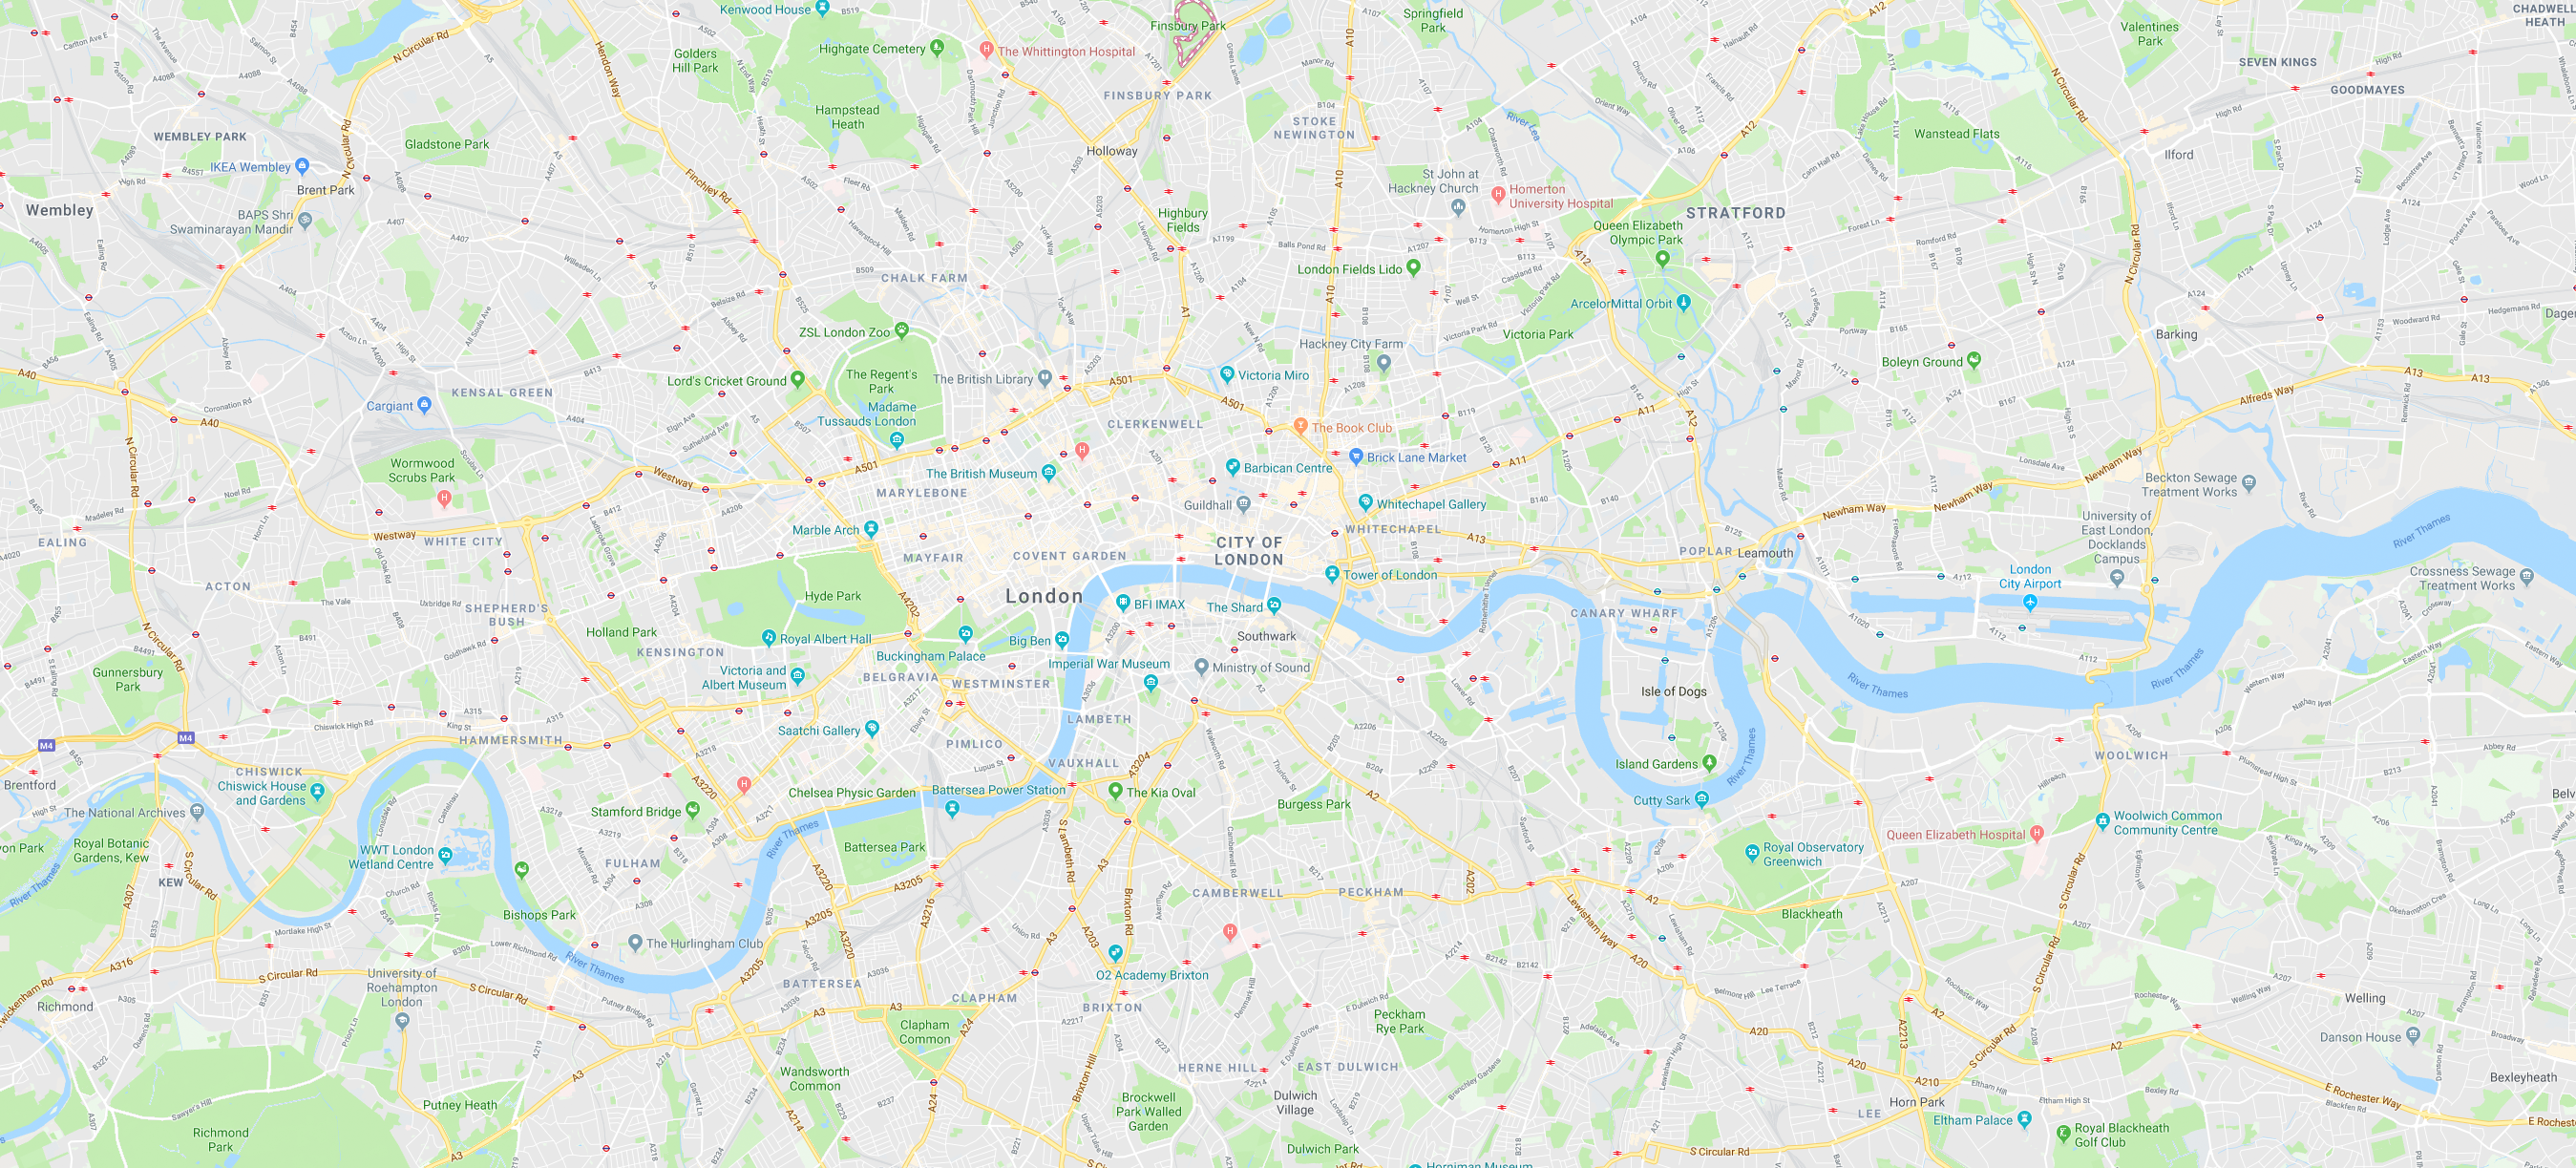
\includegraphics[width=\linewidth]{img/london_snapshot_large.png}
  \caption{Our large London snapshot.}
  \label{fig:london_snapshot_large}
\end{figure}

The new enlarged area we have chosen to simulate would generate a snapshot of London with dimensions of 32km x 14.5km, of which 31.5km x 14km is routable. For comparison our existing London snapshot has dimensions of 5km x 4km and a routable bounds of 4.8km x 3.8km, which means that the new snapshot represents over a 24x increase in routable area.

\subsubsection{Order Generator Interval}
Though the raw value of this variable is directly dependant on the number of Controllers we have to make use of in this world, we decide to double the expected incoming request rate per Controller so that we are able to observe how they deal with higher request volumes.\\

Suppose we deploy 20 Controllers, we would have to generate a new order every 1.5 seconds in order to average a new incoming \texttt{DeliveryRequest} every 30 seconds per Controller. In the new model doubling the rate means halving the interval time, meaning the OrderGenerator would now send out a new \texttt{DeliveryRequest} every 0.75 seconds.

\subsubsection{Other Settings}
As each Controller is expected to handle larger regions of land than before, we increase the number of drones per Controller from 15 to 20, and boost the maximum queue size from 40 to 50. If we doubled the request rate but also doubled the availability of all other resources, there is no net change in simulation behaviour except an increase in volume.\\

By scaling the various parameters differently, we aim to make life more difficult for the simulated delivery network. In this way, our scale test also can act as a stress test to pinpoint weakpoints in the system that need to be amended or mitigated before such a delivery network ``takes off'' in real life.

\subsection{No Fly Zones}
Though we lift the restrictions on adding No Fly Zones above major hospitals, we still maintain the rule regarding Royal Parks. Subsequently, we add 7 NFZs associated with Royal Parks to the snapshot. Until there is regulatory clarification over whether flying over parks could be a violation of several privacy rights, we also add Victoria Park, Olympic Park, Kew Gardens and Battersea Park to our list of parks protected by a No Fly Zone.\\

Note that the Regents Park NFZ is also the protector of both London Zoo and Lord's Cricket Ground.\\

As it is the financial and entrepreneurial hub of the capital, we protect the City of London under a No Fly Zone. London Bridge, Tower Bridge and the Tower of London can all be found under this NFZ. To avoid creating a massive blockade in the center of the city, we place the Barbican under a separate NFZ.

\begin{figure}[!hbpt]
  \center
  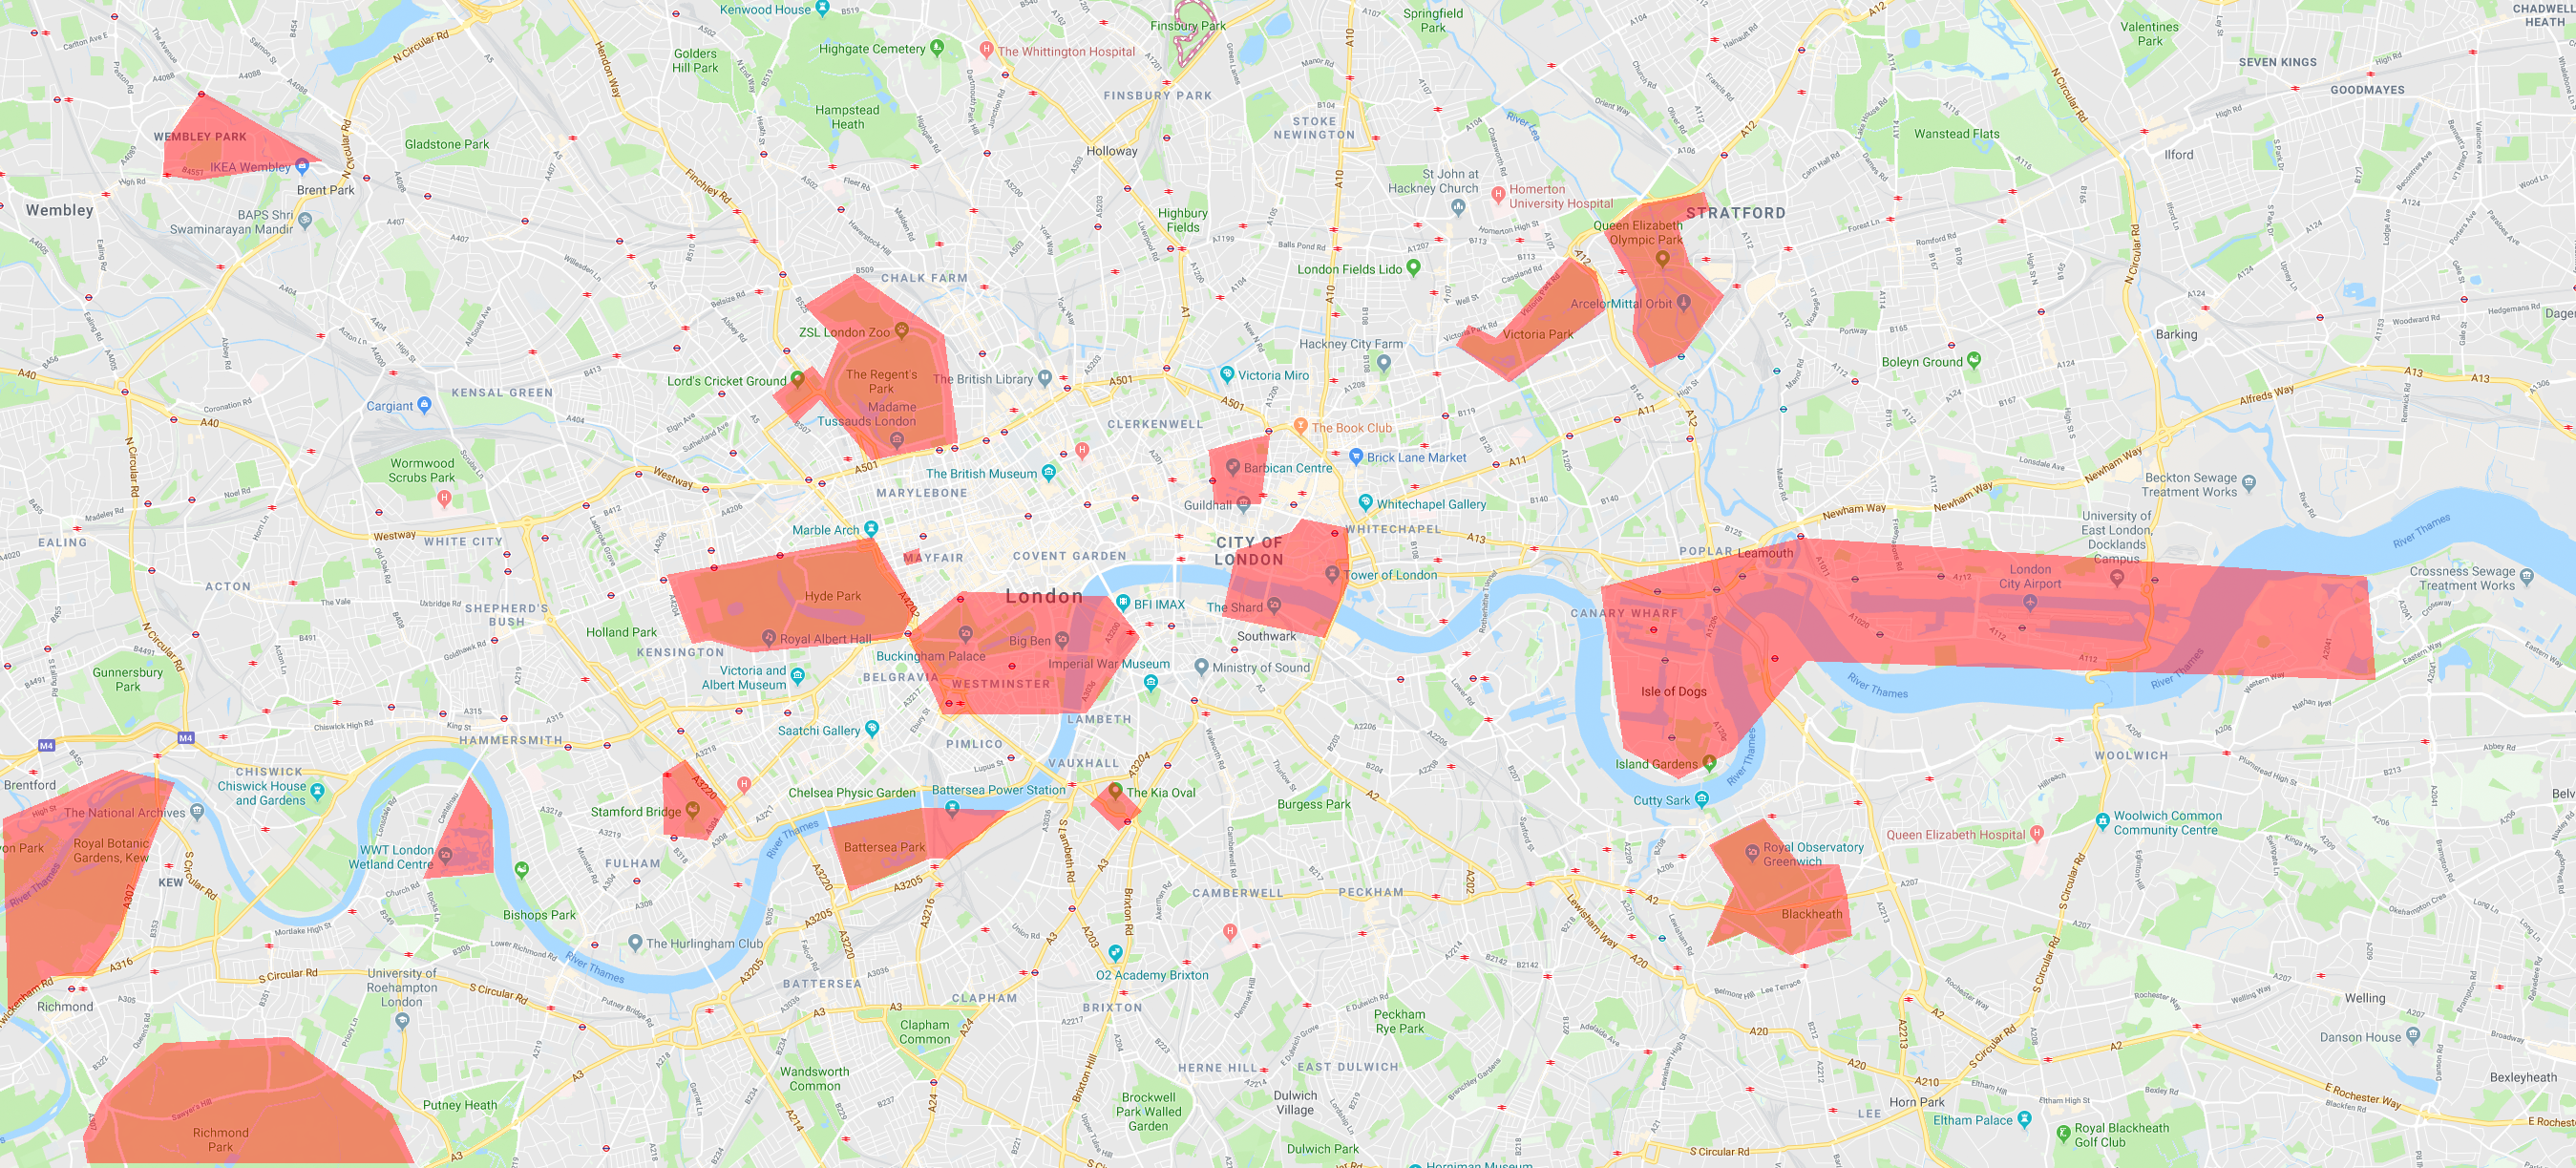
\includegraphics[width=\linewidth]{img/london_snapshot_large_nfzs.png}
  \caption{Our large London snapshot with NFZs highlighted.}
  \label{fig:london_snapshot_large_nfzs}
\end{figure}

We also apply No Fly Zones to cultural and sporting hotspots such as the Oval, Wembley Stadium and the O2. However, we also extend the O2 No Fly Zone across a large stretch of East London in order to cover both the skyscapes of Canary Wharf, and the flight paths of planes coming in and out of London City Airport.

\subsection{Controllers}
Now that we have our world populated with No Fly Zones, we are able to consider how we might choose to configure our Controllers. Placing Controllers near a NFZ reduces their effectiveness because one of the directions around them is not really a feasible option to route drones via.\\

By placing plenty of distance between each Controller and its closest No Fly Zone, we are able to maximise the number of directions that we are able to send drones out to.

\subsubsection{Initial Placement}
\subsubsection{Voronoi Analysis}

\section{Configuring SpatialOS}

\section{Problems}



%**********************************************%
\newpage
\part{Findings}
\chapter{Evaluation}
\section{Metrics}

\subsection{Extracting Log Data}


\section{Comparing Schedulers}
% heavy load vs light load (queue size)
% average profit per Delivery
% total profit
% average rejected potential

\section{Large Scale London Simulation}
% screenshot of Snapshot
% large scale voronoi
% lots of graphs/comparisons
% describe how this system works at scale
% architecture works at scale, still with room for improvement
% Of special interest is the behaviour of the LLV scheduler, as it would only prune items from its queue when a call to return the next \texttt{DeliveryRequest} is made. It remains to be seen whether a Controller running the LLV scheduler will be able to handle the extra CPU and memory burden that this design decision will inflict on it.

%**********************************************%
\newpage
\chapter{Conclusion}

%**********************************************%
\newpage
\chapter{Future Work}
% more scheduling types
% switching scheduler on-the-fly
% introducing more TVFs
% comparing more schedulers
% split-scheduling: half on FCFS, half on priority scheduling?
% order generation to be more representative of real-world package distribution
% drone refuelling
% drones not needing to come back to hub after every delivery
% drones making delivering more than 1 package in a round trip
% drones picking up non-hub packages and delivering to non-hub destinations
% inter-controller communication
% pass request from one hub to another hub if there's spare capacity
% more drone types
% more package types
% UnityClient for interactive simulation
% improved data extraction tool


%**********************************************%
\newpage
\addcontentsline{toc}{section}{References}

\printbibliography

% \newpage
\begin{appendices}
\chapter{Code Listings}
\section{Static No Fly Zone Class}
\begin{sexylisting}[colback=white]{Static No Fly Zone Class}
public static class NoFlyZone
{
    private static bool isInPolygon(
      Improbable.Controller.NoFlyZone nfz,
      Improbable.Vector3f point);

    public static bool hasCollidedWith(
      Improbable.Controller.NoFlyZone nfz,
      Improbable.Vector3f point);

    public static bool hasCollidedWithAny(
      List<Improbable.Controller.NoFlyZone> zones,
      Vector3f point);

    public static void setBoundingBoxCoordinates(
      ref Improbable.Controller.NoFlyZone nfz);

    public static bool isPointInTheBoundingBox(
      Improbable.Controller.NoFlyZone nfz,
      Improbable.Vector3f point);
}
\end{sexylisting}

\section{Nearby Drone and Collision Detection}
\begin{sexylisting}[colback=white]{Nearby Drone and Collision Detection}
private void CheckForNearbyDrones(Vector3 dronePos, bool collisionsOn)
{
  nearestDrone.type = APFObstacleType.NONE;
  nearestDrone.position = new Vector3f(0, -1, 0);
  nearestDroneDistance = radiusOfInfluence;

  Collider[] hitColliders = Physics.OverlapSphere(dronePos, apfRadius);
  foreach (Collider hitCollider in hitColliders)
  {
    if (hitCollider.gameObject.EntityId() != gameObject.EntityId())
    {
      float currentDroneDistance
        = Vector3.Distance(hitCollider.transform.position, dronePos);

      if (collisionsOn && currentDroneDistance < 1)
      {
        /* collision reported to controller */
      }

      if (currentDroneDistance < nearestDroneDistance)
      {
        nearestDrone.position
          = hitCollider.transform.position.ToSpatialVector3f();
        nearestDrone.type = APFObstacleType.DRONE;
        nearestDroneDistance = currentDroneDistance;
      }
    }
  }
}
\end{sexylisting}

\section{Main Controller Loop}
\begin{sexylisting}[colback=white]{Main Controller Loop}
void ControllerTick()
{
  if (!ControllerWriter.Data.initialised)
  {
    /* initialise global layer */
  }

  QueueEntry nextRequest;
  if (ReadyForDeployment())
  {
    if (scheduler.GetNextRequest(out nextRequest))
    {
      HandleDeliveryRequest(nextRequest);
    }
  }

  scheduler.UpdateDeliveryRequestQueue();
}
\end{sexylisting}

\section{Updated DeliveryRequest Generation}
\begin{sexylisting}[colback=white]{Additions to DeliveryHandler Schema}
enum PackageType {
  LETTER_SMALL = 0;
  LETTER_LARGE = 1;
  ENVELOPE_SMALL = 2;
  ENVELOPE_STANDARD = 3;
  ENVELOPE_LARGE = 4;
  PARCEL = 5;
}

type PackageInfo {
  PackageType type = 1;
  float weight = 2;
}

enum DeliveryType {
  STANDARD = 0;
  PRIORITY = 1;
  URGENT = 2;
  SUPER_PRIORITY = 3;
}
\end{sexylisting}

\end{appendices}
\end{document}
